\documentclass[twoside]{book}

% Packages required by doxygen
\usepackage{calc}
\usepackage{doxygen}
\usepackage{graphicx}
\usepackage[utf8]{inputenc}
\usepackage{makeidx}
\usepackage{multicol}
\usepackage{multirow}
\usepackage{textcomp}
\usepackage[table]{xcolor}

% Font selection
\usepackage[T1]{fontenc}
\usepackage{mathptmx}
\usepackage[scaled=.90]{helvet}
\usepackage{courier}
\usepackage{amssymb}
\usepackage{sectsty}
\renewcommand{\familydefault}{\sfdefault}
\allsectionsfont{%
  \fontseries{bc}\selectfont%
  \color{darkgray}%
}
\renewcommand{\DoxyLabelFont}{%
  \fontseries{bc}\selectfont%
  \color{darkgray}%
}

% Page & text layout
\usepackage{geometry}
\geometry{%
  a4paper,%
  top=2.5cm,%
  bottom=2.5cm,%
  left=2.5cm,%
  right=2.5cm%
}
\tolerance=750
\hfuzz=15pt
\hbadness=750
\setlength{\emergencystretch}{15pt}
\setlength{\parindent}{0cm}
\setlength{\parskip}{0.2cm}
\makeatletter
\renewcommand{\paragraph}{%
  \@startsection{paragraph}{4}{0ex}{-1.0ex}{1.0ex}{%
    \normalfont\normalsize\bfseries\SS@parafont%
  }%
}
\renewcommand{\subparagraph}{%
  \@startsection{subparagraph}{5}{0ex}{-1.0ex}{1.0ex}{%
    \normalfont\normalsize\bfseries\SS@subparafont%
  }%
}
\makeatother

% Headers & footers
\usepackage{fancyhdr}
\pagestyle{fancyplain}
\fancyhead[LE]{\fancyplain{}{\bfseries\thepage}}
\fancyhead[CE]{\fancyplain{}{}}
\fancyhead[RE]{\fancyplain{}{\bfseries\leftmark}}
\fancyhead[LO]{\fancyplain{}{\bfseries\rightmark}}
\fancyhead[CO]{\fancyplain{}{}}
\fancyhead[RO]{\fancyplain{}{\bfseries\thepage}}
\fancyfoot[LE]{\fancyplain{}{}}
\fancyfoot[CE]{\fancyplain{}{}}
\fancyfoot[RE]{\fancyplain{}{\bfseries\scriptsize Generated on Wed Apr 8 2015 15\-:12\-:56 for Grog-\/\-Like by Doxygen }}
\fancyfoot[LO]{\fancyplain{}{\bfseries\scriptsize Generated on Wed Apr 8 2015 15\-:12\-:56 for Grog-\/\-Like by Doxygen }}
\fancyfoot[CO]{\fancyplain{}{}}
\fancyfoot[RO]{\fancyplain{}{}}
\renewcommand{\footrulewidth}{0.4pt}
\renewcommand{\chaptermark}[1]{%
  \markboth{#1}{}%
}
\renewcommand{\sectionmark}[1]{%
  \markright{\thesection\ #1}%
}

% Indices & bibliography
\usepackage{natbib}
\usepackage[titles]{tocloft}
\setcounter{tocdepth}{3}
\setcounter{secnumdepth}{5}
\makeindex

% Hyperlinks (required, but should be loaded last)
\usepackage{ifpdf}
\ifpdf
  \usepackage[pdftex,pagebackref=true]{hyperref}
\else
  \usepackage[ps2pdf,pagebackref=true]{hyperref}
\fi
\hypersetup{%
  colorlinks=true,%
  linkcolor=blue,%
  citecolor=blue,%
  unicode%
}

% Custom commands
\newcommand{\clearemptydoublepage}{%
  \newpage{\pagestyle{empty}\cleardoublepage}%
}


%===== C O N T E N T S =====

\begin{document}

% Titlepage & ToC
\hypersetup{pageanchor=false}
\pagenumbering{roman}
\begin{titlepage}
\vspace*{7cm}
\begin{center}%
{\Large Grog-\/\-Like }\\
\vspace*{1cm}
{\large Generated by Doxygen 1.8.5}\\
\vspace*{0.5cm}
{\small Wed Apr 8 2015 15:12:56}\\
\end{center}
\end{titlepage}
\clearemptydoublepage
\tableofcontents
\clearemptydoublepage
\pagenumbering{arabic}
\hypersetup{pageanchor=true}

%--- Begin generated contents ---
\chapter{Todo List}
\label{todo}
\hypertarget{todo}{}

\begin{DoxyRefList}
\item[\label{todo__todo000001}%
\hypertarget{todo__todo000001}{}%
Member \hyperlink{class_characters_aee824830a67177342ae606f959fb0c7a}{Characters\-:\-:\-\_\-pickup\-Item} (int status)]Making throw the old item.  
\item[\label{todo__todo000003}%
\hypertarget{todo__todo000003}{}%
Member \hyperlink{class_consumable_adb866e69c3796edffad832b88e527518}{Consumable\-:\-:Begin\-Contact} (\hyperlink{class_elements}{Elements} $\ast$elem, b2\-Contact $\ast$contact)]\-: This function is actually doing nothing.  
\item[\label{todo__todo000002}%
\hypertarget{todo__todo000002}{}%
Member \hyperlink{class_consumable_ae374944f6333618dd08318b98b6950c7}{Consumable\-:\-:Consumable} ()]\-: This function setting attributes the hard-\/way. Maybe a name based config, like \hyperlink{class_characters}{Characters}, would be better ?  
\item[\label{todo__todo000004}%
\hypertarget{todo__todo000004}{}%
Member \hyperlink{class_equipment_a2bd67c4254f2074f4f7469f29a20e760}{Equipment\-:\-:Equipment} ()]\-: The position is actually in the hard-\/way. Config file needed.  
\item[\label{todo__todo000005}%
\hypertarget{todo__todo000005}{}%
Member \hyperlink{class_game_a194dbc017575c98bda4e2317d266a67e}{Game\-:\-:display\-H\-U\-D} (void)]This function is nasty, we need a recap here.  
\item[\label{todo__todo000007}%
\hypertarget{todo__todo000007}{}%
Member \hyperlink{class_h_u_d_window_a1c6965adb9fdd22b230d20b26fef5ac0}{H\-U\-D\-Window\-:\-:armor} (void)]\-: The description here is a lie. But it's gonna append !  
\item[\label{todo__todo000008}%
\hypertarget{todo__todo000008}{}%
Member \hyperlink{class_h_u_d_window_acd4fdbfd1c2562384b84d3bcda80fea1}{H\-U\-D\-Window\-:\-:boots} (void)]\-: No callback \& object for now, but have to do it !  
\item[\label{todo__todo000009}%
\hypertarget{todo__todo000009}{}%
Member \hyperlink{class_h_u_d_window_a378bc8269cacb151f68cfb37114e0c38}{H\-U\-D\-Window\-:\-:consumable} (void)]\-: Same here, no callback or object.  
\item[\label{todo__todo000006}%
\hypertarget{todo__todo000006}{}%
Member \hyperlink{class_h_u_d_window_a8fc917fbfae792d046e90448c963100a}{H\-U\-D\-Window\-:\-:life} (int l)]\-: Empty heart, half-\/heart.  
\item[\label{todo__todo000010}%
\hypertarget{todo__todo000010}{}%
Member \hyperlink{class_h_u_d_window_a8264836f3c55d8211f4e5166e9049628}{H\-U\-D\-Window\-:\-:minimap} (void)]\-: Make this function work normally. 
\end{DoxyRefList}
\chapter{Hierarchical Index}
\section{Class Hierarchy}
This inheritance list is sorted roughly, but not completely, alphabetically\-:\begin{DoxyCompactList}
\item b2\-Contact\-Filter\begin{DoxyCompactList}
\item \contentsline{section}{Contact\-Filter}{\pageref{class_contact_filter}}{}
\end{DoxyCompactList}
\item b2\-Contact\-Listener\begin{DoxyCompactList}
\item \contentsline{section}{Game\-Contact\-Listener}{\pageref{class_game_contact_listener}}{}
\end{DoxyCompactList}
\item \contentsline{section}{Game}{\pageref{class_game}}{}
\item \contentsline{section}{Hitbox}{\pageref{class_hitbox}}{}
\item H\-U\-D\-Actor\begin{DoxyCompactList}
\item \contentsline{section}{H\-U\-D\-Window}{\pageref{class_h_u_d_window}}{}
\end{DoxyCompactList}
\item \contentsline{section}{Level\-Generator}{\pageref{class_level_generator}}{}
\item \contentsline{section}{Log}{\pageref{class_log}}{}
\item \contentsline{section}{Map}{\pageref{class_map}}{}
\item \contentsline{section}{Maps}{\pageref{class_maps}}{}
\item Mouse\-Listener\begin{DoxyCompactList}
\item \contentsline{section}{Mouse\-Debugger}{\pageref{class_mouse_debugger}}{}
\end{DoxyCompactList}
\item Physics\-Actor\begin{DoxyCompactList}
\item \contentsline{section}{Elements}{\pageref{class_elements}}{}
\begin{DoxyCompactList}
\item \contentsline{section}{Characters}{\pageref{class_characters}}{}
\begin{DoxyCompactList}
\item \contentsline{section}{Enemy}{\pageref{class_enemy}}{}
\item \contentsline{section}{Hero}{\pageref{class_hero}}{}
\end{DoxyCompactList}
\item \contentsline{section}{Object}{\pageref{class_object}}{}
\begin{DoxyCompactList}
\item \contentsline{section}{Consumable}{\pageref{class_consumable}}{}
\item \contentsline{section}{Equipment}{\pageref{class_equipment}}{}
\end{DoxyCompactList}
\item \contentsline{section}{Projectile}{\pageref{class_projectile}}{}
\item \contentsline{section}{Shooter}{\pageref{class_shooter}}{}
\item \contentsline{section}{Weapon}{\pageref{class_weapon}}{}
\item \contentsline{section}{Weapon\-List}{\pageref{class_weapon_list}}{}
\end{DoxyCompactList}
\end{DoxyCompactList}
\item \contentsline{section}{Room}{\pageref{class_room}}{}
\end{DoxyCompactList}

\chapter{Class Index}
\section{Class List}
Here are the classes, structs, unions and interfaces with brief descriptions\-:\begin{DoxyCompactList}
\item\contentsline{section}{\hyperlink{class_characters}{Characters} }{\pageref{class_characters}}{}
\item\contentsline{section}{\hyperlink{class_consumable}{Consumable} }{\pageref{class_consumable}}{}
\item\contentsline{section}{\hyperlink{class_contact_filter}{Contact\-Filter} }{\pageref{class_contact_filter}}{}
\item\contentsline{section}{\hyperlink{class_elements}{Elements} }{\pageref{class_elements}}{}
\item\contentsline{section}{\hyperlink{class_enemy}{Enemy} }{\pageref{class_enemy}}{}
\item\contentsline{section}{\hyperlink{class_equipment}{Equipment} }{\pageref{class_equipment}}{}
\item\contentsline{section}{\hyperlink{class_game}{Game} }{\pageref{class_game}}{}
\item\contentsline{section}{\hyperlink{class_game_contact_listener}{Game\-Contact\-Listener} }{\pageref{class_game_contact_listener}}{}
\item\contentsline{section}{\hyperlink{class_hero}{Hero} }{\pageref{class_hero}}{}
\item\contentsline{section}{\hyperlink{class_hitbox}{Hitbox} }{\pageref{class_hitbox}}{}
\item\contentsline{section}{\hyperlink{class_h_u_d_window}{H\-U\-D\-Window} }{\pageref{class_h_u_d_window}}{}
\item\contentsline{section}{\hyperlink{class_level_generator}{Level\-Generator} }{\pageref{class_level_generator}}{}
\item\contentsline{section}{\hyperlink{class_log}{Log} }{\pageref{class_log}}{}
\item\contentsline{section}{\hyperlink{class_map}{Map} }{\pageref{class_map}}{}
\item\contentsline{section}{\hyperlink{class_maps}{Maps} }{\pageref{class_maps}}{}
\item\contentsline{section}{\hyperlink{class_menu}{Menu} }{\pageref{class_menu}}{}
\item\contentsline{section}{\hyperlink{class_mouse_debugger}{Mouse\-Debugger} }{\pageref{class_mouse_debugger}}{}
\item\contentsline{section}{\hyperlink{class_object}{Object} }{\pageref{class_object}}{}
\item\contentsline{section}{\hyperlink{class_projectile}{Projectile} }{\pageref{class_projectile}}{}
\item\contentsline{section}{\hyperlink{class_room}{Room} }{\pageref{class_room}}{}
\item\contentsline{section}{\hyperlink{class_shooter}{Shooter} }{\pageref{class_shooter}}{}
\item\contentsline{section}{\hyperlink{class_weapon}{Weapon} }{\pageref{class_weapon}}{}
\item\contentsline{section}{\hyperlink{class_weapon_list}{Weapon\-List} }{\pageref{class_weapon_list}}{}
\end{DoxyCompactList}

\chapter{Class Documentation}
\hypertarget{class_characters}{\section{Characters Class Reference}
\label{class_characters}\index{Characters@{Characters}}
}


{\ttfamily \#include $<$Characters.\-hpp$>$}



Inheritance diagram for Characters\-:\nopagebreak
\begin{figure}[H]
\begin{center}
\leavevmode
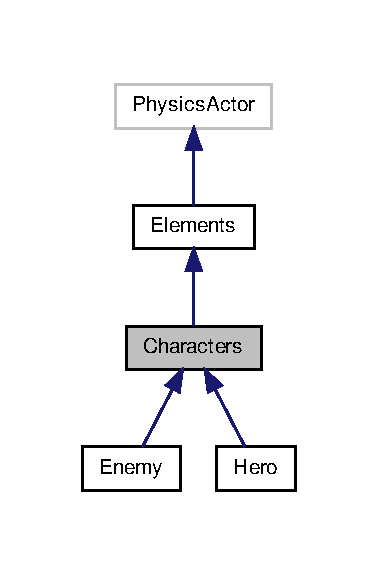
\includegraphics[width=182pt]{class_characters__inherit__graph}
\end{center}
\end{figure}


Collaboration diagram for Characters\-:\nopagebreak
\begin{figure}[H]
\begin{center}
\leavevmode
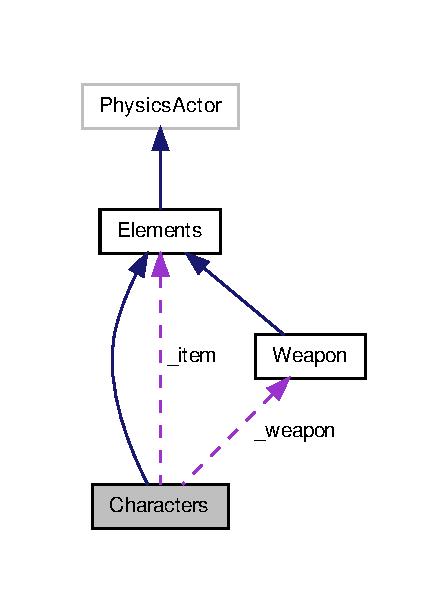
\includegraphics[width=215pt]{class_characters__coll__graph}
\end{center}
\end{figure}
\subsection*{Public Types}
\begin{DoxyCompactItemize}
\item 
enum \hyperlink{class_characters_a95d5115bd36cdc1a7a21ab8c679f7524}{Orientation} \{ \hyperlink{class_characters_a95d5115bd36cdc1a7a21ab8c679f7524ada117a4b1a8823a1056d8bb96a26e607}{U\-P}, 
\hyperlink{class_characters_a95d5115bd36cdc1a7a21ab8c679f7524ae2f08003a915dd35de6b27a8f6c9e992}{D\-O\-W\-N}, 
\hyperlink{class_characters_a95d5115bd36cdc1a7a21ab8c679f7524a553bc25498b5501fb33ae2048c07582d}{L\-E\-F\-T}, 
\hyperlink{class_characters_a95d5115bd36cdc1a7a21ab8c679f7524a58e0c26bba11a4989152f0c3b1bfb4d4}{R\-I\-G\-H\-T}
 \}
\end{DoxyCompactItemize}
\subsection*{Public Member Functions}
\begin{DoxyCompactItemize}
\item 
\hyperlink{class_characters_a3b7d631de563c07caaa918e217a97436}{Characters} (void)
\begin{DoxyCompactList}\small\item\em Base constructor. \end{DoxyCompactList}\item 
\hyperlink{class_characters_a3ebbe5ca8cc3965b55283af002ce8707}{Characters} (std\-::string name)
\begin{DoxyCompactList}\small\item\em Main constructor. \end{DoxyCompactList}\item 
\hyperlink{class_characters_a4aea85daea3f08b8b933e82cd42b3109}{$\sim$\-Characters} ()
\begin{DoxyCompactList}\small\item\em Basic destructor. \end{DoxyCompactList}\item 
virtual void \hyperlink{class_characters_ae6b55c4269efc485d7926f62544eef4e}{Receive\-Message} (Message $\ast$m)
\begin{DoxyCompactList}\small\item\em The Broadcast function of \hyperlink{class_characters}{Characters}. \end{DoxyCompactList}\item 
virtual void \hyperlink{class_characters_a6354b7fd409cde57312c5eca1cf43275}{Anim\-Callback} (String s)
\begin{DoxyCompactList}\small\item\em Animation callback. \end{DoxyCompactList}\item 
virtual void \hyperlink{class_characters_ae1b52f35e60cd23ec118595a9a8e8760}{Begin\-Contact} (\hyperlink{class_elements}{Elements} $\ast$elem, b2\-Contact $\ast$contact)
\begin{DoxyCompactList}\small\item\em Collision function. \end{DoxyCompactList}\item 
virtual void \hyperlink{class_characters_a87c76bb34f5c11e2da4537be07d2f846}{End\-Contact} (\hyperlink{class_elements}{Elements} $\ast$elem, b2\-Contact $\ast$contact)
\begin{DoxyCompactList}\small\item\em End collision function. \end{DoxyCompactList}\item 
\hyperlink{class_characters_a95d5115bd36cdc1a7a21ab8c679f7524}{Characters\-::\-Orientation} \hyperlink{class_characters_a9be6daa0dc468da9c4c0ffa0d0d36ae1}{get\-Orientation} (void)
\item 
std\-::string \hyperlink{class_characters_a0df57bdee9ddc5e4e18954b8b30b1331}{get\-Last\-Action} (void)
\item 
int \hyperlink{class_characters_a136d6ba8b4bd401fda19b14b089a107f}{get\-H\-P} (void)
\item 
void \hyperlink{class_characters_a63874c1b86156aa6c4c6a7c26afef6e7}{set\-H\-P} (int h)
\begin{DoxyCompactList}\small\item\em Set basics hp. \end{DoxyCompactList}\item 
\hyperlink{class_weapon}{Weapon} $\ast$ \hyperlink{class_characters_aae885a7d773657cdf18f8dfced51d1a8}{get\-Weapon} (void)
\item 
virtual void \hyperlink{class_characters_a76e565eca6d40dc04119697e1218d24d}{action\-Callback} (std\-::string name, int status)
\item 
virtual void \hyperlink{class_characters_a99ea3219f0784f29306bfe539301b83a}{equip\-Weapon} (\hyperlink{class_weapon}{Weapon} $\ast$weapon)
\begin{DoxyCompactList}\small\item\em Equip a weapon. \end{DoxyCompactList}\item 
void \hyperlink{class_characters_a542fa5bfc689011ccc0c4cc4edc9d32a}{change\-Can\-Move} (void)
\end{DoxyCompactItemize}
\subsection*{Protected Member Functions}
\begin{DoxyCompactItemize}
\item 
Json\-::\-Value \hyperlink{class_characters_ace37d9664457f555a0009eb5f3b8b6b2}{\-\_\-get\-Attr} (std\-::string category, std\-::string key)
\begin{DoxyCompactList}\small\item\em Get an attribute load in the conf file. \end{DoxyCompactList}\item 
Json\-::\-Value \hyperlink{class_characters_abd51b12301a105d11021ac3302c742ea}{\-\_\-get\-Attr} (std\-::string key)
\begin{DoxyCompactList}\small\item\em Get an attribute with a pre-\/set category. \end{DoxyCompactList}\item 
void \hyperlink{class_characters_a9a06365f3881336e2ee8509129ec54cd}{\-\_\-set\-Category} (std\-::string category)
\begin{DoxyCompactList}\small\item\em Set the current working category. \end{DoxyCompactList}\item 
virtual void \hyperlink{class_characters_af8dca1980a447965ffeb2ea17a507c5c}{\-\_\-forward} (int status)
\begin{DoxyCompactList}\small\item\em Forward action. \end{DoxyCompactList}\item 
virtual void \hyperlink{class_characters_ab5b3e9e9140665e9e358343d9b47ea1c}{\-\_\-backward} (int status)
\begin{DoxyCompactList}\small\item\em Backward action. \end{DoxyCompactList}\item 
virtual void \hyperlink{class_characters_a2bb63a2db8990e516cc2424f1dbf713a}{\-\_\-up} (int status)
\begin{DoxyCompactList}\small\item\em Up button action. \end{DoxyCompactList}\item 
virtual void \hyperlink{class_characters_a3253373f4bf97f623de6d758b464b553}{\-\_\-down} (int status)
\begin{DoxyCompactList}\small\item\em Down button action. \end{DoxyCompactList}\item 
virtual void \hyperlink{class_characters_afad45a33b0277605c50b90031371e00a}{\-\_\-jump} (int status)
\begin{DoxyCompactList}\small\item\em Jump action. \end{DoxyCompactList}\item 
virtual void \hyperlink{class_characters_a9ff6c76cd02e53019e15801e9c76a719}{\-\_\-attack} (int status)
\begin{DoxyCompactList}\small\item\em Attack action. \end{DoxyCompactList}\item 
virtual void \hyperlink{class_characters_aee824830a67177342ae606f959fb0c7a}{\-\_\-pickup\-Item} (int status)
\begin{DoxyCompactList}\small\item\em Pick an item. \end{DoxyCompactList}\item 
virtual void \hyperlink{class_characters_aa59e298bef3e58fc7c82deb86e762200}{\-\_\-run} (void)
\begin{DoxyCompactList}\small\item\em Intern callbacks for moving. \end{DoxyCompactList}\item 
void \hyperlink{class_characters_a98666bfdc74679e0ab605a4f6a89ecb2}{\-\_\-destroy\-Enemy} (void)
\begin{DoxyCompactList}\small\item\em Destroy an \hyperlink{class_enemy}{Enemy}. \end{DoxyCompactList}\end{DoxyCompactItemize}
\subsection*{Protected Attributes}
\begin{DoxyCompactItemize}
\item 
std\-::string \hyperlink{class_characters_aa07da1842926f30143e7504fb6cbeb18}{\-\_\-name}
\item 
std\-::string \hyperlink{class_characters_a7fd13ae98277d01b16ad744852d5bd9a}{\-\_\-last\-Action}
\item 
int \hyperlink{class_characters_a1ea81e7d8e2bfb27f9a55b9aa6fbdd2a}{\-\_\-id}
\item 
int \hyperlink{class_characters_aceee7dd6aae36a7eacefcc276f3423c0}{\-\_\-size}
\item 
int \hyperlink{class_characters_a71736ea7efb50f0174865607d715c8f1}{\-\_\-max\-Speed}
\item 
int \hyperlink{class_characters_a05cdafb4f63caae675982af22c32fba5}{\-\_\-is\-Jump}
\item 
int \hyperlink{class_characters_a9a8242e24955e5a0c75e69598687c55f}{\-\_\-is\-Running}
\item 
int \hyperlink{class_characters_a19ecafdcd8a707d8b3e0fe3c7069b99e}{\-\_\-is\-Attacking}
\item 
int \hyperlink{class_characters_a08ee77521ac4ceaf02fc663e41251e6d}{\-\_\-hp}
\item 
int \hyperlink{class_characters_abc14e96e35df47aba94dbf23b3dbdba6}{\-\_\-max\-Hp}
\item 
bool \hyperlink{class_characters_a817a390b358c806dd3e5c353a815871c}{\-\_\-can\-Move}
\item 
bool \hyperlink{class_characters_a7488ab360a4a770d46a2578f87f02511}{\-\_\-can\-Jump}
\item 
bool \hyperlink{class_characters_a6a43d519e518708eddef2438dae04a1f}{\-\_\-invincibility}
\item 
\hyperlink{class_weapon}{Weapon} $\ast$ \hyperlink{class_characters_aee5f545db9a5e0ee19af66dc0754b602}{\-\_\-weapon}
\item 
\hyperlink{class_elements}{Elements} $\ast$ \hyperlink{class_characters_a0befc3d5cf681d5cd555929ffde0d25a}{\-\_\-item}
\item 
\hyperlink{class_characters_a95d5115bd36cdc1a7a21ab8c679f7524}{Characters\-::\-Orientation} \hyperlink{class_characters_ad1f8866efe25f7c8997a134f536fe121}{\-\_\-orientation}
\item 
\hyperlink{class_characters_a95d5115bd36cdc1a7a21ab8c679f7524}{Characters\-::\-Orientation} \hyperlink{class_characters_a1d78d9a93ebfad3f058a155505257c91}{\-\_\-lat\-Orientation}
\item 
std\-::list$<$ \hyperlink{class_elements}{Elements} $\ast$ $>$ \hyperlink{class_characters_a35ee6e0ded905f63112a08cd3ad76435}{\-\_\-grounds}
\item 
std\-::list$<$ \hyperlink{class_elements}{Elements} $\ast$ $>$ \hyperlink{class_characters_a7a12ea35974e9b9d5fce08b194c37df0}{\-\_\-walls\-Left}
\item 
std\-::list$<$ \hyperlink{class_elements}{Elements} $\ast$ $>$ \hyperlink{class_characters_af296e78457066933b426e1a1e950a9d4}{\-\_\-walls}
\item 
std\-::list$<$ \hyperlink{class_elements}{Elements} $\ast$ $>$ \hyperlink{class_characters_a60b4de9d954c3de8093bfce23e0e0cec}{\-\_\-walls\-Right}
\end{DoxyCompactItemize}
\subsection*{Friends}
\begin{DoxyCompactItemize}
\item 
class \hyperlink{class_characters_aa2fab026580d6f14280c2ffb8063a314}{Game}
\end{DoxyCompactItemize}


\subsection{Member Enumeration Documentation}
\hypertarget{class_characters_a95d5115bd36cdc1a7a21ab8c679f7524}{\index{Characters@{Characters}!Orientation@{Orientation}}
\index{Orientation@{Orientation}!Characters@{Characters}}
\subsubsection[{Orientation}]{\setlength{\rightskip}{0pt plus 5cm}enum {\bf Characters\-::\-Orientation}}}\label{class_characters_a95d5115bd36cdc1a7a21ab8c679f7524}
\begin{Desc}
\item[Enumerator]\par
\begin{description}
\index{U\-P@{U\-P}!Characters@{Characters}}\index{Characters@{Characters}!U\-P@{U\-P}}\item[{\em 
\hypertarget{class_characters_a95d5115bd36cdc1a7a21ab8c679f7524ada117a4b1a8823a1056d8bb96a26e607}{U\-P}\label{class_characters_a95d5115bd36cdc1a7a21ab8c679f7524ada117a4b1a8823a1056d8bb96a26e607}
}]\index{D\-O\-W\-N@{D\-O\-W\-N}!Characters@{Characters}}\index{Characters@{Characters}!D\-O\-W\-N@{D\-O\-W\-N}}\item[{\em 
\hypertarget{class_characters_a95d5115bd36cdc1a7a21ab8c679f7524ae2f08003a915dd35de6b27a8f6c9e992}{D\-O\-W\-N}\label{class_characters_a95d5115bd36cdc1a7a21ab8c679f7524ae2f08003a915dd35de6b27a8f6c9e992}
}]\index{L\-E\-F\-T@{L\-E\-F\-T}!Characters@{Characters}}\index{Characters@{Characters}!L\-E\-F\-T@{L\-E\-F\-T}}\item[{\em 
\hypertarget{class_characters_a95d5115bd36cdc1a7a21ab8c679f7524a553bc25498b5501fb33ae2048c07582d}{L\-E\-F\-T}\label{class_characters_a95d5115bd36cdc1a7a21ab8c679f7524a553bc25498b5501fb33ae2048c07582d}
}]\index{R\-I\-G\-H\-T@{R\-I\-G\-H\-T}!Characters@{Characters}}\index{Characters@{Characters}!R\-I\-G\-H\-T@{R\-I\-G\-H\-T}}\item[{\em 
\hypertarget{class_characters_a95d5115bd36cdc1a7a21ab8c679f7524a58e0c26bba11a4989152f0c3b1bfb4d4}{R\-I\-G\-H\-T}\label{class_characters_a95d5115bd36cdc1a7a21ab8c679f7524a58e0c26bba11a4989152f0c3b1bfb4d4}
}]\end{description}
\end{Desc}


\subsection{Constructor \& Destructor Documentation}
\hypertarget{class_characters_a3b7d631de563c07caaa918e217a97436}{\index{Characters@{Characters}!Characters@{Characters}}
\index{Characters@{Characters}!Characters@{Characters}}
\subsubsection[{Characters}]{\setlength{\rightskip}{0pt plus 5cm}Characters\-::\-Characters (
\begin{DoxyParamCaption}
\item[{void}]{}
\end{DoxyParamCaption}
)}}\label{class_characters_a3b7d631de563c07caaa918e217a97436}


Base constructor. 

Licensed to the Apache Software Foundation (A\-S\-F) under one or more contributor license agreements. See the N\-O\-T\-I\-C\-E file distributed with this work for additional information regarding copyright ownership. The A\-S\-F licenses this file to you under the Apache License, Version 2.\-0 (the \char`\"{}\-License\char`\"{}); you may not use this file except in compliance with the License. You may obtain a copy of the License at

\href{http://www.apache.org/licenses/LICENSE-2.0}{\tt http\-://www.\-apache.\-org/licenses/\-L\-I\-C\-E\-N\-S\-E-\/2.\-0}

Unless required by applicable law or agreed to in writing, software distributed under the License is distributed on an \char`\"{}\-A\-S I\-S\char`\"{} B\-A\-S\-I\-S, W\-I\-T\-H\-O\-U\-T W\-A\-R\-R\-A\-N\-T\-I\-E\-S O\-R C\-O\-N\-D\-I\-T\-I\-O\-N\-S O\-F A\-N\-Y K\-I\-N\-D, either express or implied. See the License for the specific language governing permissions and limitations under the License. File\-: \hyperlink{_characters_8cpp}{Characters.\-cpp} Creation\-: 2015-\/02-\/27 04\-:44 Louis Solofrizzo \href{mailto:louis@ne02ptzero.me}{\tt louis@ne02ptzero.\-me} \hypertarget{class_characters_a3ebbe5ca8cc3965b55283af002ce8707}{\index{Characters@{Characters}!Characters@{Characters}}
\index{Characters@{Characters}!Characters@{Characters}}
\subsubsection[{Characters}]{\setlength{\rightskip}{0pt plus 5cm}Characters\-::\-Characters (
\begin{DoxyParamCaption}
\item[{std\-::string}]{name}
\end{DoxyParamCaption}
)}}\label{class_characters_a3ebbe5ca8cc3965b55283af002ce8707}


Main constructor. 

Setting base physic, some attributes and some intern variables 
\begin{DoxyParams}{Parameters}
{\em name} & The name of the character (\hyperlink{class_enemy}{Enemy}, \hyperlink{class_hero}{Hero}, etc ...) \\
\hline
\end{DoxyParams}
\hypertarget{class_characters_a4aea85daea3f08b8b933e82cd42b3109}{\index{Characters@{Characters}!$\sim$\-Characters@{$\sim$\-Characters}}
\index{$\sim$\-Characters@{$\sim$\-Characters}!Characters@{Characters}}
\subsubsection[{$\sim$\-Characters}]{\setlength{\rightskip}{0pt plus 5cm}Characters\-::$\sim$\-Characters (
\begin{DoxyParamCaption}
\item[{void}]{}
\end{DoxyParamCaption}
)}}\label{class_characters_a4aea85daea3f08b8b933e82cd42b3109}


Basic destructor. 



\subsection{Member Function Documentation}
\hypertarget{class_characters_a9ff6c76cd02e53019e15801e9c76a719}{\index{Characters@{Characters}!\-\_\-attack@{\-\_\-attack}}
\index{\-\_\-attack@{\-\_\-attack}!Characters@{Characters}}
\subsubsection[{\-\_\-attack}]{\setlength{\rightskip}{0pt plus 5cm}void Characters\-::\-\_\-attack (
\begin{DoxyParamCaption}
\item[{int}]{status}
\end{DoxyParamCaption}
)\hspace{0.3cm}{\ttfamily [protected]}, {\ttfamily [virtual]}}}\label{class_characters_a9ff6c76cd02e53019e15801e9c76a719}


Attack action. 

Attack action Call the weapon attack() function. 
\begin{DoxyParams}{Parameters}
{\em status} & The key status (1 $|$ 0) \\
\hline
\end{DoxyParams}
\begin{DoxySeeAlso}{See Also}
\hyperlink{class_weapon_a90b2b26acbbfc87a14786c8859e4a01d}{Weapon\-::attack} 
\end{DoxySeeAlso}
\hypertarget{class_characters_ab5b3e9e9140665e9e358343d9b47ea1c}{\index{Characters@{Characters}!\-\_\-backward@{\-\_\-backward}}
\index{\-\_\-backward@{\-\_\-backward}!Characters@{Characters}}
\subsubsection[{\-\_\-backward}]{\setlength{\rightskip}{0pt plus 5cm}void Characters\-::\-\_\-backward (
\begin{DoxyParamCaption}
\item[{int}]{status}
\end{DoxyParamCaption}
)\hspace{0.3cm}{\ttfamily [protected]}, {\ttfamily [virtual]}}}\label{class_characters_ab5b3e9e9140665e9e358343d9b47ea1c}


Backward action. 

Make the character go backward Same as forward. 
\begin{DoxyParams}{Parameters}
{\em status} & The status of the key (1 $|$ 0) \\
\hline
\end{DoxyParams}
\begin{DoxySeeAlso}{See Also}
\hyperlink{class_characters_af8dca1980a447965ffeb2ea17a507c5c}{Characters\-::\-\_\-forward} 
\end{DoxySeeAlso}
\hypertarget{class_characters_a98666bfdc74679e0ab605a4f6a89ecb2}{\index{Characters@{Characters}!\-\_\-destroy\-Enemy@{\-\_\-destroy\-Enemy}}
\index{\-\_\-destroy\-Enemy@{\-\_\-destroy\-Enemy}!Characters@{Characters}}
\subsubsection[{\-\_\-destroy\-Enemy}]{\setlength{\rightskip}{0pt plus 5cm}void Characters\-::\-\_\-destroy\-Enemy (
\begin{DoxyParamCaption}
\item[{void}]{}
\end{DoxyParamCaption}
)\hspace{0.3cm}{\ttfamily [protected]}}}\label{class_characters_a98666bfdc74679e0ab605a4f6a89ecb2}


Destroy an \hyperlink{class_enemy}{Enemy}. 

Made the\-Switchboard Unsubscribe from the object, and destroy it. \hypertarget{class_characters_a3253373f4bf97f623de6d758b464b553}{\index{Characters@{Characters}!\-\_\-down@{\-\_\-down}}
\index{\-\_\-down@{\-\_\-down}!Characters@{Characters}}
\subsubsection[{\-\_\-down}]{\setlength{\rightskip}{0pt plus 5cm}void Characters\-::\-\_\-down (
\begin{DoxyParamCaption}
\item[{int}]{status}
\end{DoxyParamCaption}
)\hspace{0.3cm}{\ttfamily [protected]}, {\ttfamily [virtual]}}}\label{class_characters_a3253373f4bf97f623de6d758b464b553}


Down button action. 

Called when pressing the D\-O\-W\-N button Same as \hyperlink{class_characters_a2bb63a2db8990e516cc2424f1dbf713a}{Characters\-::\-\_\-up} 
\begin{DoxyParams}{Parameters}
{\em status} & The key status (1 $|$ 0) \\
\hline
\end{DoxyParams}
\begin{DoxySeeAlso}{See Also}
\hyperlink{class_characters_a2bb63a2db8990e516cc2424f1dbf713a}{Characters\-::\-\_\-up} 
\end{DoxySeeAlso}
\hypertarget{class_characters_af8dca1980a447965ffeb2ea17a507c5c}{\index{Characters@{Characters}!\-\_\-forward@{\-\_\-forward}}
\index{\-\_\-forward@{\-\_\-forward}!Characters@{Characters}}
\subsubsection[{\-\_\-forward}]{\setlength{\rightskip}{0pt plus 5cm}void Characters\-::\-\_\-forward (
\begin{DoxyParamCaption}
\item[{int}]{status}
\end{DoxyParamCaption}
)\hspace{0.3cm}{\ttfamily [protected]}, {\ttfamily [virtual]}}}\label{class_characters_af8dca1980a447965ffeb2ea17a507c5c}


Forward action. 

Making a \hyperlink{class_characters}{Characters} run forward. This function handle the power size for moving, sprite animation, basicly everything. So, if you want to make some modification, use the intern callback (\hyperlink{class_elements_a85bc66fe037551fcfa0b606cf32c4478}{Characters\-::callback}), or override this function in the children. But, please, D\-O N\-O\-T modify this one. 
\begin{DoxyParams}{Parameters}
{\em status} & The status of the key (0 $|$ 1) \\
\hline
\end{DoxyParams}
\hypertarget{class_characters_ace37d9664457f555a0009eb5f3b8b6b2}{\index{Characters@{Characters}!\-\_\-get\-Attr@{\-\_\-get\-Attr}}
\index{\-\_\-get\-Attr@{\-\_\-get\-Attr}!Characters@{Characters}}
\subsubsection[{\-\_\-get\-Attr}]{\setlength{\rightskip}{0pt plus 5cm}Json\-::\-Value Characters\-::\-\_\-get\-Attr (
\begin{DoxyParamCaption}
\item[{std\-::string}]{category, }
\item[{std\-::string}]{key}
\end{DoxyParamCaption}
)\hspace{0.3cm}{\ttfamily [protected]}}}\label{class_characters_ace37d9664457f555a0009eb5f3b8b6b2}


Get an attribute load in the conf file. 

Get a Json\-::\-Value of a key in the config file 
\begin{DoxyParams}{Parameters}
{\em category} & The category of the attribute \\
\hline
{\em } & key The name of the attribute \\
\hline
\end{DoxyParams}
\begin{DoxyReturn}{Returns}
A Json\-::\-Value, See the docs of jsoncpp for the utilisation of Json\-::\-Value 
\end{DoxyReturn}
\hypertarget{class_characters_abd51b12301a105d11021ac3302c742ea}{\index{Characters@{Characters}!\-\_\-get\-Attr@{\-\_\-get\-Attr}}
\index{\-\_\-get\-Attr@{\-\_\-get\-Attr}!Characters@{Characters}}
\subsubsection[{\-\_\-get\-Attr}]{\setlength{\rightskip}{0pt plus 5cm}Json\-::\-Value Characters\-::\-\_\-get\-Attr (
\begin{DoxyParamCaption}
\item[{std\-::string}]{key}
\end{DoxyParamCaption}
)\hspace{0.3cm}{\ttfamily [protected]}}}\label{class_characters_abd51b12301a105d11021ac3302c742ea}


Get an attribute with a pre-\/set category. 

Get a Json\-::\-Value of a key in the config file, with a pre-\/set category See \hyperlink{class_characters_a9a06365f3881336e2ee8509129ec54cd}{Characters\-::\-\_\-set\-Category} for more info. 
\begin{DoxyParams}{Parameters}
{\em } & key The name of the attribute \\
\hline
\end{DoxyParams}
\begin{DoxySeeAlso}{See Also}
\hyperlink{class_characters_a9a06365f3881336e2ee8509129ec54cd}{Characters\-::\-\_\-set\-Category} 
\end{DoxySeeAlso}
\hypertarget{class_characters_afad45a33b0277605c50b90031371e00a}{\index{Characters@{Characters}!\-\_\-jump@{\-\_\-jump}}
\index{\-\_\-jump@{\-\_\-jump}!Characters@{Characters}}
\subsubsection[{\-\_\-jump}]{\setlength{\rightskip}{0pt plus 5cm}void Characters\-::\-\_\-jump (
\begin{DoxyParamCaption}
\item[{int}]{status}
\end{DoxyParamCaption}
)\hspace{0.3cm}{\ttfamily [protected]}, {\ttfamily [virtual]}}}\label{class_characters_afad45a33b0277605c50b90031371e00a}


Jump action. 

Make the character jump. Same as forward. 
\begin{DoxyParams}{Parameters}
{\em } & status The key status (1 $|$ 0) \\
\hline
\end{DoxyParams}
\begin{DoxySeeAlso}{See Also}
\hyperlink{class_characters_af8dca1980a447965ffeb2ea17a507c5c}{Characters\-::\-\_\-forward} 
\end{DoxySeeAlso}
\hypertarget{class_characters_aee824830a67177342ae606f959fb0c7a}{\index{Characters@{Characters}!\-\_\-pickup\-Item@{\-\_\-pickup\-Item}}
\index{\-\_\-pickup\-Item@{\-\_\-pickup\-Item}!Characters@{Characters}}
\subsubsection[{\-\_\-pickup\-Item}]{\setlength{\rightskip}{0pt plus 5cm}void Characters\-::\-\_\-pickup\-Item (
\begin{DoxyParamCaption}
\item[{int}]{status}
\end{DoxyParamCaption}
)\hspace{0.3cm}{\ttfamily [protected]}, {\ttfamily [virtual]}}}\label{class_characters_aee824830a67177342ae606f959fb0c7a}


Pick an item. 

Pick an item on the floor Replace the current relatable item by the new one. \begin{DoxyRefDesc}{Todo}
\item[\hyperlink{todo__todo000001}{Todo}]Making throw the old item. \end{DoxyRefDesc}

\begin{DoxyParams}{Parameters}
{\em status} & The key status (1 $|$ 0) \\
\hline
\end{DoxyParams}
\hypertarget{class_characters_aa59e298bef3e58fc7c82deb86e762200}{\index{Characters@{Characters}!\-\_\-run@{\-\_\-run}}
\index{\-\_\-run@{\-\_\-run}!Characters@{Characters}}
\subsubsection[{\-\_\-run}]{\setlength{\rightskip}{0pt plus 5cm}void Characters\-::\-\_\-run (
\begin{DoxyParamCaption}
\item[{void}]{}
\end{DoxyParamCaption}
)\hspace{0.3cm}{\ttfamily [protected]}, {\ttfamily [virtual]}}}\label{class_characters_aa59e298bef3e58fc7c82deb86e762200}


Intern callbacks for moving. 

Intern callbacks for making a character move. This function handle the direction of the character. This callback is called in \hyperlink{class_game_ae763ecd953645a586b638a46b908ca5a}{Game\-::make\-It\-Run}, so you probalby don't want to call it. \begin{DoxySeeAlso}{See Also}
\hyperlink{class_game_ae763ecd953645a586b638a46b908ca5a}{Game\-::make\-It\-Run} 
\end{DoxySeeAlso}


Reimplemented from \hyperlink{class_elements_aa367c1471a9fc7f1a9b7b124e69c3ef3}{Elements}.

\hypertarget{class_characters_a9a06365f3881336e2ee8509129ec54cd}{\index{Characters@{Characters}!\-\_\-set\-Category@{\-\_\-set\-Category}}
\index{\-\_\-set\-Category@{\-\_\-set\-Category}!Characters@{Characters}}
\subsubsection[{\-\_\-set\-Category}]{\setlength{\rightskip}{0pt plus 5cm}void Characters\-::\-\_\-set\-Category (
\begin{DoxyParamCaption}
\item[{std\-::string}]{category}
\end{DoxyParamCaption}
)\hspace{0.3cm}{\ttfamily [protected]}}}\label{class_characters_a9a06365f3881336e2ee8509129ec54cd}


Set the current working category. 

This function is made for gain time and money, set first the category in this functions then call the function \hyperlink{class_characters_abd51b12301a105d11021ac3302c742ea}{\-\_\-get\-Attr(std\-::string key)}. See \hyperlink{class_characters_abd51b12301a105d11021ac3302c742ea}{\-\_\-get\-Attr(std\-::string key)} for more info. 
\begin{DoxyParams}{Parameters}
{\em category} & The name of the category \\
\hline
\end{DoxyParams}
\begin{DoxySeeAlso}{See Also}
\hyperlink{class_characters_ace37d9664457f555a0009eb5f3b8b6b2}{Characters\-::\-\_\-get\-Attr} 
\end{DoxySeeAlso}
\hypertarget{class_characters_a2bb63a2db8990e516cc2424f1dbf713a}{\index{Characters@{Characters}!\-\_\-up@{\-\_\-up}}
\index{\-\_\-up@{\-\_\-up}!Characters@{Characters}}
\subsubsection[{\-\_\-up}]{\setlength{\rightskip}{0pt plus 5cm}void Characters\-::\-\_\-up (
\begin{DoxyParamCaption}
\item[{int}]{status}
\end{DoxyParamCaption}
)\hspace{0.3cm}{\ttfamily [protected]}, {\ttfamily [virtual]}}}\label{class_characters_a2bb63a2db8990e516cc2424f1dbf713a}


Up button action. 

Called when pressing the U\-P button This function handle just the Orientation. 
\begin{DoxyParams}{Parameters}
{\em status} & The key status (1 $|$ 0) \\
\hline
\end{DoxyParams}
\hypertarget{class_characters_a76e565eca6d40dc04119697e1218d24d}{\index{Characters@{Characters}!action\-Callback@{action\-Callback}}
\index{action\-Callback@{action\-Callback}!Characters@{Characters}}
\subsubsection[{action\-Callback}]{\setlength{\rightskip}{0pt plus 5cm}virtual void Characters\-::action\-Callback (
\begin{DoxyParamCaption}
\item[{std\-::string}]{name, }
\item[{int}]{status}
\end{DoxyParamCaption}
)\hspace{0.3cm}{\ttfamily [inline]}, {\ttfamily [virtual]}}}\label{class_characters_a76e565eca6d40dc04119697e1218d24d}


Reimplemented in \hyperlink{class_hero_aa41ef53abd25057ceb431811ccf80ad5}{Hero}, and \hyperlink{class_enemy_a2f1157b7c8d74371c2b06493563423ee}{Enemy}.

\hypertarget{class_characters_a6354b7fd409cde57312c5eca1cf43275}{\index{Characters@{Characters}!Anim\-Callback@{Anim\-Callback}}
\index{Anim\-Callback@{Anim\-Callback}!Characters@{Characters}}
\subsubsection[{Anim\-Callback}]{\setlength{\rightskip}{0pt plus 5cm}void Characters\-::\-Anim\-Callback (
\begin{DoxyParamCaption}
\item[{String}]{s}
\end{DoxyParamCaption}
)\hspace{0.3cm}{\ttfamily [virtual]}}}\label{class_characters_a6354b7fd409cde57312c5eca1cf43275}


Animation callback. 

The animation callback See Angel doc for more information String is the std\-::string object used in Angel2d. 
\begin{DoxyParams}{Parameters}
{\em s} & The name of the callback \\
\hline
\end{DoxyParams}
\hypertarget{class_characters_ae1b52f35e60cd23ec118595a9a8e8760}{\index{Characters@{Characters}!Begin\-Contact@{Begin\-Contact}}
\index{Begin\-Contact@{Begin\-Contact}!Characters@{Characters}}
\subsubsection[{Begin\-Contact}]{\setlength{\rightskip}{0pt plus 5cm}void Characters\-::\-Begin\-Contact (
\begin{DoxyParamCaption}
\item[{{\bf Elements} $\ast$}]{elem, }
\item[{b2\-Contact $\ast$}]{contact}
\end{DoxyParamCaption}
)\hspace{0.3cm}{\ttfamily [virtual]}}}\label{class_characters_ae1b52f35e60cd23ec118595a9a8e8760}


Collision function. 

Collision begin callback See Angel docs for more information. /!\textbackslash{} This function is called B\-E\-F\-O\-R\-E a collision happened. 
\begin{DoxyParams}{Parameters}
{\em elem} & The Element who collide \\
\hline
{\em contact} & The b2\-Contact object of the collision. See Box2\-D docs for more info. \\
\hline
\end{DoxyParams}


Reimplemented from \hyperlink{class_elements_a108938e08197adc349e98fb91abe1b5a}{Elements}.



Reimplemented in \hyperlink{class_enemy_a3938e3e2cf5f07d809e1f1927b09539a}{Enemy}, and \hyperlink{class_hero_ac23c090d8f5e2768b4175580a0d53d1b}{Hero}.

\hypertarget{class_characters_a542fa5bfc689011ccc0c4cc4edc9d32a}{\index{Characters@{Characters}!change\-Can\-Move@{change\-Can\-Move}}
\index{change\-Can\-Move@{change\-Can\-Move}!Characters@{Characters}}
\subsubsection[{change\-Can\-Move}]{\setlength{\rightskip}{0pt plus 5cm}void Characters\-::change\-Can\-Move (
\begin{DoxyParamCaption}
\item[{void}]{}
\end{DoxyParamCaption}
)}}\label{class_characters_a542fa5bfc689011ccc0c4cc4edc9d32a}
\hypertarget{class_characters_a87c76bb34f5c11e2da4537be07d2f846}{\index{Characters@{Characters}!End\-Contact@{End\-Contact}}
\index{End\-Contact@{End\-Contact}!Characters@{Characters}}
\subsubsection[{End\-Contact}]{\setlength{\rightskip}{0pt plus 5cm}void Characters\-::\-End\-Contact (
\begin{DoxyParamCaption}
\item[{{\bf Elements} $\ast$}]{elem, }
\item[{b2\-Contact $\ast$}]{contact}
\end{DoxyParamCaption}
)\hspace{0.3cm}{\ttfamily [virtual]}}}\label{class_characters_a87c76bb34f5c11e2da4537be07d2f846}


End collision function. 

Collision end callback /!\textbackslash{} This function is called A\-F\-T\-E\-R the elements leave another 
\begin{DoxyParams}{Parameters}
{\em elem} & The Element who left collision \\
\hline
{\em } & contact The b2\-Contact object of the collided element. See Box2\-D docs for more info. \\
\hline
\end{DoxyParams}


Reimplemented from \hyperlink{class_elements_a42c3b694edefcc789109bd952a66d918}{Elements}.



Reimplemented in \hyperlink{class_hero_a9fee92d1b0df478f95bc10ba84015d2a}{Hero}.

\hypertarget{class_characters_a99ea3219f0784f29306bfe539301b83a}{\index{Characters@{Characters}!equip\-Weapon@{equip\-Weapon}}
\index{equip\-Weapon@{equip\-Weapon}!Characters@{Characters}}
\subsubsection[{equip\-Weapon}]{\setlength{\rightskip}{0pt plus 5cm}void Characters\-::equip\-Weapon (
\begin{DoxyParamCaption}
\item[{{\bf Weapon} $\ast$}]{weapon}
\end{DoxyParamCaption}
)\hspace{0.3cm}{\ttfamily [virtual]}}}\label{class_characters_a99ea3219f0784f29306bfe539301b83a}


Equip a weapon. 

Equip a new weapon to the Character, and update the H\-U\-D.  The \hyperlink{class_weapon}{Weapon} object \hypertarget{class_characters_a136d6ba8b4bd401fda19b14b089a107f}{\index{Characters@{Characters}!get\-H\-P@{get\-H\-P}}
\index{get\-H\-P@{get\-H\-P}!Characters@{Characters}}
\subsubsection[{get\-H\-P}]{\setlength{\rightskip}{0pt plus 5cm}int Characters\-::get\-H\-P (
\begin{DoxyParamCaption}
\item[{void}]{}
\end{DoxyParamCaption}
)}}\label{class_characters_a136d6ba8b4bd401fda19b14b089a107f}
\hypertarget{class_characters_a0df57bdee9ddc5e4e18954b8b30b1331}{\index{Characters@{Characters}!get\-Last\-Action@{get\-Last\-Action}}
\index{get\-Last\-Action@{get\-Last\-Action}!Characters@{Characters}}
\subsubsection[{get\-Last\-Action}]{\setlength{\rightskip}{0pt plus 5cm}std\-::string Characters\-::get\-Last\-Action (
\begin{DoxyParamCaption}
\item[{void}]{}
\end{DoxyParamCaption}
)}}\label{class_characters_a0df57bdee9ddc5e4e18954b8b30b1331}
\hypertarget{class_characters_a9be6daa0dc468da9c4c0ffa0d0d36ae1}{\index{Characters@{Characters}!get\-Orientation@{get\-Orientation}}
\index{get\-Orientation@{get\-Orientation}!Characters@{Characters}}
\subsubsection[{get\-Orientation}]{\setlength{\rightskip}{0pt plus 5cm}{\bf Characters\-::\-Orientation} Characters\-::get\-Orientation (
\begin{DoxyParamCaption}
\item[{void}]{}
\end{DoxyParamCaption}
)}}\label{class_characters_a9be6daa0dc468da9c4c0ffa0d0d36ae1}
\hypertarget{class_characters_aae885a7d773657cdf18f8dfced51d1a8}{\index{Characters@{Characters}!get\-Weapon@{get\-Weapon}}
\index{get\-Weapon@{get\-Weapon}!Characters@{Characters}}
\subsubsection[{get\-Weapon}]{\setlength{\rightskip}{0pt plus 5cm}{\bf Weapon} $\ast$ Characters\-::get\-Weapon (
\begin{DoxyParamCaption}
\item[{void}]{}
\end{DoxyParamCaption}
)}}\label{class_characters_aae885a7d773657cdf18f8dfced51d1a8}
\hypertarget{class_characters_ae6b55c4269efc485d7926f62544eef4e}{\index{Characters@{Characters}!Receive\-Message@{Receive\-Message}}
\index{Receive\-Message@{Receive\-Message}!Characters@{Characters}}
\subsubsection[{Receive\-Message}]{\setlength{\rightskip}{0pt plus 5cm}void Characters\-::\-Receive\-Message (
\begin{DoxyParamCaption}
\item[{Message $\ast$}]{m}
\end{DoxyParamCaption}
)\hspace{0.3cm}{\ttfamily [virtual]}}}\label{class_characters_ae6b55c4269efc485d7926f62544eef4e}


The Broadcast function of \hyperlink{class_characters}{Characters}. 

Receive and redistribute broadcasts messages In this function, we call also the callback function of the child. For more info on this, go to \hyperlink{class_elements_a85bc66fe037551fcfa0b606cf32c4478}{Characters\-::callback} 
\begin{DoxyParams}{Parameters}
{\em } & m The Message object \\
\hline
\end{DoxyParams}
\begin{DoxySeeAlso}{See Also}
\hyperlink{class_elements_a85bc66fe037551fcfa0b606cf32c4478}{Characters\-::callback} 
\end{DoxySeeAlso}
\hypertarget{class_characters_a63874c1b86156aa6c4c6a7c26afef6e7}{\index{Characters@{Characters}!set\-H\-P@{set\-H\-P}}
\index{set\-H\-P@{set\-H\-P}!Characters@{Characters}}
\subsubsection[{set\-H\-P}]{\setlength{\rightskip}{0pt plus 5cm}void Characters\-::set\-H\-P (
\begin{DoxyParamCaption}
\item[{int}]{hp}
\end{DoxyParamCaption}
)}}\label{class_characters_a63874c1b86156aa6c4c6a7c26afef6e7}


Set basics hp. 

Set H\-P to the Character. 
\begin{DoxyParams}{Parameters}
{\em hp} & The H\-P number \\
\hline
\end{DoxyParams}


\subsection{Friends And Related Function Documentation}
\hypertarget{class_characters_aa2fab026580d6f14280c2ffb8063a314}{\index{Characters@{Characters}!Game@{Game}}
\index{Game@{Game}!Characters@{Characters}}
\subsubsection[{Game}]{\setlength{\rightskip}{0pt plus 5cm}friend class {\bf Game}\hspace{0.3cm}{\ttfamily [friend]}}}\label{class_characters_aa2fab026580d6f14280c2ffb8063a314}


\subsection{Member Data Documentation}
\hypertarget{class_characters_a7488ab360a4a770d46a2578f87f02511}{\index{Characters@{Characters}!\-\_\-can\-Jump@{\-\_\-can\-Jump}}
\index{\-\_\-can\-Jump@{\-\_\-can\-Jump}!Characters@{Characters}}
\subsubsection[{\-\_\-can\-Jump}]{\setlength{\rightskip}{0pt plus 5cm}bool Characters\-::\-\_\-can\-Jump\hspace{0.3cm}{\ttfamily [protected]}}}\label{class_characters_a7488ab360a4a770d46a2578f87f02511}
\hypertarget{class_characters_a817a390b358c806dd3e5c353a815871c}{\index{Characters@{Characters}!\-\_\-can\-Move@{\-\_\-can\-Move}}
\index{\-\_\-can\-Move@{\-\_\-can\-Move}!Characters@{Characters}}
\subsubsection[{\-\_\-can\-Move}]{\setlength{\rightskip}{0pt plus 5cm}bool Characters\-::\-\_\-can\-Move\hspace{0.3cm}{\ttfamily [protected]}}}\label{class_characters_a817a390b358c806dd3e5c353a815871c}
\hypertarget{class_characters_a35ee6e0ded905f63112a08cd3ad76435}{\index{Characters@{Characters}!\-\_\-grounds@{\-\_\-grounds}}
\index{\-\_\-grounds@{\-\_\-grounds}!Characters@{Characters}}
\subsubsection[{\-\_\-grounds}]{\setlength{\rightskip}{0pt plus 5cm}std\-::list$<${\bf Elements}$\ast$$>$ Characters\-::\-\_\-grounds\hspace{0.3cm}{\ttfamily [protected]}}}\label{class_characters_a35ee6e0ded905f63112a08cd3ad76435}
\hypertarget{class_characters_a08ee77521ac4ceaf02fc663e41251e6d}{\index{Characters@{Characters}!\-\_\-hp@{\-\_\-hp}}
\index{\-\_\-hp@{\-\_\-hp}!Characters@{Characters}}
\subsubsection[{\-\_\-hp}]{\setlength{\rightskip}{0pt plus 5cm}int Characters\-::\-\_\-hp\hspace{0.3cm}{\ttfamily [protected]}}}\label{class_characters_a08ee77521ac4ceaf02fc663e41251e6d}
\hypertarget{class_characters_a1ea81e7d8e2bfb27f9a55b9aa6fbdd2a}{\index{Characters@{Characters}!\-\_\-id@{\-\_\-id}}
\index{\-\_\-id@{\-\_\-id}!Characters@{Characters}}
\subsubsection[{\-\_\-id}]{\setlength{\rightskip}{0pt plus 5cm}int Characters\-::\-\_\-id\hspace{0.3cm}{\ttfamily [protected]}}}\label{class_characters_a1ea81e7d8e2bfb27f9a55b9aa6fbdd2a}
\hypertarget{class_characters_a6a43d519e518708eddef2438dae04a1f}{\index{Characters@{Characters}!\-\_\-invincibility@{\-\_\-invincibility}}
\index{\-\_\-invincibility@{\-\_\-invincibility}!Characters@{Characters}}
\subsubsection[{\-\_\-invincibility}]{\setlength{\rightskip}{0pt plus 5cm}bool Characters\-::\-\_\-invincibility\hspace{0.3cm}{\ttfamily [protected]}}}\label{class_characters_a6a43d519e518708eddef2438dae04a1f}
\hypertarget{class_characters_a19ecafdcd8a707d8b3e0fe3c7069b99e}{\index{Characters@{Characters}!\-\_\-is\-Attacking@{\-\_\-is\-Attacking}}
\index{\-\_\-is\-Attacking@{\-\_\-is\-Attacking}!Characters@{Characters}}
\subsubsection[{\-\_\-is\-Attacking}]{\setlength{\rightskip}{0pt plus 5cm}int Characters\-::\-\_\-is\-Attacking\hspace{0.3cm}{\ttfamily [protected]}}}\label{class_characters_a19ecafdcd8a707d8b3e0fe3c7069b99e}
\hypertarget{class_characters_a05cdafb4f63caae675982af22c32fba5}{\index{Characters@{Characters}!\-\_\-is\-Jump@{\-\_\-is\-Jump}}
\index{\-\_\-is\-Jump@{\-\_\-is\-Jump}!Characters@{Characters}}
\subsubsection[{\-\_\-is\-Jump}]{\setlength{\rightskip}{0pt plus 5cm}int Characters\-::\-\_\-is\-Jump\hspace{0.3cm}{\ttfamily [protected]}}}\label{class_characters_a05cdafb4f63caae675982af22c32fba5}
\hypertarget{class_characters_a9a8242e24955e5a0c75e69598687c55f}{\index{Characters@{Characters}!\-\_\-is\-Running@{\-\_\-is\-Running}}
\index{\-\_\-is\-Running@{\-\_\-is\-Running}!Characters@{Characters}}
\subsubsection[{\-\_\-is\-Running}]{\setlength{\rightskip}{0pt plus 5cm}int Characters\-::\-\_\-is\-Running\hspace{0.3cm}{\ttfamily [protected]}}}\label{class_characters_a9a8242e24955e5a0c75e69598687c55f}
\hypertarget{class_characters_a0befc3d5cf681d5cd555929ffde0d25a}{\index{Characters@{Characters}!\-\_\-item@{\-\_\-item}}
\index{\-\_\-item@{\-\_\-item}!Characters@{Characters}}
\subsubsection[{\-\_\-item}]{\setlength{\rightskip}{0pt plus 5cm}{\bf Elements}$\ast$ Characters\-::\-\_\-item\hspace{0.3cm}{\ttfamily [protected]}}}\label{class_characters_a0befc3d5cf681d5cd555929ffde0d25a}
\hypertarget{class_characters_a7fd13ae98277d01b16ad744852d5bd9a}{\index{Characters@{Characters}!\-\_\-last\-Action@{\-\_\-last\-Action}}
\index{\-\_\-last\-Action@{\-\_\-last\-Action}!Characters@{Characters}}
\subsubsection[{\-\_\-last\-Action}]{\setlength{\rightskip}{0pt plus 5cm}std\-::string Characters\-::\-\_\-last\-Action\hspace{0.3cm}{\ttfamily [protected]}}}\label{class_characters_a7fd13ae98277d01b16ad744852d5bd9a}
\hypertarget{class_characters_a1d78d9a93ebfad3f058a155505257c91}{\index{Characters@{Characters}!\-\_\-lat\-Orientation@{\-\_\-lat\-Orientation}}
\index{\-\_\-lat\-Orientation@{\-\_\-lat\-Orientation}!Characters@{Characters}}
\subsubsection[{\-\_\-lat\-Orientation}]{\setlength{\rightskip}{0pt plus 5cm}{\bf Characters\-::\-Orientation} Characters\-::\-\_\-lat\-Orientation\hspace{0.3cm}{\ttfamily [protected]}}}\label{class_characters_a1d78d9a93ebfad3f058a155505257c91}
\hypertarget{class_characters_abc14e96e35df47aba94dbf23b3dbdba6}{\index{Characters@{Characters}!\-\_\-max\-Hp@{\-\_\-max\-Hp}}
\index{\-\_\-max\-Hp@{\-\_\-max\-Hp}!Characters@{Characters}}
\subsubsection[{\-\_\-max\-Hp}]{\setlength{\rightskip}{0pt plus 5cm}int Characters\-::\-\_\-max\-Hp\hspace{0.3cm}{\ttfamily [protected]}}}\label{class_characters_abc14e96e35df47aba94dbf23b3dbdba6}
\hypertarget{class_characters_a71736ea7efb50f0174865607d715c8f1}{\index{Characters@{Characters}!\-\_\-max\-Speed@{\-\_\-max\-Speed}}
\index{\-\_\-max\-Speed@{\-\_\-max\-Speed}!Characters@{Characters}}
\subsubsection[{\-\_\-max\-Speed}]{\setlength{\rightskip}{0pt plus 5cm}int Characters\-::\-\_\-max\-Speed\hspace{0.3cm}{\ttfamily [protected]}}}\label{class_characters_a71736ea7efb50f0174865607d715c8f1}
\hypertarget{class_characters_aa07da1842926f30143e7504fb6cbeb18}{\index{Characters@{Characters}!\-\_\-name@{\-\_\-name}}
\index{\-\_\-name@{\-\_\-name}!Characters@{Characters}}
\subsubsection[{\-\_\-name}]{\setlength{\rightskip}{0pt plus 5cm}std\-::string Characters\-::\-\_\-name\hspace{0.3cm}{\ttfamily [protected]}}}\label{class_characters_aa07da1842926f30143e7504fb6cbeb18}
\hypertarget{class_characters_ad1f8866efe25f7c8997a134f536fe121}{\index{Characters@{Characters}!\-\_\-orientation@{\-\_\-orientation}}
\index{\-\_\-orientation@{\-\_\-orientation}!Characters@{Characters}}
\subsubsection[{\-\_\-orientation}]{\setlength{\rightskip}{0pt plus 5cm}{\bf Characters\-::\-Orientation} Characters\-::\-\_\-orientation\hspace{0.3cm}{\ttfamily [protected]}}}\label{class_characters_ad1f8866efe25f7c8997a134f536fe121}
\hypertarget{class_characters_aceee7dd6aae36a7eacefcc276f3423c0}{\index{Characters@{Characters}!\-\_\-size@{\-\_\-size}}
\index{\-\_\-size@{\-\_\-size}!Characters@{Characters}}
\subsubsection[{\-\_\-size}]{\setlength{\rightskip}{0pt plus 5cm}int Characters\-::\-\_\-size\hspace{0.3cm}{\ttfamily [protected]}}}\label{class_characters_aceee7dd6aae36a7eacefcc276f3423c0}
\hypertarget{class_characters_af296e78457066933b426e1a1e950a9d4}{\index{Characters@{Characters}!\-\_\-walls@{\-\_\-walls}}
\index{\-\_\-walls@{\-\_\-walls}!Characters@{Characters}}
\subsubsection[{\-\_\-walls}]{\setlength{\rightskip}{0pt plus 5cm}std\-::list$<${\bf Elements}$\ast$$>$ Characters\-::\-\_\-walls\hspace{0.3cm}{\ttfamily [protected]}}}\label{class_characters_af296e78457066933b426e1a1e950a9d4}
\hypertarget{class_characters_a7a12ea35974e9b9d5fce08b194c37df0}{\index{Characters@{Characters}!\-\_\-walls\-Left@{\-\_\-walls\-Left}}
\index{\-\_\-walls\-Left@{\-\_\-walls\-Left}!Characters@{Characters}}
\subsubsection[{\-\_\-walls\-Left}]{\setlength{\rightskip}{0pt plus 5cm}std\-::list$<${\bf Elements}$\ast$$>$ Characters\-::\-\_\-walls\-Left\hspace{0.3cm}{\ttfamily [protected]}}}\label{class_characters_a7a12ea35974e9b9d5fce08b194c37df0}
\hypertarget{class_characters_a60b4de9d954c3de8093bfce23e0e0cec}{\index{Characters@{Characters}!\-\_\-walls\-Right@{\-\_\-walls\-Right}}
\index{\-\_\-walls\-Right@{\-\_\-walls\-Right}!Characters@{Characters}}
\subsubsection[{\-\_\-walls\-Right}]{\setlength{\rightskip}{0pt plus 5cm}std\-::list$<${\bf Elements}$\ast$$>$ Characters\-::\-\_\-walls\-Right\hspace{0.3cm}{\ttfamily [protected]}}}\label{class_characters_a60b4de9d954c3de8093bfce23e0e0cec}
\hypertarget{class_characters_aee5f545db9a5e0ee19af66dc0754b602}{\index{Characters@{Characters}!\-\_\-weapon@{\-\_\-weapon}}
\index{\-\_\-weapon@{\-\_\-weapon}!Characters@{Characters}}
\subsubsection[{\-\_\-weapon}]{\setlength{\rightskip}{0pt plus 5cm}{\bf Weapon}$\ast$ Characters\-::\-\_\-weapon\hspace{0.3cm}{\ttfamily [protected]}}}\label{class_characters_aee5f545db9a5e0ee19af66dc0754b602}


The documentation for this class was generated from the following files\-:\begin{DoxyCompactItemize}
\item 
/home/louis/\-Documents/rogue-\/like/\-Sources/inc/\hyperlink{_characters_8hpp}{Characters.\-hpp}\item 
/home/louis/\-Documents/rogue-\/like/\-Sources/src/\hyperlink{_characters_8cpp}{Characters.\-cpp}\end{DoxyCompactItemize}

\hypertarget{class_consumable}{\section{Consumable Class Reference}
\label{class_consumable}\index{Consumable@{Consumable}}
}


{\ttfamily \#include $<$Consumable.\+hpp$>$}

Inheritance diagram for Consumable\+:\begin{figure}[H]
\begin{center}
\leavevmode
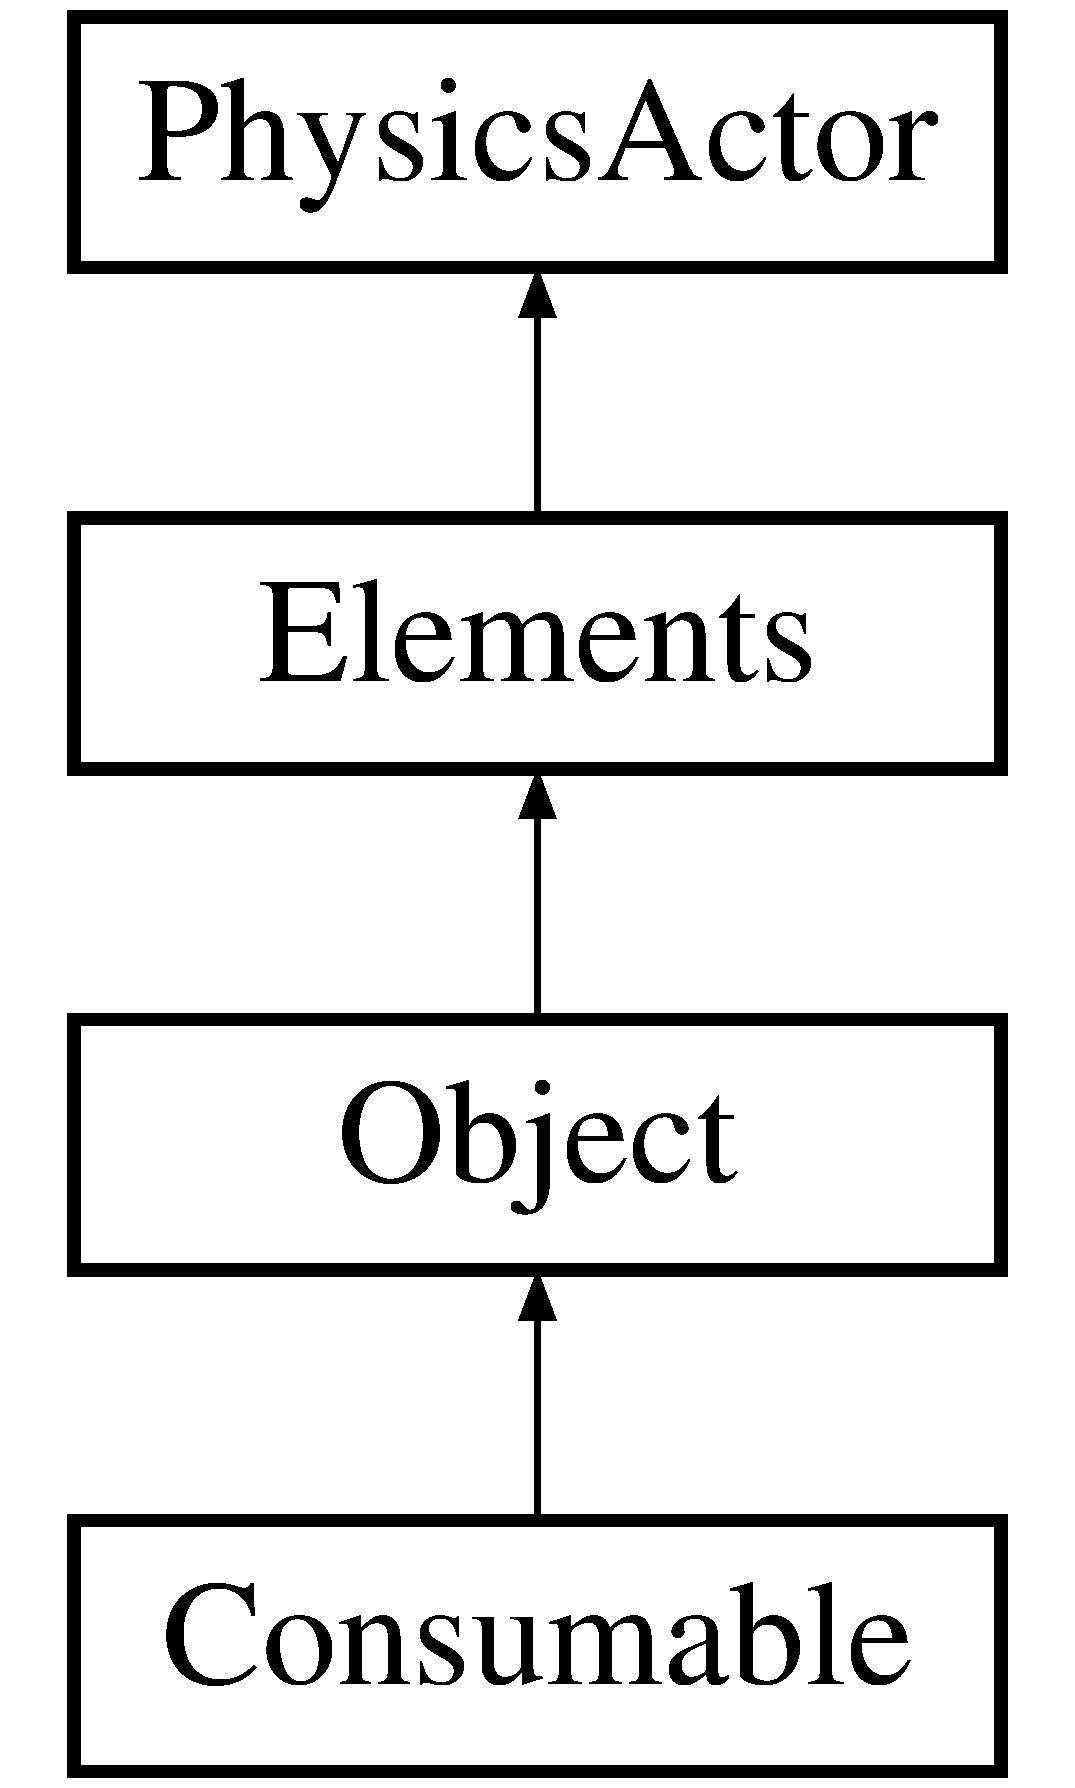
\includegraphics[height=4.000000cm]{class_consumable}
\end{center}
\end{figure}
\subsection*{Public Member Functions}
\begin{DoxyCompactItemize}
\item 
\hyperlink{class_consumable_ae374944f6333618dd08318b98b6950c7}{Consumable} ()
\begin{DoxyCompactList}\small\item\em Basic Constructor. \end{DoxyCompactList}\item 
\hyperlink{class_consumable_adf76e58745007421a38fb07af1c35d1a}{Consumable} (std\+::string type, std\+::string value, \hyperlink{class_characters}{Characters} $\ast$c)
\begin{DoxyCompactList}\small\item\em Third override, used to create consumable based on a Characters$\ast$ position) \end{DoxyCompactList}\item 
\hyperlink{class_consumable_adeca9f0d06a24fb2b76ddaa1396d1ddc}{Consumable} (\hyperlink{class_characters}{Characters} $\ast$c)
\begin{DoxyCompactList}\small\item\em Constructor overriding. \end{DoxyCompactList}\item 
\hypertarget{class_consumable_aed7671d58f80f5244e5851f591e4b8a2}{\hyperlink{class_consumable_aed7671d58f80f5244e5851f591e4b8a2}{$\sim$\+Consumable} ()}\label{class_consumable_aed7671d58f80f5244e5851f591e4b8a2}

\begin{DoxyCompactList}\small\item\em Destructor. \end{DoxyCompactList}\item 
void \hyperlink{class_consumable_adb866e69c3796edffad832b88e527518}{Begin\+Contact} (\hyperlink{class_elements}{Elements} $\ast$elem, b2\+Contact $\ast$contact)
\begin{DoxyCompactList}\small\item\em Collision begin callback. \end{DoxyCompactList}\end{DoxyCompactItemize}
\subsection*{Additional Inherited Members}


\subsection{Detailed Description}
Licensed to the Apache Software Foundation (A\+S\+F) under one or more contributor license agreements. See the N\+O\+T\+I\+C\+E file distributed with this work for additional information regarding copyright ownership. The A\+S\+F licenses this file to you under the Apache License, Version 2.\+0 (the \char`\"{}\+License\char`\"{}); you may not use this file except in compliance with the License. You may obtain a copy of the License at

\href{http://www.apache.org/licenses/LICENSE-2.0}{\tt http\+://www.\+apache.\+org/licenses/\+L\+I\+C\+E\+N\+S\+E-\/2.\+0}

Unless required by applicable law or agreed to in writing, software distributed under the License is distributed on an \char`\"{}\+A\+S I\+S\char`\"{} B\+A\+S\+I\+S, W\+I\+T\+H\+O\+U\+T W\+A\+R\+R\+A\+N\+T\+I\+E\+S O\+R C\+O\+N\+D\+I\+T\+I\+O\+N\+S O\+F A\+N\+Y K\+I\+N\+D, either express or implied. See the License for the specific language governing permissions and limitations under the License. File\+: \hyperlink{_consumable_8hpp_source}{Consumable.\+hpp} Creation\+: 2015-\/03-\/06 15\+:39 Manon Budin \href{mailto:mbudin@student.42.fr}{\tt mbudin@student.\+42.\+fr} 

\subsection{Constructor \& Destructor Documentation}
\hypertarget{class_consumable_ae374944f6333618dd08318b98b6950c7}{\index{Consumable@{Consumable}!Consumable@{Consumable}}
\index{Consumable@{Consumable}!Consumable@{Consumable}}
\subsubsection[{Consumable}]{\setlength{\rightskip}{0pt plus 5cm}Consumable\+::\+Consumable (
\begin{DoxyParamCaption}
\item[{void}]{}
\end{DoxyParamCaption}
)}}\label{class_consumable_ae374944f6333618dd08318b98b6950c7}


Basic Constructor. 

Licensed to the Apache Software Foundation (A\+S\+F) under one or more contributor license agreements. See the N\+O\+T\+I\+C\+E file distributed with this work for additional information regarding copyright ownership. The A\+S\+F licenses this file to you under the Apache License, Version 2.\+0 (the \char`\"{}\+License\char`\"{}); you may not use this file except in compliance with the License. You may obtain a copy of the License at

\href{http://www.apache.org/licenses/LICENSE-2.0}{\tt http\+://www.\+apache.\+org/licenses/\+L\+I\+C\+E\+N\+S\+E-\/2.\+0}

Unless required by applicable law or agreed to in writing, software distributed under the License is distributed on an \char`\"{}\+A\+S I\+S\char`\"{} B\+A\+S\+I\+S, W\+I\+T\+H\+O\+U\+T W\+A\+R\+R\+A\+N\+T\+I\+E\+S O\+R C\+O\+N\+D\+I\+T\+I\+O\+N\+S O\+F A\+N\+Y K\+I\+N\+D, either express or implied. See the License for the specific language governing permissions and limitations under the License. File\+: Consumable.\+cpp Creation\+: 2015-\/03-\/06 15\+:37 Manon Budin \href{mailto:mbudin@student.42.fr}{\tt mbudin@student.\+42.\+fr} Basic Constructor This constructor sets a lots of attributes, like the sprite, the position. etc... That also init the physics. \begin{DoxyRefDesc}{Todo}
\item[\hyperlink{todo__todo000004}{Todo}]This function setting attributes the hard-\/way. Maybe a name based config, like \hyperlink{class_characters}{Characters}, would be better ? \end{DoxyRefDesc}
\hypertarget{class_consumable_adf76e58745007421a38fb07af1c35d1a}{\index{Consumable@{Consumable}!Consumable@{Consumable}}
\index{Consumable@{Consumable}!Consumable@{Consumable}}
\subsubsection[{Consumable}]{\setlength{\rightskip}{0pt plus 5cm}Consumable\+::\+Consumable (
\begin{DoxyParamCaption}
\item[{std\+::string}]{type, }
\item[{std\+::string}]{value, }
\item[{{\bf Characters} $\ast$}]{c}
\end{DoxyParamCaption}
)}}\label{class_consumable_adf76e58745007421a38fb07af1c35d1a}


Third override, used to create consumable based on a Characters$\ast$ position) 

Mostly called for looting, after the death of a mob 
\begin{DoxyParams}{Parameters}
{\em type} & -\/ gold/hp \\
\hline
{\em value} & -\/ how much \\
\hline
{\em c} & -\/ the Character, for the position and such \\
\hline
\end{DoxyParams}
\hypertarget{class_consumable_adeca9f0d06a24fb2b76ddaa1396d1ddc}{\index{Consumable@{Consumable}!Consumable@{Consumable}}
\index{Consumable@{Consumable}!Consumable@{Consumable}}
\subsubsection[{Consumable}]{\setlength{\rightskip}{0pt plus 5cm}Consumable\+::\+Consumable (
\begin{DoxyParamCaption}
\item[{{\bf Characters} $\ast$}]{c}
\end{DoxyParamCaption}
)}}\label{class_consumable_adeca9f0d06a24fb2b76ddaa1396d1ddc}


Constructor overriding. 

Basic Constructor This constructor sets a lots of attributes, like the sprite, the position. etc... That also init the physics. This constructor will use the infos contained in enemy in order to set the different infos in it \begin{DoxyRefDesc}{Todo}
\item[\hyperlink{todo__todo000005}{Todo}]This function setting attributes the hard-\/way. Maybe a name based config, like \hyperlink{class_characters}{Characters}, would be better ? \end{DoxyRefDesc}


\subsection{Member Function Documentation}
\hypertarget{class_consumable_adb866e69c3796edffad832b88e527518}{\index{Consumable@{Consumable}!Begin\+Contact@{Begin\+Contact}}
\index{Begin\+Contact@{Begin\+Contact}!Consumable@{Consumable}}
\subsubsection[{Begin\+Contact}]{\setlength{\rightskip}{0pt plus 5cm}void Consumable\+::\+Begin\+Contact (
\begin{DoxyParamCaption}
\item[{{\bf Elements} $\ast$}]{elem, }
\item[{b2\+Contact $\ast$}]{contact}
\end{DoxyParamCaption}
)\hspace{0.3cm}{\ttfamily [virtual]}}}\label{class_consumable_adb866e69c3796edffad832b88e527518}


Collision begin callback. 

Collision begin function /!\textbackslash{} This function is called just before a collision 
\begin{DoxyParams}{Parameters}
{\em } & elem The \hyperlink{class_elements}{Elements} who collide. \\
\hline
{\em } & contact The Box2\+D contact object. See Box2\+D docs for more information. \\
\hline
\end{DoxyParams}
\begin{DoxyRefDesc}{Todo}
\item[\hyperlink{todo__todo000006}{Todo}]This function is actually doing nothing. \end{DoxyRefDesc}


Reimplemented from \hyperlink{class_elements}{Elements}.



The documentation for this class was generated from the following files\+:\begin{DoxyCompactItemize}
\item 
Sources/inc/Consumable.\+hpp\item 
Sources/src/Consumable.\+cpp\end{DoxyCompactItemize}

\hypertarget{class_contact_filter}{\section{Contact\-Filter Class Reference}
\label{class_contact_filter}\index{Contact\-Filter@{Contact\-Filter}}
}


{\ttfamily \#include $<$Contact\-Filter.\-hpp$>$}



Inheritance diagram for Contact\-Filter\-:
\nopagebreak
\begin{figure}[H]
\begin{center}
\leavevmode
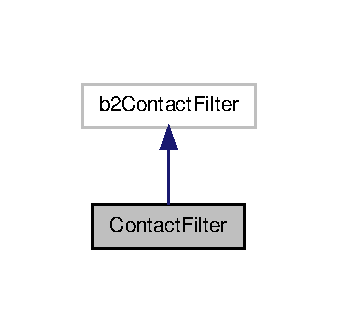
\includegraphics[width=162pt]{class_contact_filter__inherit__graph}
\end{center}
\end{figure}


Collaboration diagram for Contact\-Filter\-:
\nopagebreak
\begin{figure}[H]
\begin{center}
\leavevmode
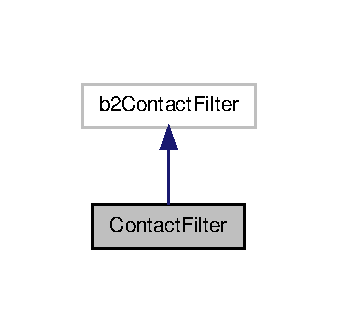
\includegraphics[width=162pt]{class_contact_filter__coll__graph}
\end{center}
\end{figure}
\subsection*{Public Member Functions}
\begin{DoxyCompactItemize}
\item 
bool \hyperlink{class_contact_filter_aa1f43a83fda36c0d4e0479e370350585}{Should\-Collide} (b2\-Fixture $\ast$a, b2\-Fixture $\ast$\hyperlink{jquery_8js_a2fa551895933fae935a0a6b87282241d}{b})
\end{DoxyCompactItemize}


\subsection{Detailed Description}
Licensed to the Apache Software Foundation (A\-S\-F) under one or more contributor license agreements. See the N\-O\-T\-I\-C\-E file distributed with this work for additional information regarding copyright ownership. The A\-S\-F licenses this file to you under the Apache License, Version 2.\-0 (the \char`\"{}\-License\char`\"{}); you may not use this file except in compliance with the License. You may obtain a copy of the License at

\href{http://www.apache.org/licenses/LICENSE-2.0}{\tt http\-://www.\-apache.\-org/licenses/\-L\-I\-C\-E\-N\-S\-E-\/2.\-0}

Unless required by applicable law or agreed to in writing, software distributed under the License is distributed on an \char`\"{}\-A\-S I\-S\char`\"{} B\-A\-S\-I\-S, W\-I\-T\-H\-O\-U\-T W\-A\-R\-R\-A\-N\-T\-I\-E\-S O\-R C\-O\-N\-D\-I\-T\-I\-O\-N\-S O\-F A\-N\-Y K\-I\-N\-D, either express or implied. See the License for the specific language governing permissions and limitations under the License. File\-: \hyperlink{_contact_filter_8cpp}{Contact\-Filter.\-cpp} Creation\-: 2015-\/02-\/23 12\-:40 Vincent Rey \href{mailto:vrey@student.42.fr}{\tt vrey@student.\-42.\-fr} 

\subsection{Member Function Documentation}
\hypertarget{class_contact_filter_aa1f43a83fda36c0d4e0479e370350585}{\index{Contact\-Filter@{Contact\-Filter}!Should\-Collide@{Should\-Collide}}
\index{Should\-Collide@{Should\-Collide}!ContactFilter@{Contact\-Filter}}
\subsubsection[{Should\-Collide}]{\setlength{\rightskip}{0pt plus 5cm}bool Contact\-Filter\-::\-Should\-Collide (
\begin{DoxyParamCaption}
\item[{b2\-Fixture $\ast$}]{fix\-A, }
\item[{b2\-Fixture $\ast$}]{fix\-B}
\end{DoxyParamCaption}
)}}\label{class_contact_filter_aa1f43a83fda36c0d4e0479e370350585}
Licensed to the Apache Software Foundation (A\-S\-F) under one or more contributor license agreements. See the N\-O\-T\-I\-C\-E file distributed with this work for additional information regarding copyright ownership. The A\-S\-F licenses this file to you under the Apache License, Version 2.\-0 (the \char`\"{}\-License\char`\"{}); you may not use this file except in compliance with the License. You may obtain a copy of the License at

\href{http://www.apache.org/licenses/LICENSE-2.0}{\tt http\-://www.\-apache.\-org/licenses/\-L\-I\-C\-E\-N\-S\-E-\/2.\-0}

Unless required by applicable law or agreed to in writing, software distributed under the License is distributed on an \char`\"{}\-A\-S I\-S\char`\"{} B\-A\-S\-I\-S, W\-I\-T\-H\-O\-U\-T W\-A\-R\-R\-A\-N\-T\-I\-E\-S O\-R C\-O\-N\-D\-I\-T\-I\-O\-N\-S O\-F A\-N\-Y K\-I\-N\-D, either express or implied. See the License for the specific language governing permissions and limitations under the License. File\-: \hyperlink{_contact_filter_8hpp}{Contact\-Filter.\-hpp} Creation\-: 2015-\/02-\/23 12\-:40 Vincent Rey \href{mailto:vrey@student.42.fr}{\tt vrey@student.\-42.\-fr} 

The documentation for this class was generated from the following files\-:\begin{DoxyCompactItemize}
\item 
/home/louis/\-Documents/rogue-\/like/\-Sources/inc/\hyperlink{_contact_filter_8hpp}{Contact\-Filter.\-hpp}\item 
/home/louis/\-Documents/rogue-\/like/\-Sources/src/\hyperlink{_contact_filter_8cpp}{Contact\-Filter.\-cpp}\end{DoxyCompactItemize}

\hypertarget{class_elements}{\section{Elements Class Reference}
\label{class_elements}\index{Elements@{Elements}}
}


{\ttfamily \#include $<$Elements.\-hpp$>$}



Inheritance diagram for Elements\-:
\nopagebreak
\begin{figure}[H]
\begin{center}
\leavevmode
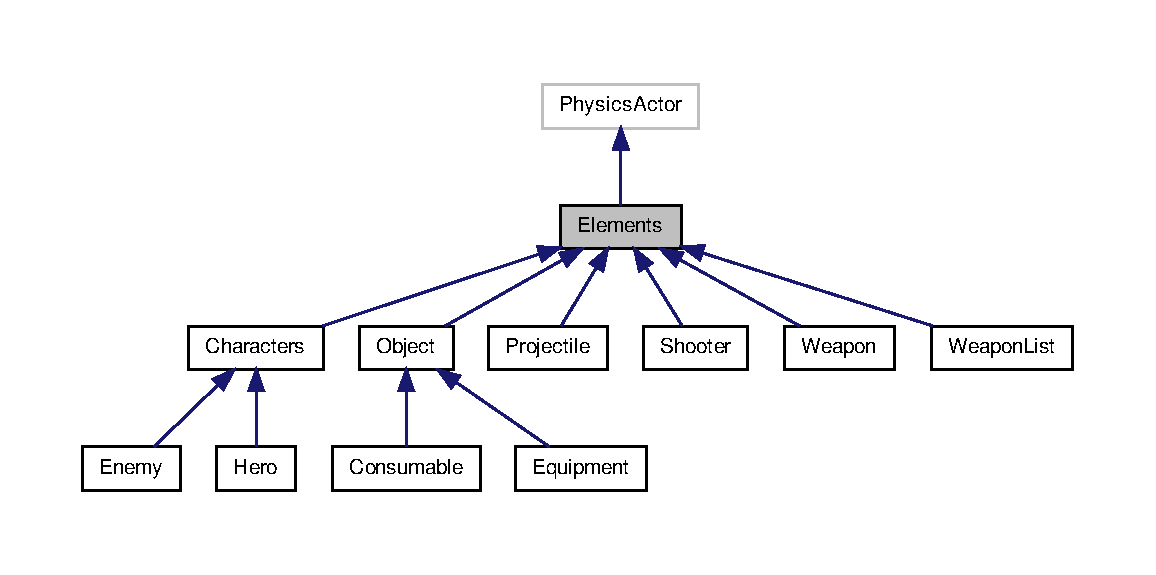
\includegraphics[width=350pt]{class_elements__inherit__graph}
\end{center}
\end{figure}


Collaboration diagram for Elements\-:
\nopagebreak
\begin{figure}[H]
\begin{center}
\leavevmode
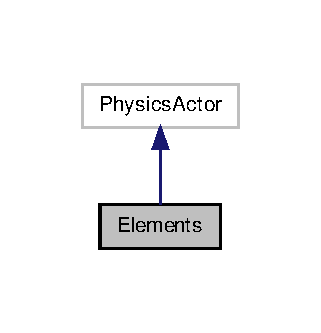
\includegraphics[width=154pt]{class_elements__coll__graph}
\end{center}
\end{figure}
\subsection*{Public Member Functions}
\begin{DoxyCompactItemize}
\item 
\hyperlink{class_elements_aaf76c70282b6997fc20f1d8c751d7146}{Elements} ()
\begin{DoxyCompactList}\small\item\em Base constructor. \end{DoxyCompactList}\item 
\hyperlink{class_elements_a15505a7088b59b169943cf0b3883d859}{Elements} (int id)
\begin{DoxyCompactList}\small\item\em Main constructor. \end{DoxyCompactList}\item 
\hyperlink{class_elements_a2a0658f7634191593c7d6eeab1556adc}{Elements} (\hyperlink{class_elements}{Elements} \&obj)
\begin{DoxyCompactList}\small\item\em Copy constructor. \end{DoxyCompactList}\item 
\hyperlink{class_elements_a28037b21a12317e69d6160da9f4844de}{$\sim$\-Elements} ()
\begin{DoxyCompactList}\small\item\em Basic destructor. \end{DoxyCompactList}\item 
void \hyperlink{class_elements_a23add0eda070fb51f84eab6b94d5b886}{set\-X\-Start} (float X)
\item 
void \hyperlink{class_elements_a2214c37dc1288a3763db6780bf7d6ee5}{set\-Y\-Start} (float Y)
\item 
void \hyperlink{class_elements_a16f6accfe5a20c996dae8154132e4bf7}{set\-Width} (int w)
\item 
void \hyperlink{class_elements_ad778acde74a8640958c6db2b7dd782bc}{set\-Height} (int h)
\item 
void \hyperlink{class_elements_ad82fc7032101163c452a9469a095acab}{set\-Cut\-Width} (int w)
\item 
void \hyperlink{class_elements_a58ffc59bb3226e252ca50bdc67db46b5}{set\-Cut\-Height} (int h)
\item 
void \hyperlink{class_elements_a9ba8c94a6f92d510d60b51239a42b67c}{set\-Frame} (int n)
\item 
void \hyperlink{class_elements_a4aac83563af945cf6c05af4e4d6a173b}{add\-Attribute} (std\-::string name, std\-::string value)
\begin{DoxyCompactList}\small\item\em Add an attribute. \end{DoxyCompactList}\item 
std\-::string \hyperlink{class_elements_ab35a8e49a075adca1dee3e941865e20f}{get\-Attribute} (std\-::string name)
\begin{DoxyCompactList}\small\item\em A getter for attribute. \end{DoxyCompactList}\item 
void \hyperlink{class_elements_ae549e0c8599f06b42126c67c5dd68fd2}{remove\-Attr} (std\-::string name)
\begin{DoxyCompactList}\small\item\em Remove an attribute. \end{DoxyCompactList}\item 
void \hyperlink{class_elements_adeca7401d8bc32fa75e2c2a0b2627412}{display} (void)
\begin{DoxyCompactList}\small\item\em Display an element. \end{DoxyCompactList}\item 
std\-::map$<$ std\-::string, \\*
std\-::string $>$ \hyperlink{class_elements_aff6b1b8c11e8579384461eadc63ee39e}{get\-Attributes} (void)
\item 
void \hyperlink{class_elements_a3bb4cc2e2009d0e447fbdd0212a57b73}{set\-Frame\-Sprite} (int frame)
\begin{DoxyCompactList}\small\item\em Set frame in a sprite\-File. \end{DoxyCompactList}\item 
void \hyperlink{class_elements_ad7e4ecb2ecc2402cf892e60d8d803070}{set\-Hitbox} (std\-::string)
\item 
virtual void \hyperlink{class_elements_a85bc66fe037551fcfa0b606cf32c4478}{callback} (\hyperlink{class_elements}{Elements} $\ast$elem)
\item 
virtual void \hyperlink{class_elements_a108938e08197adc349e98fb91abe1b5a}{Begin\-Contact} (\hyperlink{class_elements}{Elements} $\ast$elem, b2\-Contact $\ast$contact)
\item 
virtual void \hyperlink{class_elements_a42c3b694edefcc789109bd952a66d918}{End\-Contact} (\hyperlink{class_elements}{Elements} $\ast$elem, b2\-Contact $\ast$contact)
\item 
int \hyperlink{class_elements_a2dd2e1e757c9077755bbe309c504740b}{get\-Orientation\-X} (void)
\item 
int \hyperlink{class_elements_a58d9facbd7f6264e8b4e2ff49f20d939}{get\-Orientation\-Y} (void)
\item 
int \hyperlink{class_elements_add4340c523571631da317d8a64fc1368}{get\-Lateral\-Orientation} (void)
\end{DoxyCompactItemize}
\subsection*{Protected Member Functions}
\begin{DoxyCompactItemize}
\item 
virtual void \hyperlink{class_elements_aa367c1471a9fc7f1a9b7b124e69c3ef3}{\-\_\-run} ()
\end{DoxyCompactItemize}
\subsection*{Protected Attributes}
\begin{DoxyCompactItemize}
\item 
std\-::string \hyperlink{class_elements_a8968fcb76f2c8473b2715415ddc2d8be}{\-\_\-hitbox\-Type}
\item 
std\-::string \hyperlink{class_elements_a7e38d955602d5ea837411a6ffcb0d2cd}{\-\_\-hitbox}
\end{DoxyCompactItemize}
\subsection*{Friends}
\begin{DoxyCompactItemize}
\item 
class \hyperlink{class_elements_aa2fab026580d6f14280c2ffb8063a314}{Game}
\end{DoxyCompactItemize}


\subsection{Constructor \& Destructor Documentation}
\hypertarget{class_elements_aaf76c70282b6997fc20f1d8c751d7146}{\index{Elements@{Elements}!Elements@{Elements}}
\index{Elements@{Elements}!Elements@{Elements}}
\subsubsection[{Elements}]{\setlength{\rightskip}{0pt plus 5cm}Elements\-::\-Elements (
\begin{DoxyParamCaption}
\item[{void}]{}
\end{DoxyParamCaption}
)}}\label{class_elements_aaf76c70282b6997fc20f1d8c751d7146}


Base constructor. 

\hypertarget{class_elements_a15505a7088b59b169943cf0b3883d859}{\index{Elements@{Elements}!Elements@{Elements}}
\index{Elements@{Elements}!Elements@{Elements}}
\subsubsection[{Elements}]{\setlength{\rightskip}{0pt plus 5cm}Elements\-::\-Elements (
\begin{DoxyParamCaption}
\item[{int}]{id}
\end{DoxyParamCaption}
)}}\label{class_elements_a15505a7088b59b169943cf0b3883d859}


Main constructor. 

Licensed to the Apache Software Foundation (A\-S\-F) under one or more contributor license agreements. See the N\-O\-T\-I\-C\-E file distributed with this work for additional information regarding copyright ownership. The A\-S\-F licenses this file to you under the Apache License, Version 2.\-0 (the \char`\"{}\-License\char`\"{}); you may not use this file except in compliance with the License. You may obtain a copy of the License at

\href{http://www.apache.org/licenses/LICENSE-2.0}{\tt http\-://www.\-apache.\-org/licenses/\-L\-I\-C\-E\-N\-S\-E-\/2.\-0}

Unless required by applicable law or agreed to in writing, software distributed under the License is distributed on an \char`\"{}\-A\-S I\-S\char`\"{} B\-A\-S\-I\-S, W\-I\-T\-H\-O\-U\-T W\-A\-R\-R\-A\-N\-T\-I\-E\-S O\-R C\-O\-N\-D\-I\-T\-I\-O\-N\-S O\-F A\-N\-Y K\-I\-N\-D, either express or implied. See the License for the specific language governing permissions and limitations under the License. File\-: \hyperlink{_elements_8cpp}{Elements.\-cpp} \begin{DoxyDate}{Date}
2015-\/02-\/13 07\-:39 
\end{DoxyDate}
\begin{DoxyAuthor}{Author}
Louis Solofrizzo \href{mailto:louis@ne02ptzero.me}{\tt louis@ne02ptzero.\-me} 
\end{DoxyAuthor}

\begin{DoxyParams}{Parameters}
{\em id} & The future id of the element  This function is outdated due to recent changes in the A\-P\-I. \\
\hline
\end{DoxyParams}
\hypertarget{class_elements_a2a0658f7634191593c7d6eeab1556adc}{\index{Elements@{Elements}!Elements@{Elements}}
\index{Elements@{Elements}!Elements@{Elements}}
\subsubsection[{Elements}]{\setlength{\rightskip}{0pt plus 5cm}Elements\-::\-Elements (
\begin{DoxyParamCaption}
\item[{{\bf Elements} \&}]{obj}
\end{DoxyParamCaption}
)}}\label{class_elements_a2a0658f7634191593c7d6eeab1556adc}


Copy constructor. 

The constructor by Copy, thank's to the Coplien's form. 
\begin{DoxyParams}{Parameters}
{\em obj} & The object we have to copy. \\
\hline
\end{DoxyParams}
\hypertarget{class_elements_a28037b21a12317e69d6160da9f4844de}{\index{Elements@{Elements}!$\sim$\-Elements@{$\sim$\-Elements}}
\index{$\sim$\-Elements@{$\sim$\-Elements}!Elements@{Elements}}
\subsubsection[{$\sim$\-Elements}]{\setlength{\rightskip}{0pt plus 5cm}Elements\-::$\sim$\-Elements (
\begin{DoxyParamCaption}
\item[{void}]{}
\end{DoxyParamCaption}
)}}\label{class_elements_a28037b21a12317e69d6160da9f4844de}


Basic destructor. 



\subsection{Member Function Documentation}
\hypertarget{class_elements_aa367c1471a9fc7f1a9b7b124e69c3ef3}{\index{Elements@{Elements}!\-\_\-run@{\-\_\-run}}
\index{\-\_\-run@{\-\_\-run}!Elements@{Elements}}
\subsubsection[{\-\_\-run}]{\setlength{\rightskip}{0pt plus 5cm}virtual void Elements\-::\-\_\-run (
\begin{DoxyParamCaption}
\item[{void}]{}
\end{DoxyParamCaption}
)\hspace{0.3cm}{\ttfamily [inline]}, {\ttfamily [protected]}, {\ttfamily [virtual]}}}\label{class_elements_aa367c1471a9fc7f1a9b7b124e69c3ef3}


Reimplemented in \hyperlink{class_characters_aa59e298bef3e58fc7c82deb86e762200}{Characters}.

\hypertarget{class_elements_a4aac83563af945cf6c05af4e4d6a173b}{\index{Elements@{Elements}!add\-Attribute@{add\-Attribute}}
\index{add\-Attribute@{add\-Attribute}!Elements@{Elements}}
\subsubsection[{add\-Attribute}]{\setlength{\rightskip}{0pt plus 5cm}void Elements\-::add\-Attribute (
\begin{DoxyParamCaption}
\item[{std\-::string}]{name, }
\item[{std\-::string}]{value}
\end{DoxyParamCaption}
)}}\label{class_elements_a4aac83563af945cf6c05af4e4d6a173b}


Add an attribute. 

Add an attribute to the Element 
\begin{DoxyParams}{Parameters}
{\em name} & Name of the attribute \\
\hline
{\em value} & Value of the attribute  This method of attribute is outdated due to the new Json\-::\-Value politic in the A\-P\-I, more flexible. \\
\hline
\end{DoxyParams}
\hypertarget{class_elements_a108938e08197adc349e98fb91abe1b5a}{\index{Elements@{Elements}!Begin\-Contact@{Begin\-Contact}}
\index{Begin\-Contact@{Begin\-Contact}!Elements@{Elements}}
\subsubsection[{Begin\-Contact}]{\setlength{\rightskip}{0pt plus 5cm}virtual void Elements\-::\-Begin\-Contact (
\begin{DoxyParamCaption}
\item[{{\bf Elements} $\ast$}]{elem, }
\item[{b2\-Contact $\ast$}]{contact}
\end{DoxyParamCaption}
)\hspace{0.3cm}{\ttfamily [inline]}, {\ttfamily [virtual]}}}\label{class_elements_a108938e08197adc349e98fb91abe1b5a}


Reimplemented in \hyperlink{class_characters_ae1b52f35e60cd23ec118595a9a8e8760}{Characters}, \hyperlink{class_projectile_a7347375e9c8cae921709ba56265af0fd}{Projectile}, \hyperlink{class_weapon_a866884395ed4c0e7a972bb18e8d7d030}{Weapon}, \hyperlink{class_enemy_a3938e3e2cf5f07d809e1f1927b09539a}{Enemy}, \hyperlink{class_equipment_a0c706b45578e8d01fec7b8ee1b773987}{Equipment}, \hyperlink{class_consumable_adb866e69c3796edffad832b88e527518}{Consumable}, \hyperlink{class_hero_ac23c090d8f5e2768b4175580a0d53d1b}{Hero}, and \hyperlink{class_object_a5681745b50d64994e00fe519bbb4cd31}{Object}.

\hypertarget{class_elements_a85bc66fe037551fcfa0b606cf32c4478}{\index{Elements@{Elements}!callback@{callback}}
\index{callback@{callback}!Elements@{Elements}}
\subsubsection[{callback}]{\setlength{\rightskip}{0pt plus 5cm}virtual void Elements\-::callback (
\begin{DoxyParamCaption}
\item[{{\bf Elements} $\ast$}]{elem}
\end{DoxyParamCaption}
)\hspace{0.3cm}{\ttfamily [inline]}, {\ttfamily [virtual]}}}\label{class_elements_a85bc66fe037551fcfa0b606cf32c4478}
\hypertarget{class_elements_adeca7401d8bc32fa75e2c2a0b2627412}{\index{Elements@{Elements}!display@{display}}
\index{display@{display}!Elements@{Elements}}
\subsubsection[{display}]{\setlength{\rightskip}{0pt plus 5cm}void Elements\-::display (
\begin{DoxyParamCaption}
\item[{void}]{}
\end{DoxyParamCaption}
)}}\label{class_elements_adeca7401d8bc32fa75e2c2a0b2627412}


Display an element. 

Load physics on element, and add him to the World.  This function is quite nasty, maybe a rework on it should be better. \hypertarget{class_elements_a42c3b694edefcc789109bd952a66d918}{\index{Elements@{Elements}!End\-Contact@{End\-Contact}}
\index{End\-Contact@{End\-Contact}!Elements@{Elements}}
\subsubsection[{End\-Contact}]{\setlength{\rightskip}{0pt plus 5cm}virtual void Elements\-::\-End\-Contact (
\begin{DoxyParamCaption}
\item[{{\bf Elements} $\ast$}]{elem, }
\item[{b2\-Contact $\ast$}]{contact}
\end{DoxyParamCaption}
)\hspace{0.3cm}{\ttfamily [inline]}, {\ttfamily [virtual]}}}\label{class_elements_a42c3b694edefcc789109bd952a66d918}


Reimplemented in \hyperlink{class_characters_a87c76bb34f5c11e2da4537be07d2f846}{Characters}, \hyperlink{class_projectile_a9f8fa9403a414fa1fd6ee092720ca4e6}{Projectile}, \hyperlink{class_weapon_a1860f840f8c75555de52450300139d9b}{Weapon}, \hyperlink{class_equipment_abda1acd976a1c33f3aa398b3a9a64555}{Equipment}, and \hyperlink{class_hero_a9fee92d1b0df478f95bc10ba84015d2a}{Hero}.

\hypertarget{class_elements_ab35a8e49a075adca1dee3e941865e20f}{\index{Elements@{Elements}!get\-Attribute@{get\-Attribute}}
\index{get\-Attribute@{get\-Attribute}!Elements@{Elements}}
\subsubsection[{get\-Attribute}]{\setlength{\rightskip}{0pt plus 5cm}std\-::string Elements\-::get\-Attribute (
\begin{DoxyParamCaption}
\item[{std\-::string}]{name}
\end{DoxyParamCaption}
)}}\label{class_elements_ab35a8e49a075adca1dee3e941865e20f}


A getter for attribute. 

Get an attribute value 
\begin{DoxyParams}{Parameters}
{\em name} & The Name of the attribute \\
\hline
\end{DoxyParams}
\begin{DoxyReturn}{Returns}
The value of attribute if found, else \char`\"{}\char`\"{} 
\end{DoxyReturn}
\hypertarget{class_elements_aff6b1b8c11e8579384461eadc63ee39e}{\index{Elements@{Elements}!get\-Attributes@{get\-Attributes}}
\index{get\-Attributes@{get\-Attributes}!Elements@{Elements}}
\subsubsection[{get\-Attributes}]{\setlength{\rightskip}{0pt plus 5cm}std\-::map$<$ std\-::string, std\-::string $>$ Elements\-::get\-Attributes (
\begin{DoxyParamCaption}
\item[{void}]{}
\end{DoxyParamCaption}
)}}\label{class_elements_aff6b1b8c11e8579384461eadc63ee39e}
\hypertarget{class_elements_add4340c523571631da317d8a64fc1368}{\index{Elements@{Elements}!get\-Lateral\-Orientation@{get\-Lateral\-Orientation}}
\index{get\-Lateral\-Orientation@{get\-Lateral\-Orientation}!Elements@{Elements}}
\subsubsection[{get\-Lateral\-Orientation}]{\setlength{\rightskip}{0pt plus 5cm}int Elements\-::get\-Lateral\-Orientation (
\begin{DoxyParamCaption}
\item[{void}]{}
\end{DoxyParamCaption}
)}}\label{class_elements_add4340c523571631da317d8a64fc1368}
\hypertarget{class_elements_a2dd2e1e757c9077755bbe309c504740b}{\index{Elements@{Elements}!get\-Orientation\-X@{get\-Orientation\-X}}
\index{get\-Orientation\-X@{get\-Orientation\-X}!Elements@{Elements}}
\subsubsection[{get\-Orientation\-X}]{\setlength{\rightskip}{0pt plus 5cm}int Elements\-::get\-Orientation\-X (
\begin{DoxyParamCaption}
\item[{void}]{}
\end{DoxyParamCaption}
)}}\label{class_elements_a2dd2e1e757c9077755bbe309c504740b}
\hypertarget{class_elements_a58d9facbd7f6264e8b4e2ff49f20d939}{\index{Elements@{Elements}!get\-Orientation\-Y@{get\-Orientation\-Y}}
\index{get\-Orientation\-Y@{get\-Orientation\-Y}!Elements@{Elements}}
\subsubsection[{get\-Orientation\-Y}]{\setlength{\rightskip}{0pt plus 5cm}int Elements\-::get\-Orientation\-Y (
\begin{DoxyParamCaption}
\item[{void}]{}
\end{DoxyParamCaption}
)}}\label{class_elements_a58d9facbd7f6264e8b4e2ff49f20d939}
\hypertarget{class_elements_ae549e0c8599f06b42126c67c5dd68fd2}{\index{Elements@{Elements}!remove\-Attr@{remove\-Attr}}
\index{remove\-Attr@{remove\-Attr}!Elements@{Elements}}
\subsubsection[{remove\-Attr}]{\setlength{\rightskip}{0pt plus 5cm}void Elements\-::remove\-Attr (
\begin{DoxyParamCaption}
\item[{std\-::string}]{name}
\end{DoxyParamCaption}
)}}\label{class_elements_ae549e0c8599f06b42126c67c5dd68fd2}


Remove an attribute. 

Remove an attribute form the list 
\begin{DoxyParams}{Parameters}
{\em name} & The name of the attribute we have to remove \\
\hline
\end{DoxyParams}
\hypertarget{class_elements_a58ffc59bb3226e252ca50bdc67db46b5}{\index{Elements@{Elements}!set\-Cut\-Height@{set\-Cut\-Height}}
\index{set\-Cut\-Height@{set\-Cut\-Height}!Elements@{Elements}}
\subsubsection[{set\-Cut\-Height}]{\setlength{\rightskip}{0pt plus 5cm}void Elements\-::set\-Cut\-Height (
\begin{DoxyParamCaption}
\item[{int}]{h}
\end{DoxyParamCaption}
)}}\label{class_elements_a58ffc59bb3226e252ca50bdc67db46b5}
\hypertarget{class_elements_ad82fc7032101163c452a9469a095acab}{\index{Elements@{Elements}!set\-Cut\-Width@{set\-Cut\-Width}}
\index{set\-Cut\-Width@{set\-Cut\-Width}!Elements@{Elements}}
\subsubsection[{set\-Cut\-Width}]{\setlength{\rightskip}{0pt plus 5cm}void Elements\-::set\-Cut\-Width (
\begin{DoxyParamCaption}
\item[{int}]{w}
\end{DoxyParamCaption}
)}}\label{class_elements_ad82fc7032101163c452a9469a095acab}
\hypertarget{class_elements_a9ba8c94a6f92d510d60b51239a42b67c}{\index{Elements@{Elements}!set\-Frame@{set\-Frame}}
\index{set\-Frame@{set\-Frame}!Elements@{Elements}}
\subsubsection[{set\-Frame}]{\setlength{\rightskip}{0pt plus 5cm}void Elements\-::set\-Frame (
\begin{DoxyParamCaption}
\item[{int}]{n}
\end{DoxyParamCaption}
)}}\label{class_elements_a9ba8c94a6f92d510d60b51239a42b67c}
\hypertarget{class_elements_a3bb4cc2e2009d0e447fbdd0212a57b73}{\index{Elements@{Elements}!set\-Frame\-Sprite@{set\-Frame\-Sprite}}
\index{set\-Frame\-Sprite@{set\-Frame\-Sprite}!Elements@{Elements}}
\subsubsection[{set\-Frame\-Sprite}]{\setlength{\rightskip}{0pt plus 5cm}void Elements\-::set\-Frame\-Sprite (
\begin{DoxyParamCaption}
\item[{int}]{frame}
\end{DoxyParamCaption}
)}}\label{class_elements_a3bb4cc2e2009d0e447fbdd0212a57b73}


Set frame in a sprite\-File. 

Set a specific frame from a sprite file. This function is currently used only by the the background elements. 
\begin{DoxyParams}{Parameters}
{\em frame} & The frame to display (Reading size left to right)  The height and width of the cutting size is write down in the code (16x16). \\
\hline
\end{DoxyParams}
\hypertarget{class_elements_ad778acde74a8640958c6db2b7dd782bc}{\index{Elements@{Elements}!set\-Height@{set\-Height}}
\index{set\-Height@{set\-Height}!Elements@{Elements}}
\subsubsection[{set\-Height}]{\setlength{\rightskip}{0pt plus 5cm}void Elements\-::set\-Height (
\begin{DoxyParamCaption}
\item[{int}]{h}
\end{DoxyParamCaption}
)}}\label{class_elements_ad778acde74a8640958c6db2b7dd782bc}
\hypertarget{class_elements_ad7e4ecb2ecc2402cf892e60d8d803070}{\index{Elements@{Elements}!set\-Hitbox@{set\-Hitbox}}
\index{set\-Hitbox@{set\-Hitbox}!Elements@{Elements}}
\subsubsection[{set\-Hitbox}]{\setlength{\rightskip}{0pt plus 5cm}void Elements\-::set\-Hitbox (
\begin{DoxyParamCaption}
\item[{std\-::string}]{n}
\end{DoxyParamCaption}
)}}\label{class_elements_ad7e4ecb2ecc2402cf892e60d8d803070}
\hypertarget{class_elements_a16f6accfe5a20c996dae8154132e4bf7}{\index{Elements@{Elements}!set\-Width@{set\-Width}}
\index{set\-Width@{set\-Width}!Elements@{Elements}}
\subsubsection[{set\-Width}]{\setlength{\rightskip}{0pt plus 5cm}void Elements\-::set\-Width (
\begin{DoxyParamCaption}
\item[{int}]{w}
\end{DoxyParamCaption}
)}}\label{class_elements_a16f6accfe5a20c996dae8154132e4bf7}
\hypertarget{class_elements_a23add0eda070fb51f84eab6b94d5b886}{\index{Elements@{Elements}!set\-X\-Start@{set\-X\-Start}}
\index{set\-X\-Start@{set\-X\-Start}!Elements@{Elements}}
\subsubsection[{set\-X\-Start}]{\setlength{\rightskip}{0pt plus 5cm}void Elements\-::set\-X\-Start (
\begin{DoxyParamCaption}
\item[{float}]{X}
\end{DoxyParamCaption}
)}}\label{class_elements_a23add0eda070fb51f84eab6b94d5b886}
\hypertarget{class_elements_a2214c37dc1288a3763db6780bf7d6ee5}{\index{Elements@{Elements}!set\-Y\-Start@{set\-Y\-Start}}
\index{set\-Y\-Start@{set\-Y\-Start}!Elements@{Elements}}
\subsubsection[{set\-Y\-Start}]{\setlength{\rightskip}{0pt plus 5cm}void Elements\-::set\-Y\-Start (
\begin{DoxyParamCaption}
\item[{float}]{Y}
\end{DoxyParamCaption}
)}}\label{class_elements_a2214c37dc1288a3763db6780bf7d6ee5}


\subsection{Friends And Related Function Documentation}
\hypertarget{class_elements_aa2fab026580d6f14280c2ffb8063a314}{\index{Elements@{Elements}!Game@{Game}}
\index{Game@{Game}!Elements@{Elements}}
\subsubsection[{Game}]{\setlength{\rightskip}{0pt plus 5cm}friend class {\bf Game}\hspace{0.3cm}{\ttfamily [friend]}}}\label{class_elements_aa2fab026580d6f14280c2ffb8063a314}


\subsection{Member Data Documentation}
\hypertarget{class_elements_a7e38d955602d5ea837411a6ffcb0d2cd}{\index{Elements@{Elements}!\-\_\-hitbox@{\-\_\-hitbox}}
\index{\-\_\-hitbox@{\-\_\-hitbox}!Elements@{Elements}}
\subsubsection[{\-\_\-hitbox}]{\setlength{\rightskip}{0pt plus 5cm}std\-::string Elements\-::\-\_\-hitbox\hspace{0.3cm}{\ttfamily [protected]}}}\label{class_elements_a7e38d955602d5ea837411a6ffcb0d2cd}
\hypertarget{class_elements_a8968fcb76f2c8473b2715415ddc2d8be}{\index{Elements@{Elements}!\-\_\-hitbox\-Type@{\-\_\-hitbox\-Type}}
\index{\-\_\-hitbox\-Type@{\-\_\-hitbox\-Type}!Elements@{Elements}}
\subsubsection[{\-\_\-hitbox\-Type}]{\setlength{\rightskip}{0pt plus 5cm}std\-::string Elements\-::\-\_\-hitbox\-Type\hspace{0.3cm}{\ttfamily [protected]}}}\label{class_elements_a8968fcb76f2c8473b2715415ddc2d8be}


The documentation for this class was generated from the following files\-:\begin{DoxyCompactItemize}
\item 
/home/louis/\-Documents/rogue-\/like/\-Sources/inc/\hyperlink{_elements_8hpp}{Elements.\-hpp}\item 
/home/louis/\-Documents/rogue-\/like/\-Sources/src/\hyperlink{_elements_8cpp}{Elements.\-cpp}\end{DoxyCompactItemize}

\hypertarget{class_enemy}{\section{Enemy Class Reference}
\label{class_enemy}\index{Enemy@{Enemy}}
}


{\ttfamily \#include $<$Enemy.\+hpp$>$}

Inheritance diagram for Enemy\+:\begin{figure}[H]
\begin{center}
\leavevmode
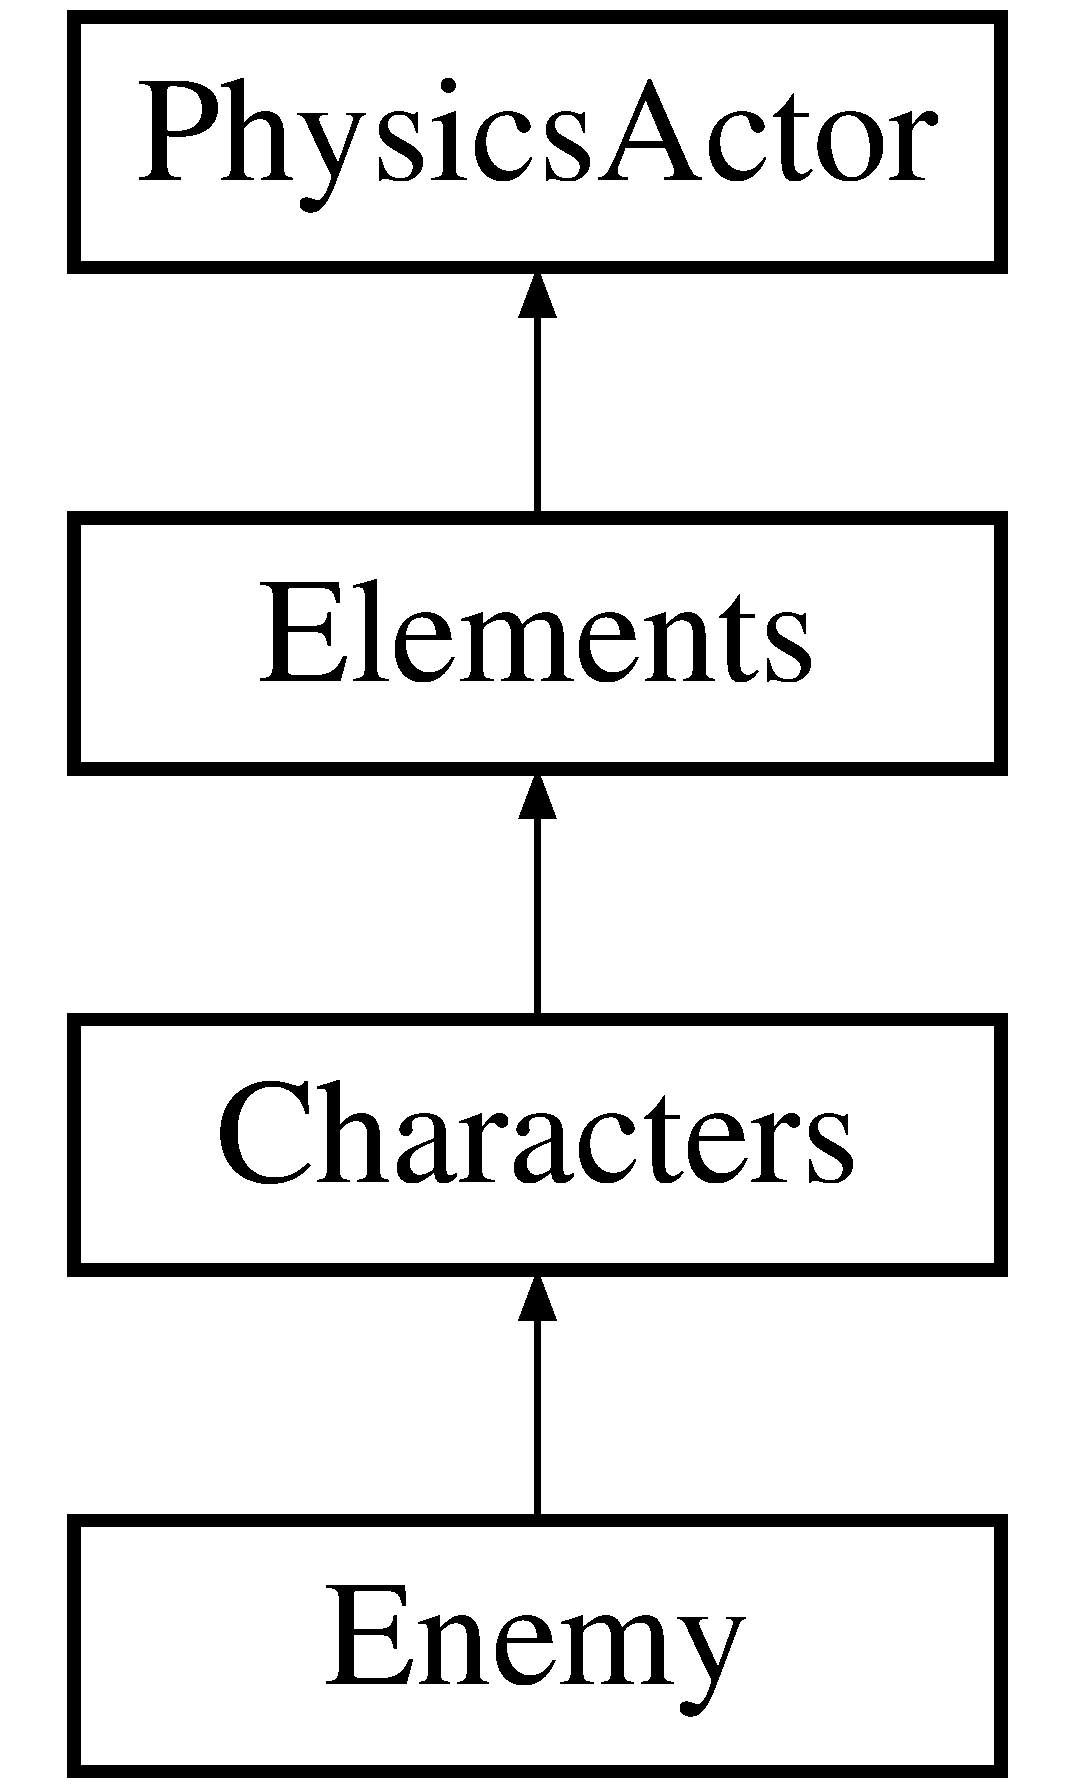
\includegraphics[height=4.000000cm]{class_enemy}
\end{center}
\end{figure}
\subsection*{Public Member Functions}
\begin{DoxyCompactItemize}
\item 
\hyperlink{class_enemy_a94f30d348b6d2840fd71675472ba38dd}{Enemy} ()
\begin{DoxyCompactList}\small\item\em Basic constructor. \end{DoxyCompactList}\item 
\hyperlink{class_enemy_a258ddb71f2f298663dc1ff988dcfd2e2}{Enemy} (std\+::string)
\begin{DoxyCompactList}\small\item\em Main constructor. \end{DoxyCompactList}\item 
\hyperlink{class_enemy_ac0eec4755e28c02688065f9657150ac3}{$\sim$\+Enemy} ()
\begin{DoxyCompactList}\small\item\em Destructor. \end{DoxyCompactList}\item 
int \hyperlink{class_enemy_ae4335909ac929e5e5db7eb01b15fbce8}{take\+Damage} (int damage)
\begin{DoxyCompactList}\small\item\em Take Damage. \end{DoxyCompactList}\item 
void \hyperlink{class_enemy_a2f1157b7c8d74371c2b06493563423ee}{action\+Callback} (std\+::string name, int status)
\begin{DoxyCompactList}\small\item\em Action callback. \end{DoxyCompactList}\item 
void \hyperlink{class_enemy_a4ed496f92f8c791133494d24b4eeaff6}{init} (void)
\begin{DoxyCompactList}\small\item\em Init Animation. \end{DoxyCompactList}\item 
void \hyperlink{class_enemy_a3938e3e2cf5f07d809e1f1927b09539a}{Begin\+Contact} (\hyperlink{class_elements}{Elements} $\ast$m, b2\+Contact $\ast$contact)
\begin{DoxyCompactList}\small\item\em Begin collision function. \end{DoxyCompactList}\end{DoxyCompactItemize}
\subsection*{Additional Inherited Members}


\subsection{Detailed Description}
Licensed to the Apache Software Foundation (A\+S\+F) under one or more contributor license agreements. See the N\+O\+T\+I\+C\+E file distributed with this work for additional information regarding copyright ownership. The A\+S\+F licenses this file to you under the Apache License, Version 2.\+0 (the \char`\"{}\+License\char`\"{}); you may not use this file except in compliance with the License. You may obtain a copy of the License at

\href{http://www.apache.org/licenses/LICENSE-2.0}{\tt http\+://www.\+apache.\+org/licenses/\+L\+I\+C\+E\+N\+S\+E-\/2.\+0}

Unless required by applicable law or agreed to in writing, software distributed under the License is distributed on an \char`\"{}\+A\+S I\+S\char`\"{} B\+A\+S\+I\+S, W\+I\+T\+H\+O\+U\+T W\+A\+R\+R\+A\+N\+T\+I\+E\+S O\+R C\+O\+N\+D\+I\+T\+I\+O\+N\+S O\+F A\+N\+Y K\+I\+N\+D, either express or implied. See the License for the specific language governing permissions and limitations under the License. File\+: \hyperlink{_enemy_8hpp_source}{Enemy.\+hpp} Creation\+: 2015-\/02-\/23 14\+:25 Manon Budin \href{mailto:mbudin@student.42.fr}{\tt mbudin@student.\+42.\+fr} 

\subsection{Constructor \& Destructor Documentation}
\hypertarget{class_enemy_a94f30d348b6d2840fd71675472ba38dd}{\index{Enemy@{Enemy}!Enemy@{Enemy}}
\index{Enemy@{Enemy}!Enemy@{Enemy}}
\subsubsection[{Enemy}]{\setlength{\rightskip}{0pt plus 5cm}Enemy\+::\+Enemy (
\begin{DoxyParamCaption}
\item[{void}]{}
\end{DoxyParamCaption}
)}}\label{class_enemy_a94f30d348b6d2840fd71675472ba38dd}


Basic constructor. 

Licensed to the Apache Software Foundation (A\+S\+F) under one or more contributor license agreements. See the N\+O\+T\+I\+C\+E file distributed with this work for additional information regarding copyright ownership. The A\+S\+F licenses this file to you under the Apache License, Version 2.\+0 (the \char`\"{}\+License\char`\"{}); you may not use this file except in compliance with the License. You may obtain a copy of the License at

\href{http://www.apache.org/licenses/LICENSE-2.0}{\tt http\+://www.\+apache.\+org/licenses/\+L\+I\+C\+E\+N\+S\+E-\/2.\+0}

Unless required by applicable law or agreed to in writing, software distributed under the License is distributed on an \char`\"{}\+A\+S I\+S\char`\"{} B\+A\+S\+I\+S, W\+I\+T\+H\+O\+U\+T W\+A\+R\+R\+A\+N\+T\+I\+E\+S O\+R C\+O\+N\+D\+I\+T\+I\+O\+N\+S O\+F A\+N\+Y K\+I\+N\+D, either express or implied. See the License for the specific language governing permissions and limitations under the License. File\+: Enemy.\+cpp Creation\+: 2015-\/02-\/23 14\+:26 Manon Budin \href{mailto:mbudin@student.42.fr}{\tt mbudin@student.\+42.\+fr} A basic constructor, with an mother (\hyperlink{class_characters}{Characters}) init. \hypertarget{class_enemy_a258ddb71f2f298663dc1ff988dcfd2e2}{\index{Enemy@{Enemy}!Enemy@{Enemy}}
\index{Enemy@{Enemy}!Enemy@{Enemy}}
\subsubsection[{Enemy}]{\setlength{\rightskip}{0pt plus 5cm}Enemy\+::\+Enemy (
\begin{DoxyParamCaption}
\item[{std\+::string}]{str}
\end{DoxyParamCaption}
)}}\label{class_enemy_a258ddb71f2f298663dc1ff988dcfd2e2}


Main constructor. 

The main constructor, init with a name. This constructor set position the hard way, may be better to use the config file info ? 
\begin{DoxyParams}{Parameters}
{\em str} & Name of the new \hyperlink{class_enemy}{Enemy} \\
\hline
\end{DoxyParams}
\hypertarget{class_enemy_ac0eec4755e28c02688065f9657150ac3}{\index{Enemy@{Enemy}!````~Enemy@{$\sim$\+Enemy}}
\index{````~Enemy@{$\sim$\+Enemy}!Enemy@{Enemy}}
\subsubsection[{$\sim$\+Enemy}]{\setlength{\rightskip}{0pt plus 5cm}Enemy\+::$\sim$\+Enemy (
\begin{DoxyParamCaption}
\item[{void}]{}
\end{DoxyParamCaption}
)}}\label{class_enemy_ac0eec4755e28c02688065f9657150ac3}


Destructor. 

Basic Destructor 

\subsection{Member Function Documentation}
\hypertarget{class_enemy_a2f1157b7c8d74371c2b06493563423ee}{\index{Enemy@{Enemy}!action\+Callback@{action\+Callback}}
\index{action\+Callback@{action\+Callback}!Enemy@{Enemy}}
\subsubsection[{action\+Callback}]{\setlength{\rightskip}{0pt plus 5cm}void Enemy\+::action\+Callback (
\begin{DoxyParamCaption}
\item[{std\+::string}]{name, }
\item[{int}]{status}
\end{DoxyParamCaption}
)\hspace{0.3cm}{\ttfamily [virtual]}}}\label{class_enemy_a2f1157b7c8d74371c2b06493563423ee}


Action callback. 

Mother's callback for actions See \hyperlink{class_characters_ae6b55c4269efc485d7926f62544eef4e}{Characters\+::\+Receive\+Message} for more information 
\begin{DoxyParams}{Parameters}
{\em name} & The name of the action \\
\hline
{\em status} & The key status (1 $\vert$ 0) \\
\hline
\end{DoxyParams}
\begin{DoxySeeAlso}{See also}
\hyperlink{class_characters_ae6b55c4269efc485d7926f62544eef4e}{Characters\+::\+Receive\+Message} 
\end{DoxySeeAlso}


Reimplemented from \hyperlink{class_characters}{Characters}.

\hypertarget{class_enemy_a3938e3e2cf5f07d809e1f1927b09539a}{\index{Enemy@{Enemy}!Begin\+Contact@{Begin\+Contact}}
\index{Begin\+Contact@{Begin\+Contact}!Enemy@{Enemy}}
\subsubsection[{Begin\+Contact}]{\setlength{\rightskip}{0pt plus 5cm}void Enemy\+::\+Begin\+Contact (
\begin{DoxyParamCaption}
\item[{{\bf Elements} $\ast$}]{m, }
\item[{b2\+Contact $\ast$}]{contact}
\end{DoxyParamCaption}
)\hspace{0.3cm}{\ttfamily [virtual]}}}\label{class_enemy_a3938e3e2cf5f07d809e1f1927b09539a}


Begin collision function. 

Collision begin callback /!\textbackslash{} This function is called just before a collision 
\begin{DoxyParams}{Parameters}
{\em elem} & The \hyperlink{class_elements}{Elements} who collide \\
\hline
{\em contact} & The Box2\+D contact object \\
\hline
\end{DoxyParams}


Reimplemented from \hyperlink{class_characters_ae1b52f35e60cd23ec118595a9a8e8760}{Characters}.

\hypertarget{class_enemy_a4ed496f92f8c791133494d24b4eeaff6}{\index{Enemy@{Enemy}!init@{init}}
\index{init@{init}!Enemy@{Enemy}}
\subsubsection[{init}]{\setlength{\rightskip}{0pt plus 5cm}void Enemy\+::init (
\begin{DoxyParamCaption}
\item[{void}]{}
\end{DoxyParamCaption}
)}}\label{class_enemy_a4ed496f92f8c791133494d24b4eeaff6}


Init Animation. 

Do the first animation call. \hypertarget{class_enemy_ae4335909ac929e5e5db7eb01b15fbce8}{\index{Enemy@{Enemy}!take\+Damage@{take\+Damage}}
\index{take\+Damage@{take\+Damage}!Enemy@{Enemy}}
\subsubsection[{take\+Damage}]{\setlength{\rightskip}{0pt plus 5cm}int Enemy\+::take\+Damage (
\begin{DoxyParamCaption}
\item[{int}]{damage}
\end{DoxyParamCaption}
)}}\label{class_enemy_ae4335909ac929e5e5db7eb01b15fbce8}


Take Damage. 

Function that applies damage In this function, we reduce the H\+P (no way ?), reduce the speed, play a sprite animation. 
\begin{DoxyParams}{Parameters}
{\em damage} & The damage amount \\
\hline
\end{DoxyParams}


The documentation for this class was generated from the following files\+:\begin{DoxyCompactItemize}
\item 
inc/Enemy.\+hpp\item 
src/Enemy.\+cpp\end{DoxyCompactItemize}

\hypertarget{class_equipment}{\section{Equipment Class Reference}
\label{class_equipment}\index{Equipment@{Equipment}}
}


{\ttfamily \#include $<$Equipment.\+hpp$>$}

Inheritance diagram for Equipment\+:\begin{figure}[H]
\begin{center}
\leavevmode
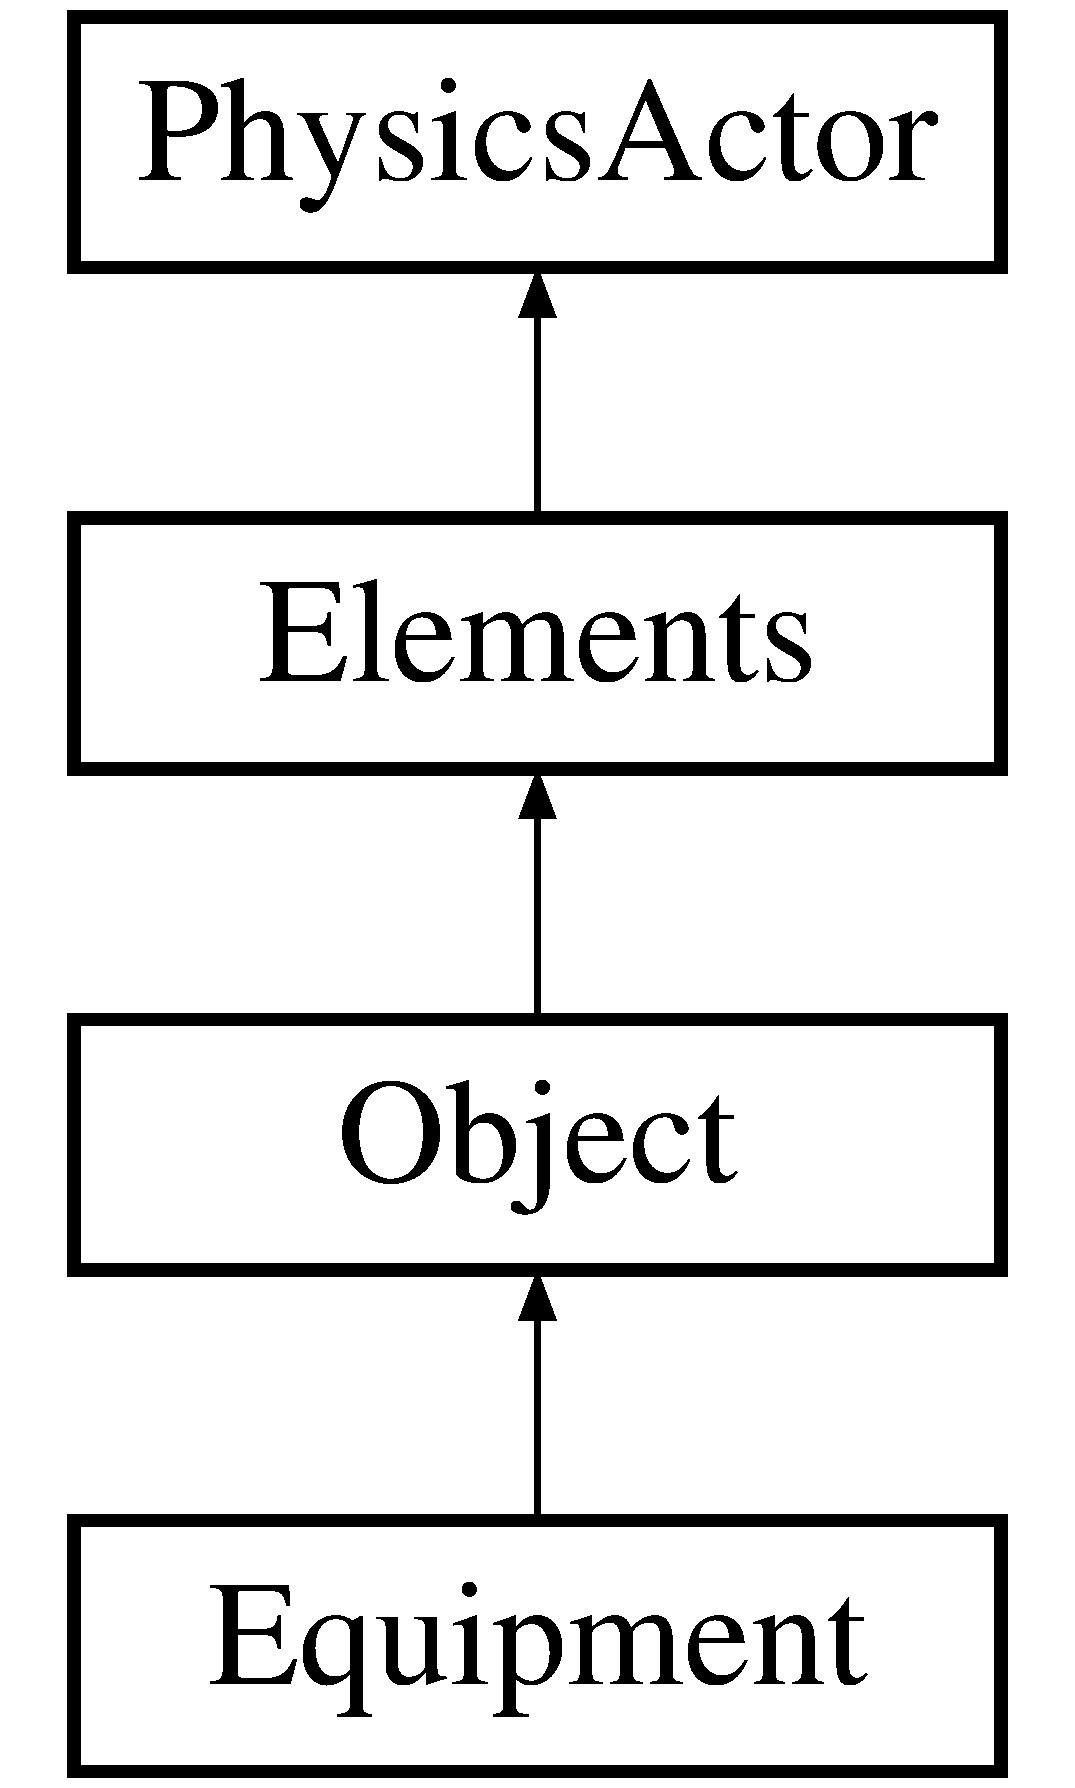
\includegraphics[height=4.000000cm]{class_equipment}
\end{center}
\end{figure}
\subsection*{Public Member Functions}
\begin{DoxyCompactItemize}
\item 
\hyperlink{class_equipment_a2bd67c4254f2074f4f7469f29a20e760}{Equipment} ()
\begin{DoxyCompactList}\small\item\em Basic constructor. \end{DoxyCompactList}\item 
\hyperlink{class_equipment_aeb2356275b65e0d7874aeaee05dc30a4}{Equipment} (\hyperlink{class_characters}{Characters} $\ast$)
\begin{DoxyCompactList}\small\item\em Constructor called when an enemy dies. \end{DoxyCompactList}\item 
\hypertarget{class_equipment_aad2bafad2e0b780e3451da80b5414a62}{{\bfseries Equipment} (\hyperlink{class_weapon}{Weapon} $\ast$, \hyperlink{class_characters}{Characters} $\ast$)}\label{class_equipment_aad2bafad2e0b780e3451da80b5414a62}

\item 
\hypertarget{class_equipment_a3e7f53e57fa3004b5a4490e2c7a1fbaf}{\hyperlink{class_equipment_a3e7f53e57fa3004b5a4490e2c7a1fbaf}{$\sim$\+Equipment} ()}\label{class_equipment_a3e7f53e57fa3004b5a4490e2c7a1fbaf}

\begin{DoxyCompactList}\small\item\em Destructor. \end{DoxyCompactList}\item 
\hypertarget{class_equipment_a54fd1c2d6cca6b4d2584eb0cf8725bd2}{\hyperlink{class_weapon}{Weapon} $\ast$ {\bfseries get\+Weapon} (void)}\label{class_equipment_a54fd1c2d6cca6b4d2584eb0cf8725bd2}

\item 
void \hyperlink{class_equipment_a0c706b45578e8d01fec7b8ee1b773987}{Begin\+Contact} (\hyperlink{class_elements}{Elements} $\ast$elem, b2\+Contact $\ast$contact)
\begin{DoxyCompactList}\small\item\em Collision begin callback. \end{DoxyCompactList}\item 
void \hyperlink{class_equipment_abda1acd976a1c33f3aa398b3a9a64555}{End\+Contact} (\hyperlink{class_elements}{Elements} $\ast$elem, b2\+Contact $\ast$contact)
\begin{DoxyCompactList}\small\item\em End of collision callback. \end{DoxyCompactList}\item 
void \hyperlink{class_equipment_ab195be955597ce6f64c117d675df3af4}{Receive\+Message} (Message $\ast$m)
\begin{DoxyCompactList}\small\item\em Intern broadcasts function. \end{DoxyCompactList}\end{DoxyCompactItemize}
\subsection*{Additional Inherited Members}


\subsection{Detailed Description}
Licensed to the Apache Software Foundation (A\+S\+F) under one or more contributor license agreements. See the N\+O\+T\+I\+C\+E file distributed with this work for additional information regarding copyright ownership. The A\+S\+F licenses this file to you under the Apache License, Version 2.\+0 (the \char`\"{}\+License\char`\"{}); you may not use this file except in compliance with the License. You may obtain a copy of the License at

\href{http://www.apache.org/licenses/LICENSE-2.0}{\tt http\+://www.\+apache.\+org/licenses/\+L\+I\+C\+E\+N\+S\+E-\/2.\+0}

Unless required by applicable law or agreed to in writing, software distributed under the License is distributed on an \char`\"{}\+A\+S I\+S\char`\"{} B\+A\+S\+I\+S, W\+I\+T\+H\+O\+U\+T W\+A\+R\+R\+A\+N\+T\+I\+E\+S O\+R C\+O\+N\+D\+I\+T\+I\+O\+N\+S O\+F A\+N\+Y K\+I\+N\+D, either express or implied. See the License for the specific language governing permissions and limitations under the License. File\+: \hyperlink{_equipment_8hpp_source}{Equipment.\+hpp} Creation\+: 2015-\/03-\/06 15\+:51 Manon Budin \href{mailto:mbudin@student.42.fr}{\tt mbudin@student.\+42.\+fr} 

\subsection{Constructor \& Destructor Documentation}
\hypertarget{class_equipment_a2bd67c4254f2074f4f7469f29a20e760}{\index{Equipment@{Equipment}!Equipment@{Equipment}}
\index{Equipment@{Equipment}!Equipment@{Equipment}}
\subsubsection[{Equipment}]{\setlength{\rightskip}{0pt plus 5cm}Equipment\+::\+Equipment (
\begin{DoxyParamCaption}
\item[{void}]{}
\end{DoxyParamCaption}
)}}\label{class_equipment_a2bd67c4254f2074f4f7469f29a20e760}


Basic constructor. 

Licensed to the Apache Software Foundation (A\+S\+F) under one or more contributor license agreements. See the N\+O\+T\+I\+C\+E file distributed with this work for additional information regarding copyright ownership. The A\+S\+F licenses this file to you under the Apache License, Version 2.\+0 (the \char`\"{}\+License\char`\"{}); you may not use this file except in compliance with the License. You may obtain a copy of the License at

\href{http://www.apache.org/licenses/LICENSE-2.0}{\tt http\+://www.\+apache.\+org/licenses/\+L\+I\+C\+E\+N\+S\+E-\/2.\+0}

Unless required by applicable law or agreed to in writing, software distributed under the License is distributed on an \char`\"{}\+A\+S I\+S\char`\"{} B\+A\+S\+I\+S, W\+I\+T\+H\+O\+U\+T W\+A\+R\+R\+A\+N\+T\+I\+E\+S O\+R C\+O\+N\+D\+I\+T\+I\+O\+N\+S O\+F A\+N\+Y K\+I\+N\+D, either express or implied. See the License for the specific language governing permissions and limitations under the License. File\+: Equipment.\+cpp Creation\+: 2015-\/03-\/06 15\+:51 Manon Budin \href{mailto:mbudin@student.42.fr}{\tt mbudin@student.\+42.\+fr} The basic constructor. In this constructor, we get the sprite and Init\+Physics. \begin{DoxyRefDesc}{Todo}
\item[\hyperlink{todo__todo000005}{Todo}]The position is actually in the hard-\/way. Config file needed. \end{DoxyRefDesc}
\hypertarget{class_equipment_aeb2356275b65e0d7874aeaee05dc30a4}{\index{Equipment@{Equipment}!Equipment@{Equipment}}
\index{Equipment@{Equipment}!Equipment@{Equipment}}
\subsubsection[{Equipment}]{\setlength{\rightskip}{0pt plus 5cm}Equipment\+::\+Equipment (
\begin{DoxyParamCaption}
\item[{{\bf Characters} $\ast$}]{c}
\end{DoxyParamCaption}
)}}\label{class_equipment_aeb2356275b65e0d7874aeaee05dc30a4}


Constructor called when an enemy dies. 

This constructor positions the object based on the enemy 
\begin{DoxyParams}{Parameters}
{\em c} & (A \hyperlink{class_characters}{Characters} object) \\
\hline
\end{DoxyParams}


\subsection{Member Function Documentation}
\hypertarget{class_equipment_a0c706b45578e8d01fec7b8ee1b773987}{\index{Equipment@{Equipment}!Begin\+Contact@{Begin\+Contact}}
\index{Begin\+Contact@{Begin\+Contact}!Equipment@{Equipment}}
\subsubsection[{Begin\+Contact}]{\setlength{\rightskip}{0pt plus 5cm}void Equipment\+::\+Begin\+Contact (
\begin{DoxyParamCaption}
\item[{{\bf Elements} $\ast$}]{elem, }
\item[{b2\+Contact $\ast$}]{contact}
\end{DoxyParamCaption}
)\hspace{0.3cm}{\ttfamily [virtual]}}}\label{class_equipment_a0c706b45578e8d01fec7b8ee1b773987}


Collision begin callback. 

The contact begin function /!\textbackslash{} This function is actually called just B\+E\+F\+O\+R\+E a collision 
\begin{DoxyParams}{Parameters}
{\em elem} & The \hyperlink{class_elements}{Elements} who collide with. \\
\hline
{\em contact} & The Box2\+D contact object. \\
\hline
\end{DoxyParams}


Reimplemented from \hyperlink{class_elements}{Elements}.

\hypertarget{class_equipment_abda1acd976a1c33f3aa398b3a9a64555}{\index{Equipment@{Equipment}!End\+Contact@{End\+Contact}}
\index{End\+Contact@{End\+Contact}!Equipment@{Equipment}}
\subsubsection[{End\+Contact}]{\setlength{\rightskip}{0pt plus 5cm}void Equipment\+::\+End\+Contact (
\begin{DoxyParamCaption}
\item[{{\bf Elements} $\ast$}]{elem, }
\item[{b2\+Contact $\ast$}]{contact}
\end{DoxyParamCaption}
)\hspace{0.3cm}{\ttfamily [virtual]}}}\label{class_equipment_abda1acd976a1c33f3aa398b3a9a64555}


End of collision callback. 

End of contact function /!\textbackslash{} This function is called just after the collision is over, 
\begin{DoxyParams}{Parameters}
{\em elem} & The other element \\
\hline
{\em contact} & The Box2\+D contact object \\
\hline
\end{DoxyParams}


Reimplemented from \hyperlink{class_elements}{Elements}.

\hypertarget{class_equipment_ab195be955597ce6f64c117d675df3af4}{\index{Equipment@{Equipment}!Receive\+Message@{Receive\+Message}}
\index{Receive\+Message@{Receive\+Message}!Equipment@{Equipment}}
\subsubsection[{Receive\+Message}]{\setlength{\rightskip}{0pt plus 5cm}void Equipment\+::\+Receive\+Message (
\begin{DoxyParamCaption}
\item[{Message $\ast$}]{m}
\end{DoxyParamCaption}
)}}\label{class_equipment_ab195be955597ce6f64c117d675df3af4}


Intern broadcasts function. 

The Receive Message function. 
\begin{DoxyParams}{Parameters}
{\em m} & The Broadcasted message. (See Angel2\+D docs for more info.) \\
\hline
\end{DoxyParams}


The documentation for this class was generated from the following files\+:\begin{DoxyCompactItemize}
\item 
inc/Equipment.\+hpp\item 
src/Equipment.\+cpp\end{DoxyCompactItemize}

\hypertarget{class_game}{\section{Game Class Reference}
\label{class_game}\index{Game@{Game}}
}
\subsection*{Public Member Functions}
\begin{DoxyCompactItemize}
\item 
\hyperlink{class_game_ad59df6562a58a614fda24622d3715b65}{Game} ()
\begin{DoxyCompactList}\small\item\em Basic constructor, set the window to default value. \end{DoxyCompactList}\item 
\hyperlink{class_game_a20220a5fdc31f41d6c642f70204799d0}{Game} (unsigned int width, unsigned int height)
\item 
\hyperlink{class_game_ae3d112ca6e0e55150d2fdbc704474530}{$\sim$\+Game} ()
\item 
void \hyperlink{class_game_a616466e4850732139841c148ed18c05f}{grid} (void)
\item 
void \hyperlink{class_game_a662a1969275a12a8ffebf2e53e8c843a}{start} (void)
\item 
void \hyperlink{class_game_af06f40bacd46f8facba328648cb221b5}{read\+Maps} (void)
\begin{DoxyCompactList}\small\item\em Read the maps. \end{DoxyCompactList}\item 
void \hyperlink{class_game_a82b79f027868bb70c2325f473a0270a9}{display\+Hero} (\hyperlink{class_elements}{Elements} \&\hyperlink{class_hero}{Hero})
\begin{DoxyCompactList}\small\item\em Display the \hyperlink{class_hero}{Hero}. \end{DoxyCompactList}\item 
void \hyperlink{class_game_abbb01372bc9b6703a49d5960fb62ff0b}{display\+Enemy} (\hyperlink{class_elements}{Elements} \&\hyperlink{class_enemy}{Enemy})
\begin{DoxyCompactList}\small\item\em Display the \hyperlink{class_enemy}{Enemy}. \end{DoxyCompactList}\item 
void \hyperlink{class_game_a6ce6fb87e236965d8b1d3ca7143337f6}{display\+Object} (\hyperlink{class_elements}{Elements} \&\hyperlink{class_object}{Object})
\begin{DoxyCompactList}\small\item\em Display the object. \end{DoxyCompactList}\item 
void \hyperlink{class_game_ab1ab415f40c6a952da0f93a7bf3ffee1}{show\+Map} (void)
\begin{DoxyCompactList}\small\item\em Display the first map. \end{DoxyCompactList}\item 
void \hyperlink{class_game_a194dbc017575c98bda4e2317d266a67e}{display\+H\+U\+D} (void)
\begin{DoxyCompactList}\small\item\em Display the base H\+U\+D. \end{DoxyCompactList}\item 
\hypertarget{class_game_a730c7eeaa90f5ceab71abce303bfd367}{void {\bfseries set\+Hero} (\hyperlink{class_characters}{Characters} \&h)}\label{class_game_a730c7eeaa90f5ceab71abce303bfd367}

\item 
\hypertarget{class_game_a7f62e55c834c5ee4b626acb58f5bbd28}{\hyperlink{class_characters}{Characters} \& {\bfseries get\+Hero} (void)}\label{class_game_a7f62e55c834c5ee4b626acb58f5bbd28}

\end{DoxyCompactItemize}
\subsection*{Static Public Member Functions}
\begin{DoxyCompactItemize}
\item 
static void \hyperlink{class_game_ae391a35eb1f970669b0d6b236de4b885}{destroy\+All\+Bodies} (void)
\begin{DoxyCompactList}\small\item\em Intern callback for destroying an element. \end{DoxyCompactList}\item 
static void \hyperlink{class_game_ae3c5dc329506d37d244ef3587ac813af}{add\+To\+Destroy\+List} (\hyperlink{class_elements}{Elements} $\ast$m)
\begin{DoxyCompactList}\small\item\em Destroy an element at the right time. \end{DoxyCompactList}\item 
static int \hyperlink{class_game_aec4cafc10218eb665d67bf027ddbd3f1}{get\+Next\+Id} (void)
\begin{DoxyCompactList}\small\item\em Get an id, in order. \end{DoxyCompactList}\item 
static void \hyperlink{class_game_a10d84bf0157d5b3abf102846d5170af5}{add\+Element} (\hyperlink{class_elements}{Elements} \&elem)
\begin{DoxyCompactList}\small\item\em Add an Element. \end{DoxyCompactList}\item 
static void \hyperlink{class_game_a644e15f76310ed410817e8423ad7a5b2}{del\+Element} (\hyperlink{class_elements}{Elements} $\ast$elem)
\begin{DoxyCompactList}\small\item\em Delete an element. \end{DoxyCompactList}\item 
\hypertarget{class_game_aafc84f0b25d07825f08dffc07af73918}{static void {\bfseries list\+Element} (void)}\label{class_game_aafc84f0b25d07825f08dffc07af73918}

\item 
static void \hyperlink{class_game_a34c8791251f785d270f757b6eff4ea56}{call\+Callbacks} (int a, int b)
\begin{DoxyCompactList}\small\item\em Collision intern callbacks. \end{DoxyCompactList}\item 
static void \hyperlink{class_game_a27ad8f2a6f8f098cc28377df13c4ec2e}{start\+Running} (\hyperlink{class_elements}{Elements} $\ast$c)
\begin{DoxyCompactList}\small\item\em Intern callback for staring running. \end{DoxyCompactList}\item 
static void \hyperlink{class_game_a9394f6f0c90bde35fb0bd4ca3316c3f0}{stop\+Running} (\hyperlink{class_elements}{Elements} $\ast$c)
\begin{DoxyCompactList}\small\item\em Intern callback for stoping running. \end{DoxyCompactList}\item 
static void \hyperlink{class_game_ae763ecd953645a586b638a46b908ca5a}{make\+It\+Run} (void)
\begin{DoxyCompactList}\small\item\em World Callback for making elements running. \end{DoxyCompactList}\item 
static void \hyperlink{class_game_a5cf54b4cf9d8bf024f8936fedf11ccea}{show\+Text} (void)
\begin{DoxyCompactList}\small\item\em Intern callback for display text. \end{DoxyCompactList}\item 
static void \hyperlink{class_game_a88d713d54d9303c38c897635c7c04cf4}{add\+H\+U\+D\+Window} (\hyperlink{class_h_u_d_window}{H\+U\+D\+Window} $\ast$)
\begin{DoxyCompactList}\small\item\em Register an H\+U\+D to the \hyperlink{class_game}{Game} list. \end{DoxyCompactList}\item 
static void \hyperlink{class_game_a80e17eab80071411eff5eb38d6b7fc76}{remove\+H\+U\+D\+Window} (\hyperlink{class_h_u_d_window}{H\+U\+D\+Window} $\ast$)
\begin{DoxyCompactList}\small\item\em Unregister an H\+U\+D to the \hyperlink{class_game}{Game} list. \end{DoxyCompactList}\item 
static \hyperlink{class_h_u_d_window}{H\+U\+D\+Window} $\ast$ \hyperlink{class_game_a8339342d69fc241d349da9404ce088c5}{get\+H\+U\+D} (void)
\begin{DoxyCompactList}\small\item\em Get the first / main H\+U\+D. \end{DoxyCompactList}\end{DoxyCompactItemize}
\subsection*{Public Attributes}
\begin{DoxyCompactItemize}
\item 
\hypertarget{class_game_adef62d41374c1440a78855c7f9994697}{\hyperlink{class_maps}{Maps} $\ast$ {\bfseries maps}}\label{class_game_adef62d41374c1440a78855c7f9994697}

\end{DoxyCompactItemize}
\subsection*{Static Public Attributes}
\begin{DoxyCompactItemize}
\item 
\hypertarget{class_game_a6f05b1c88b1086147854b72defced72a}{static bool {\bfseries end\+Game} = false}\label{class_game_a6f05b1c88b1086147854b72defced72a}

\item 
\hypertarget{class_game_aa7b98d72784b65dbef9070b638542b05}{static bool {\bfseries ended} = false}\label{class_game_aa7b98d72784b65dbef9070b638542b05}

\item 
\hypertarget{class_game_ac52883575849c7580b0b9dba48aef174}{static int {\bfseries lol}}\label{class_game_ac52883575849c7580b0b9dba48aef174}

\item 
\hypertarget{class_game_ae5bfa29230411c2605787261070909e6}{static int {\bfseries current\+Ids} = 0}\label{class_game_ae5bfa29230411c2605787261070909e6}

\item 
\hypertarget{class_game_a88aa459a01bbc438e665a19c53732c0e}{static std\+::map$<$ int, \hyperlink{class_elements}{Elements} $\ast$ $>$ {\bfseries element\+Map} = \{\}}\label{class_game_a88aa459a01bbc438e665a19c53732c0e}

\item 
\hypertarget{class_game_a078c48086258daf73a89bf4bde485969}{static std\+::list$<$ \hyperlink{class_elements}{Elements} $\ast$ $>$ {\bfseries bodies\+To\+Destroy}}\label{class_game_a078c48086258daf73a89bf4bde485969}

\item 
\hypertarget{class_game_a04166a78d83b34000f7ab31d867fef27}{static std\+::list$<$ \hyperlink{class_elements}{Elements} $\ast$ $>$ {\bfseries bodies\+To\+Create}}\label{class_game_a04166a78d83b34000f7ab31d867fef27}

\item 
\hypertarget{class_game_a80912de3bec452b5a8df21650422d20a}{static std\+::list$<$ \hyperlink{class_elements}{Elements} $\ast$ $>$ {\bfseries running\+Charac}}\label{class_game_a80912de3bec452b5a8df21650422d20a}

\item 
\hypertarget{class_game_afa3edaf9ec297d522ea19cd48c77a53a}{static std\+::list$<$ \hyperlink{class_h_u_d_window}{H\+U\+D\+Window} $\ast$ $>$ {\bfseries windows}}\label{class_game_afa3edaf9ec297d522ea19cd48c77a53a}

\item 
\hypertarget{class_game_afa1de8c59db49bc9239f6bb87465351b}{static \hyperlink{class_weapon_list}{Weapon\+List} $\ast$ {\bfseries w\+List}}\label{class_game_afa1de8c59db49bc9239f6bb87465351b}

\item 
\hypertarget{class_game_a5625cb138092a97f084bd65c0e0af173}{static \hyperlink{class_hitbox}{Hitbox} $\ast$ {\bfseries h\+List}}\label{class_game_a5625cb138092a97f084bd65c0e0af173}

\end{DoxyCompactItemize}


\subsection{Constructor \& Destructor Documentation}
\hypertarget{class_game_ad59df6562a58a614fda24622d3715b65}{\index{Game@{Game}!Game@{Game}}
\index{Game@{Game}!Game@{Game}}
\subsubsection[{Game}]{\setlength{\rightskip}{0pt plus 5cm}Game\+::\+Game (
\begin{DoxyParamCaption}
\item[{void}]{}
\end{DoxyParamCaption}
)}}\label{class_game_ad59df6562a58a614fda24622d3715b65}


Basic constructor, set the window to default value. 

Licensed to the Apache Software Foundation (A\+S\+F) under one or more contributor license agreements. See the N\+O\+T\+I\+C\+E file distributed with this work for additional information regarding copyright ownership. The A\+S\+F licenses this file to you under the Apache License, Version 2.\+0 (the \char`\"{}\+License\char`\"{}); you may not use this file except in compliance with the License. You may obtain a copy of the License at

\href{http://www.apache.org/licenses/LICENSE-2.0}{\tt http\+://www.\+apache.\+org/licenses/\+L\+I\+C\+E\+N\+S\+E-\/2.\+0}

Unless required by applicable law or agreed to in writing, software distributed under the License is distributed on an \char`\"{}\+A\+S I\+S\char`\"{} B\+A\+S\+I\+S, W\+I\+T\+H\+O\+U\+T W\+A\+R\+R\+A\+N\+T\+I\+E\+S O\+R C\+O\+N\+D\+I\+T\+I\+O\+N\+S O\+F A\+N\+Y K\+I\+N\+D, either express or implied. See the License for the specific language governing permissions and limitations under the License. File\+: Game.\+cpp \begin{DoxyDate}{Date}
2015-\/02-\/13 07\+:20 
\end{DoxyDate}
\begin{DoxyAuthor}{Author}
Louis Solofrizzo \href{mailto:louis@ne02ptzero.me}{\tt louis@ne02ptzero.\+me} Initialize the world window, init Physics. (\href{http://docs.angel2d.com/class_world.html#ae5d7e8d20d3e6fc93785ab2014ac0c13}{\tt http\+://docs.\+angel2d.\+com/class\+\_\+world.\+html\#ae5d7e8d20d3e6fc93785ab2014ac0c13}) Load the maps with \hyperlink{class_maps_a87e73431397d1c36dcc2a95ef2b00732}{Maps\+::\+Maps} 
\end{DoxyAuthor}
\begin{DoxySeeAlso}{See also}
\hyperlink{class_maps}{Maps} 
\end{DoxySeeAlso}
\hypertarget{class_game_a20220a5fdc31f41d6c642f70204799d0}{\index{Game@{Game}!Game@{Game}}
\index{Game@{Game}!Game@{Game}}
\subsubsection[{Game}]{\setlength{\rightskip}{0pt plus 5cm}Game\+::\+Game (
\begin{DoxyParamCaption}
\item[{unsigned int}]{width, }
\item[{unsigned int}]{height}
\end{DoxyParamCaption}
)}}\label{class_game_a20220a5fdc31f41d6c642f70204799d0}
Constructor with custom window width \& height 
\begin{DoxyParams}{Parameters}
{\em width} & The width of the window \\
\hline
{\em heigh} & The height of the window \\
\hline
\end{DoxyParams}
\hypertarget{class_game_ae3d112ca6e0e55150d2fdbc704474530}{\index{Game@{Game}!````~Game@{$\sim$\+Game}}
\index{````~Game@{$\sim$\+Game}!Game@{Game}}
\subsubsection[{$\sim$\+Game}]{\setlength{\rightskip}{0pt plus 5cm}Game\+::$\sim$\+Game (
\begin{DoxyParamCaption}
\item[{void}]{}
\end{DoxyParamCaption}
)}}\label{class_game_ae3d112ca6e0e55150d2fdbc704474530}
Destructor 

\subsection{Member Function Documentation}
\hypertarget{class_game_a10d84bf0157d5b3abf102846d5170af5}{\index{Game@{Game}!add\+Element@{add\+Element}}
\index{add\+Element@{add\+Element}!Game@{Game}}
\subsubsection[{add\+Element}]{\setlength{\rightskip}{0pt plus 5cm}void Game\+::add\+Element (
\begin{DoxyParamCaption}
\item[{{\bf Elements} \&}]{elem}
\end{DoxyParamCaption}
)\hspace{0.3cm}{\ttfamily [static]}}}\label{class_game_a10d84bf0157d5b3abf102846d5170af5}


Add an Element. 

Add an element to the intern map, to the static elements map. This map is usefull for cleaning an all level, or fading out at death, etc. 
\begin{DoxyParams}{Parameters}
{\em elem} & The \hyperlink{class_elements}{Elements} to add at the list \\
\hline
\end{DoxyParams}
\hypertarget{class_game_a88d713d54d9303c38c897635c7c04cf4}{\index{Game@{Game}!add\+H\+U\+D\+Window@{add\+H\+U\+D\+Window}}
\index{add\+H\+U\+D\+Window@{add\+H\+U\+D\+Window}!Game@{Game}}
\subsubsection[{add\+H\+U\+D\+Window}]{\setlength{\rightskip}{0pt plus 5cm}void Game\+::add\+H\+U\+D\+Window (
\begin{DoxyParamCaption}
\item[{{\bf H\+U\+D\+Window} $\ast$}]{w}
\end{DoxyParamCaption}
)\hspace{0.3cm}{\ttfamily [static]}}}\label{class_game_a88d713d54d9303c38c897635c7c04cf4}


Register an H\+U\+D to the \hyperlink{class_game}{Game} list. 

Add a \hyperlink{class_h_u_d_window}{H\+U\+D\+Window} object to the callback list. 
\begin{DoxyParams}{Parameters}
{\em w} & The new H\+U\+D to add in \hyperlink{class_game}{Game}. \\
\hline
\end{DoxyParams}
\hypertarget{class_game_ae3c5dc329506d37d244ef3587ac813af}{\index{Game@{Game}!add\+To\+Destroy\+List@{add\+To\+Destroy\+List}}
\index{add\+To\+Destroy\+List@{add\+To\+Destroy\+List}!Game@{Game}}
\subsubsection[{add\+To\+Destroy\+List}]{\setlength{\rightskip}{0pt plus 5cm}void Game\+::add\+To\+Destroy\+List (
\begin{DoxyParamCaption}
\item[{{\bf Elements} $\ast$}]{m}
\end{DoxyParamCaption}
)\hspace{0.3cm}{\ttfamily [static]}}}\label{class_game_ae3c5dc329506d37d244ef3587ac813af}


Destroy an element at the right time. 

Call to add an element to the destroy list after the tick() This function D\+O N\+O\+T remove an element itself. We stock in a list, and after the World\+::tick, we call a function to destroying each element of the list. 
\begin{DoxyParams}{Parameters}
{\em m} & The Element to destroy \\
\hline
\end{DoxyParams}
\begin{DoxyRefDesc}{Todo}
\item[\hyperlink{todo__todo000006}{Todo}]how the fuck does String\+Set works? Needed here for the Unsubscribe\+From\+All \end{DoxyRefDesc}
\hypertarget{class_game_a34c8791251f785d270f757b6eff4ea56}{\index{Game@{Game}!call\+Callbacks@{call\+Callbacks}}
\index{call\+Callbacks@{call\+Callbacks}!Game@{Game}}
\subsubsection[{call\+Callbacks}]{\setlength{\rightskip}{0pt plus 5cm}void Game\+::call\+Callbacks (
\begin{DoxyParamCaption}
\item[{int}]{a, }
\item[{int}]{b}
\end{DoxyParamCaption}
)\hspace{0.3cm}{\ttfamily [static]}}}\label{class_game_a34c8791251f785d270f757b6eff4ea56}


Collision intern callbacks. 

Call the collision callbacks on two objects 
\begin{DoxyParams}{Parameters}
{\em a} & The I\+D of the first object \\
\hline
{\em b} & The I\+D of the second object \\
\hline
\end{DoxyParams}
\hypertarget{class_game_a644e15f76310ed410817e8423ad7a5b2}{\index{Game@{Game}!del\+Element@{del\+Element}}
\index{del\+Element@{del\+Element}!Game@{Game}}
\subsubsection[{del\+Element}]{\setlength{\rightskip}{0pt plus 5cm}void Game\+::del\+Element (
\begin{DoxyParamCaption}
\item[{{\bf Elements} $\ast$}]{elem}
\end{DoxyParamCaption}
)\hspace{0.3cm}{\ttfamily [static]}}}\label{class_game_a644e15f76310ed410817e8423ad7a5b2}


Delete an element. 

Delete an element from the intern map 
\begin{DoxyParams}{Parameters}
{\em elem} & The element to delete (The reference is important !) \\
\hline
\end{DoxyParams}
\hypertarget{class_game_ae391a35eb1f970669b0d6b236de4b885}{\index{Game@{Game}!destroy\+All\+Bodies@{destroy\+All\+Bodies}}
\index{destroy\+All\+Bodies@{destroy\+All\+Bodies}!Game@{Game}}
\subsubsection[{destroy\+All\+Bodies}]{\setlength{\rightskip}{0pt plus 5cm}void Game\+::destroy\+All\+Bodies (
\begin{DoxyParamCaption}
\item[{void}]{}
\end{DoxyParamCaption}
)\hspace{0.3cm}{\ttfamily [static]}}}\label{class_game_ae391a35eb1f970669b0d6b236de4b885}


Intern callback for destroying an element. 

Called after each tick() in order to destroy all elements set to destroy. This function destroy each element in Game\+::bodies\+To\+Destroy. So, call this function outisde of this goal is useless. \hypertarget{class_game_abbb01372bc9b6703a49d5960fb62ff0b}{\index{Game@{Game}!display\+Enemy@{display\+Enemy}}
\index{display\+Enemy@{display\+Enemy}!Game@{Game}}
\subsubsection[{display\+Enemy}]{\setlength{\rightskip}{0pt plus 5cm}void Game\+::display\+Enemy (
\begin{DoxyParamCaption}
\item[{{\bf Elements} \&}]{Enemy}
\end{DoxyParamCaption}
)}}\label{class_game_abbb01372bc9b6703a49d5960fb62ff0b}


Display the \hyperlink{class_enemy}{Enemy}. 

Add an \hyperlink{class_enemy}{Enemy} to the world, with an init position (x, y) 
\begin{DoxyParams}{Parameters}
{\em \hyperlink{class_enemy}{Enemy}} & The enemy object \\
\hline
\end{DoxyParams}
\hypertarget{class_game_a82b79f027868bb70c2325f473a0270a9}{\index{Game@{Game}!display\+Hero@{display\+Hero}}
\index{display\+Hero@{display\+Hero}!Game@{Game}}
\subsubsection[{display\+Hero}]{\setlength{\rightskip}{0pt plus 5cm}void Game\+::display\+Hero (
\begin{DoxyParamCaption}
\item[{{\bf Elements} \&}]{Hero}
\end{DoxyParamCaption}
)}}\label{class_game_a82b79f027868bb70c2325f473a0270a9}


Display the \hyperlink{class_hero}{Hero}. 

We add the hero to the world, with an init position (x, y) 
\begin{DoxyParams}{Parameters}
{\em \hyperlink{class_hero}{Hero}} & The \hyperlink{class_hero}{Hero} \hyperlink{class_object}{Object} \\
\hline
\end{DoxyParams}
\hypertarget{class_game_a194dbc017575c98bda4e2317d266a67e}{\index{Game@{Game}!display\+H\+U\+D@{display\+H\+U\+D}}
\index{display\+H\+U\+D@{display\+H\+U\+D}!Game@{Game}}
\subsubsection[{display\+H\+U\+D}]{\setlength{\rightskip}{0pt plus 5cm}void Game\+::display\+H\+U\+D (
\begin{DoxyParamCaption}
\item[{void}]{}
\end{DoxyParamCaption}
)}}\label{class_game_a194dbc017575c98bda4e2317d266a67e}


Display the base H\+U\+D. 

The init function for display the base H\+U\+D. \begin{DoxyRefDesc}{Todo}
\item[\hyperlink{todo__todo000007}{Todo}]This function is nasty, we need a recap here. \end{DoxyRefDesc}
\hypertarget{class_game_a6ce6fb87e236965d8b1d3ca7143337f6}{\index{Game@{Game}!display\+Object@{display\+Object}}
\index{display\+Object@{display\+Object}!Game@{Game}}
\subsubsection[{display\+Object}]{\setlength{\rightskip}{0pt plus 5cm}void Game\+::display\+Object (
\begin{DoxyParamCaption}
\item[{{\bf Elements} \&}]{Object}
\end{DoxyParamCaption}
)}}\label{class_game_a6ce6fb87e236965d8b1d3ca7143337f6}


Display the object. 

Display the \hyperlink{class_object}{Object} ?!  Does this function have a real utility now ? 
\begin{DoxyParams}{Parameters}
{\em \hyperlink{class_object}{Object}} & The \hyperlink{class_object}{Object} \\
\hline
\end{DoxyParams}
\hypertarget{class_game_a8339342d69fc241d349da9404ce088c5}{\index{Game@{Game}!get\+H\+U\+D@{get\+H\+U\+D}}
\index{get\+H\+U\+D@{get\+H\+U\+D}!Game@{Game}}
\subsubsection[{get\+H\+U\+D}]{\setlength{\rightskip}{0pt plus 5cm}{\bf H\+U\+D\+Window} $\ast$ Game\+::get\+H\+U\+D (
\begin{DoxyParamCaption}
\item[{void}]{}
\end{DoxyParamCaption}
)\hspace{0.3cm}{\ttfamily [static]}}}\label{class_game_a8339342d69fc241d349da9404ce088c5}


Get the first / main H\+U\+D. 

Get the first H\+U\+D from the list. (Assuming there is an element) This function is generaly use for getting the main H\+U\+D (life, xp, items) object, assuming this object is the first added to the list. \hypertarget{class_game_aec4cafc10218eb665d67bf027ddbd3f1}{\index{Game@{Game}!get\+Next\+Id@{get\+Next\+Id}}
\index{get\+Next\+Id@{get\+Next\+Id}!Game@{Game}}
\subsubsection[{get\+Next\+Id}]{\setlength{\rightskip}{0pt plus 5cm}int Game\+::get\+Next\+Id (
\begin{DoxyParamCaption}
\item[{void}]{}
\end{DoxyParamCaption}
)\hspace{0.3cm}{\ttfamily [static]}}}\label{class_game_aec4cafc10218eb665d67bf027ddbd3f1}


Get an id, in order. 

Get the current id, for the intern elements map \begin{DoxyReturn}{Returns}
The next id 
\end{DoxyReturn}
\hypertarget{class_game_a616466e4850732139841c148ed18c05f}{\index{Game@{Game}!grid@{grid}}
\index{grid@{grid}!Game@{Game}}
\subsubsection[{grid}]{\setlength{\rightskip}{0pt plus 5cm}void Game\+::grid (
\begin{DoxyParamCaption}
\item[{void}]{}
\end{DoxyParamCaption}
)}}\label{class_game_a616466e4850732139841c148ed18c05f}
Add a grid to the world (D\+E\+B\+U\+G) \hypertarget{class_game_ae763ecd953645a586b638a46b908ca5a}{\index{Game@{Game}!make\+It\+Run@{make\+It\+Run}}
\index{make\+It\+Run@{make\+It\+Run}!Game@{Game}}
\subsubsection[{make\+It\+Run}]{\setlength{\rightskip}{0pt plus 5cm}void Game\+::make\+It\+Run (
\begin{DoxyParamCaption}
\item[{void}]{}
\end{DoxyParamCaption}
)\hspace{0.3cm}{\ttfamily [static]}}}\label{class_game_ae763ecd953645a586b638a46b908ca5a}


World Callback for making elements running. 

The callback for each frame, making the call to the interns callbacks. This function call the function \+\_\+run for each member of the list Game\+::running\+Charac Keep this in mind, you won't probably call this function. \begin{DoxySeeAlso}{See also}
\hyperlink{class_characters}{Characters} 
\end{DoxySeeAlso}
\hypertarget{class_game_af06f40bacd46f8facba328648cb221b5}{\index{Game@{Game}!read\+Maps@{read\+Maps}}
\index{read\+Maps@{read\+Maps}!Game@{Game}}
\subsubsection[{read\+Maps}]{\setlength{\rightskip}{0pt plus 5cm}void Game\+::read\+Maps (
\begin{DoxyParamCaption}
\item[{void}]{}
\end{DoxyParamCaption}
)}}\label{class_game_af06f40bacd46f8facba328648cb221b5}


Read the maps. 

Launch \hyperlink{class_maps_a65ebe26294d69e741ee94d5530597886}{Maps\+::read\+Maps} \begin{DoxySeeAlso}{See also}
\hyperlink{class_maps}{Maps} 
\end{DoxySeeAlso}
\hypertarget{class_game_a80e17eab80071411eff5eb38d6b7fc76}{\index{Game@{Game}!remove\+H\+U\+D\+Window@{remove\+H\+U\+D\+Window}}
\index{remove\+H\+U\+D\+Window@{remove\+H\+U\+D\+Window}!Game@{Game}}
\subsubsection[{remove\+H\+U\+D\+Window}]{\setlength{\rightskip}{0pt plus 5cm}void Game\+::remove\+H\+U\+D\+Window (
\begin{DoxyParamCaption}
\item[{{\bf H\+U\+D\+Window} $\ast$}]{w}
\end{DoxyParamCaption}
)\hspace{0.3cm}{\ttfamily [static]}}}\label{class_game_a80e17eab80071411eff5eb38d6b7fc76}


Unregister an H\+U\+D to the \hyperlink{class_game}{Game} list. 

Remove a \hyperlink{class_h_u_d_window}{H\+U\+D\+Window} from the callback list. 
\begin{DoxyParams}{Parameters}
{\em w} & The \hyperlink{class_h_u_d_window}{H\+U\+D\+Window} to delete. \\
\hline
\end{DoxyParams}
\hypertarget{class_game_ab1ab415f40c6a952da0f93a7bf3ffee1}{\index{Game@{Game}!show\+Map@{show\+Map}}
\index{show\+Map@{show\+Map}!Game@{Game}}
\subsubsection[{show\+Map}]{\setlength{\rightskip}{0pt plus 5cm}void Game\+::show\+Map (
\begin{DoxyParamCaption}
\item[{void}]{}
\end{DoxyParamCaption}
)}}\label{class_game_ab1ab415f40c6a952da0f93a7bf3ffee1}


Display the first map. 

Call the function \hyperlink{class_maps_acc65a2a83bdad1c467531b3e25188b91}{Maps\+::first\+One} \begin{DoxySeeAlso}{See also}
\hyperlink{class_maps}{Maps} 
\end{DoxySeeAlso}
\hypertarget{class_game_a5cf54b4cf9d8bf024f8936fedf11ccea}{\index{Game@{Game}!show\+Text@{show\+Text}}
\index{show\+Text@{show\+Text}!Game@{Game}}
\subsubsection[{show\+Text}]{\setlength{\rightskip}{0pt plus 5cm}void Game\+::show\+Text (
\begin{DoxyParamCaption}
\item[{void}]{}
\end{DoxyParamCaption}
)\hspace{0.3cm}{\ttfamily [static]}}}\label{class_game_a5cf54b4cf9d8bf024f8936fedf11ccea}


Intern callback for display text. 

Callback for each frame, to display the text in the H\+U\+Ds. This function is just call the function display\+Text() on each member of the H\+U\+D\+List. Keep this in mind, you won't probably call this function. \hypertarget{class_game_a662a1969275a12a8ffebf2e53e8c843a}{\index{Game@{Game}!start@{start}}
\index{start@{start}!Game@{Game}}
\subsubsection[{start}]{\setlength{\rightskip}{0pt plus 5cm}void Game\+::start (
\begin{DoxyParamCaption}
\item[{void}]{}
\end{DoxyParamCaption}
)}}\label{class_game_a662a1969275a12a8ffebf2e53e8c843a}
Let's start the game \hypertarget{class_game_a27ad8f2a6f8f098cc28377df13c4ec2e}{\index{Game@{Game}!start\+Running@{start\+Running}}
\index{start\+Running@{start\+Running}!Game@{Game}}
\subsubsection[{start\+Running}]{\setlength{\rightskip}{0pt plus 5cm}void Game\+::start\+Running (
\begin{DoxyParamCaption}
\item[{{\bf Elements} $\ast$}]{c}
\end{DoxyParamCaption}
)\hspace{0.3cm}{\ttfamily [static]}}}\label{class_game_a27ad8f2a6f8f098cc28377df13c4ec2e}


Intern callback for staring running. 

Make an element running This function do not make the element 'running', just add them to the callback list. 
\begin{DoxyParams}{Parameters}
{\em c} & The Element who start running. \\
\hline
\end{DoxyParams}
\hypertarget{class_game_a9394f6f0c90bde35fb0bd4ca3316c3f0}{\index{Game@{Game}!stop\+Running@{stop\+Running}}
\index{stop\+Running@{stop\+Running}!Game@{Game}}
\subsubsection[{stop\+Running}]{\setlength{\rightskip}{0pt plus 5cm}void Game\+::stop\+Running (
\begin{DoxyParamCaption}
\item[{{\bf Elements} $\ast$}]{c}
\end{DoxyParamCaption}
)\hspace{0.3cm}{\ttfamily [static]}}}\label{class_game_a9394f6f0c90bde35fb0bd4ca3316c3f0}


Intern callback for stoping running. 

Make an element stop running. Same as \hyperlink{class_game_a27ad8f2a6f8f098cc28377df13c4ec2e}{Game\+::start\+Running()}, but the object is remove from the list. 
\begin{DoxyParams}{Parameters}
{\em c} & The \hyperlink{class_elements}{Elements} who stop running. \\
\hline
\end{DoxyParams}


The documentation for this class was generated from the following files\+:\begin{DoxyCompactItemize}
\item 
inc/Game.\+hpp\item 
src/Game.\+cpp\end{DoxyCompactItemize}

\hypertarget{class_game_contact_listener}{\section{Game\-Contact\-Listener Class Reference}
\label{class_game_contact_listener}\index{Game\-Contact\-Listener@{Game\-Contact\-Listener}}
}


{\ttfamily \#include $<$Game\-Contact\-Listener.\-hpp$>$}



Inheritance diagram for Game\-Contact\-Listener\-:\nopagebreak
\begin{figure}[H]
\begin{center}
\leavevmode
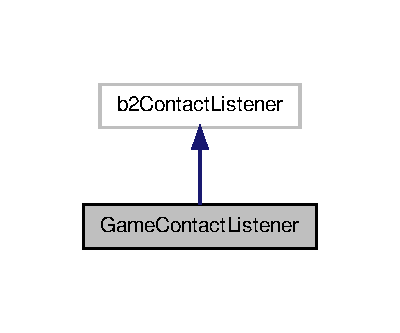
\includegraphics[width=192pt]{class_game_contact_listener__inherit__graph}
\end{center}
\end{figure}


Collaboration diagram for Game\-Contact\-Listener\-:\nopagebreak
\begin{figure}[H]
\begin{center}
\leavevmode
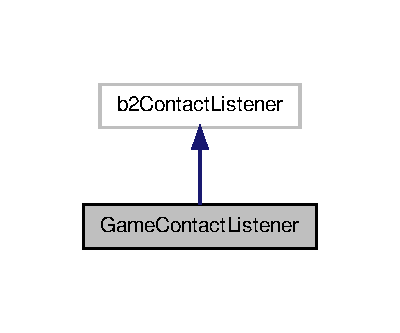
\includegraphics[width=192pt]{class_game_contact_listener__coll__graph}
\end{center}
\end{figure}
\subsection*{Public Member Functions}
\begin{DoxyCompactItemize}
\item 
void \hyperlink{class_game_contact_listener_a3a66eddc0010a96f83a0cb61d3835cc7}{Begin\-Contact} (b2\-Contact $\ast$contact)
\begin{DoxyCompactList}\small\item\em Function that allows the overload of the Begin\-Contact in the classes used in our game. \end{DoxyCompactList}\item 
void \hyperlink{class_game_contact_listener_a2d754e57a4f6c88541853a506ec3b10d}{End\-Contact} (b2\-Contact $\ast$contact)
\begin{DoxyCompactList}\small\item\em Function that allows the overload of the Begin\-Contact in the classes used in our game. \end{DoxyCompactList}\end{DoxyCompactItemize}


\subsection{Detailed Description}
Licensed to the Apache Software Foundation (A\-S\-F) under one or more contributor license agreements. See the N\-O\-T\-I\-C\-E file distributed with this work for additional information regarding copyright ownership. The A\-S\-F licenses this file to you under the Apache License, Version 2.\-0 (the \char`\"{}\-License\char`\"{}); you may not use this file except in compliance with the License. You may obtain a copy of the License at

\href{http://www.apache.org/licenses/LICENSE-2.0}{\tt http\-://www.\-apache.\-org/licenses/\-L\-I\-C\-E\-N\-S\-E-\/2.\-0}

Unless required by applicable law or agreed to in writing, software distributed under the License is distributed on an \char`\"{}\-A\-S I\-S\char`\"{} B\-A\-S\-I\-S, W\-I\-T\-H\-O\-U\-T W\-A\-R\-R\-A\-N\-T\-I\-E\-S O\-R C\-O\-N\-D\-I\-T\-I\-O\-N\-S O\-F A\-N\-Y K\-I\-N\-D, either express or implied. See the License for the specific language governing permissions and limitations under the License. File\-: \hyperlink{_game_contact_listener_8hpp_source}{Game\-Contact\-Listener.\-hpp} Creation\-: 2015-\/02-\/18 16\-:00 Vincent Rey \href{mailto:vrey@student.42.fr}{\tt vrey@student.\-42.\-fr} 

\subsection{Member Function Documentation}
\hypertarget{class_game_contact_listener_a3a66eddc0010a96f83a0cb61d3835cc7}{\index{Game\-Contact\-Listener@{Game\-Contact\-Listener}!Begin\-Contact@{Begin\-Contact}}
\index{Begin\-Contact@{Begin\-Contact}!GameContactListener@{Game\-Contact\-Listener}}
\subsubsection[{Begin\-Contact}]{\setlength{\rightskip}{0pt plus 5cm}void Game\-Contact\-Listener\-::\-Begin\-Contact (
\begin{DoxyParamCaption}
\item[{b2\-Contact $\ast$}]{contact}
\end{DoxyParamCaption}
)}}\label{class_game_contact_listener_a3a66eddc0010a96f83a0cb61d3835cc7}


Function that allows the overload of the Begin\-Contact in the classes used in our game. 

Licensed to the Apache Software Foundation (A\-S\-F) under one or more contributor license agreements. See the N\-O\-T\-I\-C\-E file distributed with this work for additional information regarding copyright ownership. The A\-S\-F licenses this file to you under the Apache License, Version 2.\-0 (the \char`\"{}\-License\char`\"{}); you may not use this file except in compliance with the License. You may obtain a copy of the License at

\href{http://www.apache.org/licenses/LICENSE-2.0}{\tt http\-://www.\-apache.\-org/licenses/\-L\-I\-C\-E\-N\-S\-E-\/2.\-0}

Unless required by applicable law or agreed to in writing, software distributed under the License is distributed on an \char`\"{}\-A\-S I\-S\char`\"{} B\-A\-S\-I\-S, W\-I\-T\-H\-O\-U\-T W\-A\-R\-R\-A\-N\-T\-I\-E\-S O\-R C\-O\-N\-D\-I\-T\-I\-O\-N\-S O\-F A\-N\-Y K\-I\-N\-D, either express or implied. See the License for the specific language governing permissions and limitations under the License. File\-: Game\-Contact\-Listener.\-cpp Creation\-: 2015-\/02-\/18 16\-:00 Vincent Rey \href{mailto:vrey@student.42.fr}{\tt vrey@student.\-42.\-fr} This function is called when a contact B\-E\-G\-I\-N\-S 
\begin{DoxyParams}{Parameters}
{\em contact} & b2\-Contact$\ast$ (See Box2\-D doc for more infos) \\
\hline
\end{DoxyParams}
\hypertarget{class_game_contact_listener_a2d754e57a4f6c88541853a506ec3b10d}{\index{Game\-Contact\-Listener@{Game\-Contact\-Listener}!End\-Contact@{End\-Contact}}
\index{End\-Contact@{End\-Contact}!GameContactListener@{Game\-Contact\-Listener}}
\subsubsection[{End\-Contact}]{\setlength{\rightskip}{0pt plus 5cm}void Game\-Contact\-Listener\-::\-End\-Contact (
\begin{DoxyParamCaption}
\item[{b2\-Contact $\ast$}]{contact}
\end{DoxyParamCaption}
)}}\label{class_game_contact_listener_a2d754e57a4f6c88541853a506ec3b10d}


Function that allows the overload of the Begin\-Contact in the classes used in our game. 

This function is called when a contact E\-N\-D\-S (a.\-k.\-a. when 2 elements stop colliding each other) 
\begin{DoxyParams}{Parameters}
{\em contact} & b2\-Contact$\ast$ (See Box2\-D doc for more infos) \\
\hline
\end{DoxyParams}


The documentation for this class was generated from the following files\-:\begin{DoxyCompactItemize}
\item 
Sources/inc/Game\-Contact\-Listener.\-hpp\item 
Sources/src/Game\-Contact\-Listener.\-cpp\end{DoxyCompactItemize}

\hypertarget{class_hero}{\section{Hero Class Reference}
\label{class_hero}\index{Hero@{Hero}}
}


{\ttfamily \#include $<$Hero.\-hpp$>$}



Inheritance diagram for Hero\-:\nopagebreak
\begin{figure}[H]
\begin{center}
\leavevmode
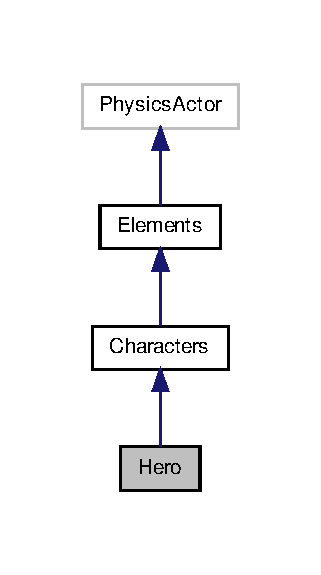
\includegraphics[width=154pt]{class_hero__inherit__graph}
\end{center}
\end{figure}


Collaboration diagram for Hero\-:\nopagebreak
\begin{figure}[H]
\begin{center}
\leavevmode
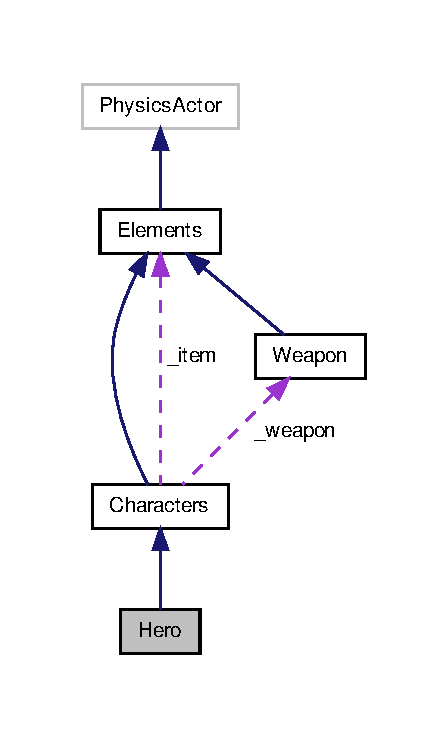
\includegraphics[width=215pt]{class_hero__coll__graph}
\end{center}
\end{figure}
\subsection*{Public Member Functions}
\begin{DoxyCompactItemize}
\item 
\hyperlink{class_hero_ab5920677a4b5cb59d6f513922d037dca}{Hero} ()
\begin{DoxyCompactList}\small\item\em Constructor. \end{DoxyCompactList}\item 
\hyperlink{class_hero_a5aeef41ede5a80dc29c5acd7b553c4da}{$\sim$\-Hero} ()
\begin{DoxyCompactList}\small\item\em Destructor. \end{DoxyCompactList}\item 
void \hyperlink{class_hero_ae67cc4b7770083755895b78664d0ea34}{init} ()
\begin{DoxyCompactList}\small\item\em Init Animation function. \end{DoxyCompactList}\item 
virtual void \hyperlink{class_hero_ac23c090d8f5e2768b4175580a0d53d1b}{Begin\-Contact} (\hyperlink{class_elements}{Elements} $\ast$m, b2\-Contact $\ast$contact)
\begin{DoxyCompactList}\small\item\em Begin collision function. \end{DoxyCompactList}\item 
virtual void \hyperlink{class_hero_a9fee92d1b0df478f95bc10ba84015d2a}{End\-Contact} (\hyperlink{class_elements}{Elements} $\ast$m, b2\-Contact $\ast$contact)
\begin{DoxyCompactList}\small\item\em End collision function. \end{DoxyCompactList}\item 
virtual void \hyperlink{class_hero_aa41ef53abd25057ceb431811ccf80ad5}{action\-Callback} (std\-::string name, int status)
\begin{DoxyCompactList}\small\item\em Action callback function. \end{DoxyCompactList}\end{DoxyCompactItemize}
\subsection*{Additional Inherited Members}


\subsection{Detailed Description}
Licensed to the Apache Software Foundation (A\-S\-F) under one or more contributor license agreements. See the N\-O\-T\-I\-C\-E file distributed with this work for additional information regarding copyright ownership. The A\-S\-F licenses this file to you under the Apache License, Version 2.\-0 (the \char`\"{}\-License\char`\"{}); you may not use this file except in compliance with the License. You may obtain a copy of the License at

\href{http://www.apache.org/licenses/LICENSE-2.0}{\tt http\-://www.\-apache.\-org/licenses/\-L\-I\-C\-E\-N\-S\-E-\/2.\-0}

Unless required by applicable law or agreed to in writing, software distributed under the License is distributed on an \char`\"{}\-A\-S I\-S\char`\"{} B\-A\-S\-I\-S, W\-I\-T\-H\-O\-U\-T W\-A\-R\-R\-A\-N\-T\-I\-E\-S O\-R C\-O\-N\-D\-I\-T\-I\-O\-N\-S O\-F A\-N\-Y K\-I\-N\-D, either express or implied. See the License for the specific language governing permissions and limitations under the License. File\-: \hyperlink{_hero_8hpp_source}{Hero.\-hpp} Creation\-: 2015-\/02-\/14 10\-:49 Louis Solofrizzo \href{mailto:louis@ne02ptzero.me}{\tt louis@ne02ptzero.\-me} 

\subsection{Constructor \& Destructor Documentation}
\hypertarget{class_hero_ab5920677a4b5cb59d6f513922d037dca}{\index{Hero@{Hero}!Hero@{Hero}}
\index{Hero@{Hero}!Hero@{Hero}}
\subsubsection[{Hero}]{\setlength{\rightskip}{0pt plus 5cm}Hero\-::\-Hero (
\begin{DoxyParamCaption}
\item[{void}]{}
\end{DoxyParamCaption}
)}}\label{class_hero_ab5920677a4b5cb59d6f513922d037dca}


Constructor. 

Licensed to the Apache Software Foundation (A\-S\-F) under one or more contributor license agreements. See the N\-O\-T\-I\-C\-E file distributed with this work for additional information regarding copyright ownership. The A\-S\-F licenses this file to you under the Apache License, Version 2.\-0 (the \char`\"{}\-License\char`\"{}); you may not use this file except in compliance with the License. You may obtain a copy of the License at

\href{http://www.apache.org/licenses/LICENSE-2.0}{\tt http\-://www.\-apache.\-org/licenses/\-L\-I\-C\-E\-N\-S\-E-\/2.\-0}

Unless required by applicable law or agreed to in writing, software distributed under the License is distributed on an \char`\"{}\-A\-S I\-S\char`\"{} B\-A\-S\-I\-S, W\-I\-T\-H\-O\-U\-T W\-A\-R\-R\-A\-N\-T\-I\-E\-S O\-R C\-O\-N\-D\-I\-T\-I\-O\-N\-S O\-F A\-N\-Y K\-I\-N\-D, either express or implied. See the License for the specific language governing permissions and limitations under the License. File\-: Hero.\-cpp Creation\-: 2015-\/02-\/14 10\-:49 Louis Solofrizzo \href{mailto:louis@ne02ptzero.me}{\tt louis@ne02ptzero.\-me} This constructor is making some subscribtions for himself. \hypertarget{class_hero_a5aeef41ede5a80dc29c5acd7b553c4da}{\index{Hero@{Hero}!$\sim$\-Hero@{$\sim$\-Hero}}
\index{$\sim$\-Hero@{$\sim$\-Hero}!Hero@{Hero}}
\subsubsection[{$\sim$\-Hero}]{\setlength{\rightskip}{0pt plus 5cm}Hero\-::$\sim$\-Hero (
\begin{DoxyParamCaption}
\item[{void}]{}
\end{DoxyParamCaption}
)}}\label{class_hero_a5aeef41ede5a80dc29c5acd7b553c4da}


Destructor. 

Basic Destructor 

\subsection{Member Function Documentation}
\hypertarget{class_hero_aa41ef53abd25057ceb431811ccf80ad5}{\index{Hero@{Hero}!action\-Callback@{action\-Callback}}
\index{action\-Callback@{action\-Callback}!Hero@{Hero}}
\subsubsection[{action\-Callback}]{\setlength{\rightskip}{0pt plus 5cm}void Hero\-::action\-Callback (
\begin{DoxyParamCaption}
\item[{std\-::string}]{name, }
\item[{int}]{status}
\end{DoxyParamCaption}
)\hspace{0.3cm}{\ttfamily [virtual]}}}\label{class_hero_aa41ef53abd25057ceb431811ccf80ad5}


Action callback function. 

Mother's callback for actions See \hyperlink{class_characters_ae6b55c4269efc485d7926f62544eef4e}{Characters\-::\-Receive\-Message} for more information. 
\begin{DoxyParams}{Parameters}
{\em } & name The action name \\
\hline
{\em } & status The key status (1 $|$ 0) \\
\hline
\end{DoxyParams}
\begin{DoxySeeAlso}{See Also}
\-: \hyperlink{class_characters_ae6b55c4269efc485d7926f62544eef4e}{Characters\-::\-Receive\-Message} 
\end{DoxySeeAlso}


Reimplemented from \hyperlink{class_characters}{Characters}.

\hypertarget{class_hero_ac23c090d8f5e2768b4175580a0d53d1b}{\index{Hero@{Hero}!Begin\-Contact@{Begin\-Contact}}
\index{Begin\-Contact@{Begin\-Contact}!Hero@{Hero}}
\subsubsection[{Begin\-Contact}]{\setlength{\rightskip}{0pt plus 5cm}void Hero\-::\-Begin\-Contact (
\begin{DoxyParamCaption}
\item[{{\bf Elements} $\ast$}]{elem, }
\item[{b2\-Contact $\ast$}]{contact}
\end{DoxyParamCaption}
)\hspace{0.3cm}{\ttfamily [virtual]}}}\label{class_hero_ac23c090d8f5e2768b4175580a0d53d1b}


Begin collision function. 

Collision begin callback /!\textbackslash{} This function is called just before a collision 
\begin{DoxyParams}{Parameters}
{\em } & elem The other Element \\
\hline
{\em } & contact The Box2\-D contact object \\
\hline
\end{DoxyParams}


Reimplemented from \hyperlink{class_characters_ae1b52f35e60cd23ec118595a9a8e8760}{Characters}.

\hypertarget{class_hero_a9fee92d1b0df478f95bc10ba84015d2a}{\index{Hero@{Hero}!End\-Contact@{End\-Contact}}
\index{End\-Contact@{End\-Contact}!Hero@{Hero}}
\subsubsection[{End\-Contact}]{\setlength{\rightskip}{0pt plus 5cm}void Hero\-::\-End\-Contact (
\begin{DoxyParamCaption}
\item[{{\bf Elements} $\ast$}]{elem, }
\item[{b2\-Contact $\ast$}]{contact}
\end{DoxyParamCaption}
)\hspace{0.3cm}{\ttfamily [virtual]}}}\label{class_hero_a9fee92d1b0df478f95bc10ba84015d2a}


End collision function. 

End contact callback. /!\textbackslash{} This function is actually called after a collision. 
\begin{DoxyParams}{Parameters}
{\em } & elem The other Element. \\
\hline
{\em contact} & The Box2\-D contact object \\
\hline
\end{DoxyParams}


Reimplemented from \hyperlink{class_characters_a87c76bb34f5c11e2da4537be07d2f846}{Characters}.

\hypertarget{class_hero_ae67cc4b7770083755895b78664d0ea34}{\index{Hero@{Hero}!init@{init}}
\index{init@{init}!Hero@{Hero}}
\subsubsection[{init}]{\setlength{\rightskip}{0pt plus 5cm}void Hero\-::init (
\begin{DoxyParamCaption}
\item[{void}]{}
\end{DoxyParamCaption}
)}}\label{class_hero_ae67cc4b7770083755895b78664d0ea34}


Init Animation function. 

This function making the first animation call. 

The documentation for this class was generated from the following files\-:\begin{DoxyCompactItemize}
\item 
Sources/inc/Hero.\-hpp\item 
Sources/src/Hero.\-cpp\end{DoxyCompactItemize}

\hypertarget{class_hitbox}{\section{Hitbox Class Reference}
\label{class_hitbox}\index{Hitbox@{Hitbox}}
}


{\ttfamily \#include $<$Hitbox.\-hpp$>$}

\subsection*{Public Member Functions}
\begin{DoxyCompactItemize}
\item 
\hyperlink{class_hitbox_a999b0be8486978b3dd7bcd001c7c3c03}{Hitbox} ()
\begin{DoxyCompactList}\small\item\em Constructor called at the beginning, parses json and creates a list containing all the hitbox listed in the files. \end{DoxyCompactList}\item 
\hyperlink{class_hitbox_aafd01dbe871f6f7f464217345bd4ca01}{$\sim$\-Hitbox} ()
\item 
b2\-Polygon\-Shape \hyperlink{class_hitbox_a2f5b5e9940cc0918e58dfbfb62a493bb}{get\-Hitbox} (std\-::string)
\begin{DoxyCompactList}\small\item\em Returns the ordered vertices in order to create the hitbox when necessary. \end{DoxyCompactList}\item 
int \hyperlink{class_hitbox_ae1b89c84071782c72ee6feb56c109c59}{check\-Exists} (std\-::string)
\begin{DoxyCompactList}\small\item\em Always return 1, cause its funnier. \end{DoxyCompactList}\end{DoxyCompactItemize}


\subsection{Detailed Description}
Licensed to the Apache Software Foundation (A\-S\-F) under one or more contributor license agreements. See the N\-O\-T\-I\-C\-E file distributed with this work for additional information regarding copyright ownership. The A\-S\-F licenses this file to you under the Apache License, Version 2.\-0 (the \char`\"{}\-License\char`\"{}); you may not use this file except in compliance with the License. You may obtain a copy of the License at

\href{http://www.apache.org/licenses/LICENSE-2.0}{\tt http\-://www.\-apache.\-org/licenses/\-L\-I\-C\-E\-N\-S\-E-\/2.\-0}

Unless required by applicable law or agreed to in writing, software distributed under the License is distributed on an \char`\"{}\-A\-S I\-S\char`\"{} B\-A\-S\-I\-S, W\-I\-T\-H\-O\-U\-T W\-A\-R\-R\-A\-N\-T\-I\-E\-S O\-R C\-O\-N\-D\-I\-T\-I\-O\-N\-S O\-F A\-N\-Y K\-I\-N\-D, either express or implied. See the License for the specific language governing permissions and limitations under the License. File\-: \hyperlink{_hitbox_8hpp_source}{Hitbox.\-hpp} Creation\-: 2015-\/02-\/27 04\-:45 Vincent Rey \href{mailto:vrey@student.42.fr}{\tt vrey@student.\-42.\-fr} 

\subsection{Constructor \& Destructor Documentation}
\hypertarget{class_hitbox_a999b0be8486978b3dd7bcd001c7c3c03}{\index{Hitbox@{Hitbox}!Hitbox@{Hitbox}}
\index{Hitbox@{Hitbox}!Hitbox@{Hitbox}}
\subsubsection[{Hitbox}]{\setlength{\rightskip}{0pt plus 5cm}Hitbox\-::\-Hitbox (
\begin{DoxyParamCaption}
\item[{void}]{}
\end{DoxyParamCaption}
)}}\label{class_hitbox_a999b0be8486978b3dd7bcd001c7c3c03}


Constructor called at the beginning, parses json and creates a list containing all the hitbox listed in the files. 

Licensed to the Apache Software Foundation (A\-S\-F) under one or more contributor license agreements. See the N\-O\-T\-I\-C\-E file distributed with this work for additional information regarding copyright ownership. The A\-S\-F licenses this file to you under the Apache License, Version 2.\-0 (the \char`\"{}\-License\char`\"{}); you may not use this file except in compliance with the License. You may obtain a copy of the License at

\href{http://www.apache.org/licenses/LICENSE-2.0}{\tt http\-://www.\-apache.\-org/licenses/\-L\-I\-C\-E\-N\-S\-E-\/2.\-0}

Unless required by applicable law or agreed to in writing, software distributed under the License is distributed on an \char`\"{}\-A\-S I\-S\char`\"{} B\-A\-S\-I\-S, W\-I\-T\-H\-O\-U\-T W\-A\-R\-R\-A\-N\-T\-I\-E\-S O\-R C\-O\-N\-D\-I\-T\-I\-O\-N\-S O\-F A\-N\-Y K\-I\-N\-D, either express or implied. See the License for the specific language governing permissions and limitations under the License. File\-: Hitbox.\-cpp Creation\-: 2015-\/02-\/18 14\-:00 Vincent Rey \href{mailto:vrey@student.42.fr}{\tt vrey@student.\-42.\-fr} Default constructor, creating the list /!\textbackslash{} General warning\-: /!\textbackslash{} Box2\-D hitbox creator does not allow \-: concave polygons, less-\/than-\/four vertices polygons (aka triangles), more-\/than-\/eight vertices polygons /!\textbackslash{} The game will either not start or crash during startup if one of theses is attempted \hypertarget{class_hitbox_aafd01dbe871f6f7f464217345bd4ca01}{\index{Hitbox@{Hitbox}!$\sim$\-Hitbox@{$\sim$\-Hitbox}}
\index{$\sim$\-Hitbox@{$\sim$\-Hitbox}!Hitbox@{Hitbox}}
\subsubsection[{$\sim$\-Hitbox}]{\setlength{\rightskip}{0pt plus 5cm}Hitbox\-::$\sim$\-Hitbox (
\begin{DoxyParamCaption}
\item[{void}]{}
\end{DoxyParamCaption}
)}}\label{class_hitbox_aafd01dbe871f6f7f464217345bd4ca01}
Basic destructor 

\subsection{Member Function Documentation}
\hypertarget{class_hitbox_ae1b89c84071782c72ee6feb56c109c59}{\index{Hitbox@{Hitbox}!check\-Exists@{check\-Exists}}
\index{check\-Exists@{check\-Exists}!Hitbox@{Hitbox}}
\subsubsection[{check\-Exists}]{\setlength{\rightskip}{0pt plus 5cm}int Hitbox\-::check\-Exists (
\begin{DoxyParamCaption}
\item[{std\-::string}]{n}
\end{DoxyParamCaption}
)}}\label{class_hitbox_ae1b89c84071782c72ee6feb56c109c59}


Always return 1, cause its funnier. 

Function that checks if requested hitbox does exists, as the object cannot be null 
\begin{DoxyParams}{Parameters}
{\em n} & std\-::string (name of the hitbox) Do not call get\-Hitbox if this function returns false \\
\hline
\end{DoxyParams}
\begin{DoxyRefDesc}{Todo}
\item[\hyperlink{todo__todo000007}{Todo}]\-: yeah... \end{DoxyRefDesc}
\hypertarget{class_hitbox_a2f5b5e9940cc0918e58dfbfb62a493bb}{\index{Hitbox@{Hitbox}!get\-Hitbox@{get\-Hitbox}}
\index{get\-Hitbox@{get\-Hitbox}!Hitbox@{Hitbox}}
\subsubsection[{get\-Hitbox}]{\setlength{\rightskip}{0pt plus 5cm}b2\-Polygon\-Shape Hitbox\-::get\-Hitbox (
\begin{DoxyParamCaption}
\item[{std\-::string}]{n}
\end{DoxyParamCaption}
)}}\label{class_hitbox_a2f5b5e9940cc0918e58dfbfb62a493bb}


Returns the ordered vertices in order to create the hitbox when necessary. 

Called mostly by characters, weapons, or objects to load a pre-\/designed hitbox 
\begin{DoxyParams}{Parameters}
{\em n} & std\-::string (name of the hitbox) \\
\hline
\end{DoxyParams}


The documentation for this class was generated from the following files\-:\begin{DoxyCompactItemize}
\item 
Sources/inc/Hitbox.\-hpp\item 
Sources/src/Hitbox.\-cpp\end{DoxyCompactItemize}

\hypertarget{class_h_u_d_window}{\section{H\-U\-D\-Window Class Reference}
\label{class_h_u_d_window}\index{H\-U\-D\-Window@{H\-U\-D\-Window}}
}


{\ttfamily \#include $<$H\-U\-D\-Window.\-hpp$>$}



Inheritance diagram for H\-U\-D\-Window\-:\nopagebreak
\begin{figure}[H]
\begin{center}
\leavevmode
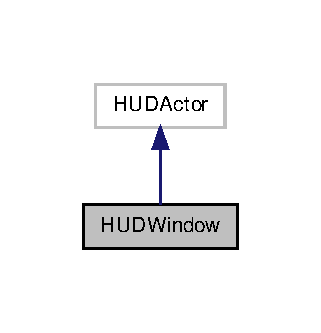
\includegraphics[width=154pt]{class_h_u_d_window__inherit__graph}
\end{center}
\end{figure}


Collaboration diagram for H\-U\-D\-Window\-:\nopagebreak
\begin{figure}[H]
\begin{center}
\leavevmode
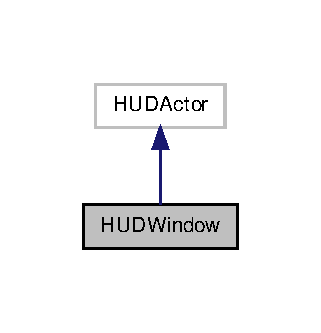
\includegraphics[width=154pt]{class_h_u_d_window__coll__graph}
\end{center}
\end{figure}
\subsection*{Public Member Functions}
\begin{DoxyCompactItemize}
\item 
\hyperlink{class_h_u_d_window_a8d97402012deb77be8008cfed176fdd6}{H\-U\-D\-Window} (void)
\begin{DoxyCompactList}\small\item\em Constructor. \end{DoxyCompactList}\item 
\hyperlink{class_h_u_d_window_ac1c288c91430729735038fcefc4bcdb8}{$\sim$\-H\-U\-D\-Window} (void)
\begin{DoxyCompactList}\small\item\em Destructor. \end{DoxyCompactList}\item 
void \hyperlink{class_h_u_d_window_a77a524e42af9d069137b70a1e5653df1}{set\-Text} (std\-::string str, int x, int y)
\begin{DoxyCompactList}\small\item\em Set text function. \end{DoxyCompactList}\item 
void \hyperlink{class_h_u_d_window_ade8fc1411dee1078b26498370bbef672}{set\-Text} (std\-::string str, int x, int y, Vector3 color, int alpha)
\begin{DoxyCompactList}\small\item\em Set text function. \end{DoxyCompactList}\item 
void \hyperlink{class_h_u_d_window_a0aedfd1f3c8354da1b69f1b592d4ad3e}{remove\-Text} (std\-::string str)
\begin{DoxyCompactList}\small\item\em Remove Text. \end{DoxyCompactList}\item 
void \hyperlink{class_h_u_d_window_a12148d8845eaa5a663d816a4befba0dd}{display\-Text} (void)
\begin{DoxyCompactList}\small\item\em Callback for Display text. \end{DoxyCompactList}\item 
void \hyperlink{class_h_u_d_window_a94366d6f68535133a56d0b38228460e0}{add\-Image} (std\-::string p, int x, int y)
\begin{DoxyCompactList}\small\item\em Add an Image. \end{DoxyCompactList}\item 
void \hyperlink{class_h_u_d_window_aee140416af161a6d8acc2b0c83370088}{add\-Image} (std\-::string path, int x, int y, float size)
\begin{DoxyCompactList}\small\item\em Add an image. \end{DoxyCompactList}\item 
void \hyperlink{class_h_u_d_window_a8fc917fbfae792d046e90448c963100a}{life} (int l)
\begin{DoxyCompactList}\small\item\em Display H\-P function. \end{DoxyCompactList}\item 
void \hyperlink{class_h_u_d_window_a6eb79b572849709a329e65ed2afd2e9e}{mana} (int mana)
\begin{DoxyCompactList}\small\item\em Display mana function. \end{DoxyCompactList}\item 
void \hyperlink{class_h_u_d_window_a4eb34de71e2ea671f637381ac255edab}{gold} (int g)
\begin{DoxyCompactList}\small\item\em Display gold function. \end{DoxyCompactList}\item 
void \hyperlink{class_h_u_d_window_a9edf25a0b1cf568aa3f338281d81d99a}{items} (\hyperlink{class_weapon}{Weapon} $\ast$w)
\begin{DoxyCompactList}\small\item\em Display items (\hyperlink{class_weapon}{Weapon}) \end{DoxyCompactList}\item 
void \hyperlink{class_h_u_d_window_a1c6965adb9fdd22b230d20b26fef5ac0}{armor} (void)
\begin{DoxyCompactList}\small\item\em Display armor. \end{DoxyCompactList}\item 
void \hyperlink{class_h_u_d_window_acd4fdbfd1c2562384b84d3bcda80fea1}{boots} (void)
\begin{DoxyCompactList}\small\item\em Display boots function. \end{DoxyCompactList}\item 
void \hyperlink{class_h_u_d_window_a378bc8269cacb151f68cfb37114e0c38}{consumable} (void)
\begin{DoxyCompactList}\small\item\em Show the consumable function. \end{DoxyCompactList}\item 
void \hyperlink{class_h_u_d_window_a8264836f3c55d8211f4e5166e9049628}{minimap} (void)
\begin{DoxyCompactList}\small\item\em Display the minimap in the H\-Ud. \end{DoxyCompactList}\item 
void \hyperlink{class_h_u_d_window_a5baefc7b585437df2639fda359c3cf46}{set\-Game} (\hyperlink{class_game}{Game} $\ast$)
\end{DoxyCompactItemize}


\subsection{Constructor \& Destructor Documentation}
\hypertarget{class_h_u_d_window_a8d97402012deb77be8008cfed176fdd6}{\index{H\-U\-D\-Window@{H\-U\-D\-Window}!H\-U\-D\-Window@{H\-U\-D\-Window}}
\index{H\-U\-D\-Window@{H\-U\-D\-Window}!HUDWindow@{H\-U\-D\-Window}}
\subsubsection[{H\-U\-D\-Window}]{\setlength{\rightskip}{0pt plus 5cm}H\-U\-D\-Window\-::\-H\-U\-D\-Window (
\begin{DoxyParamCaption}
\item[{void}]{}
\end{DoxyParamCaption}
)}}\label{class_h_u_d_window_a8d97402012deb77be8008cfed176fdd6}


Constructor. 

Licensed to the Apache Software Foundation (A\-S\-F) under one or more contributor license agreements. See the N\-O\-T\-I\-C\-E file distributed with this work for additional information regarding copyright ownership. The A\-S\-F licenses this file to you under the Apache License, Version 2.\-0 (the \char`\"{}\-License\char`\"{}); you may not use this file except in compliance with the License. You may obtain a copy of the License at

\href{http://www.apache.org/licenses/LICENSE-2.0}{\tt http\-://www.\-apache.\-org/licenses/\-L\-I\-C\-E\-N\-S\-E-\/2.\-0}

Unless required by applicable law or agreed to in writing, software distributed under the License is distributed on an \char`\"{}\-A\-S I\-S\char`\"{} B\-A\-S\-I\-S, W\-I\-T\-H\-O\-U\-T W\-A\-R\-R\-A\-N\-T\-I\-E\-S O\-R C\-O\-N\-D\-I\-T\-I\-O\-N\-S O\-F A\-N\-Y K\-I\-N\-D, either express or implied. See the License for the specific language governing permissions and limitations under the License. File\-: \hyperlink{_h_u_d_window_8cpp}{H\-U\-D\-Window.\-cpp} Creation\-: 2015-\/03-\/14 05\-:35 Louis Solofrizzo \href{mailto:louis@ne02ptzero.me}{\tt louis@ne02ptzero.\-me} Basic constructor \hypertarget{class_h_u_d_window_ac1c288c91430729735038fcefc4bcdb8}{\index{H\-U\-D\-Window@{H\-U\-D\-Window}!$\sim$\-H\-U\-D\-Window@{$\sim$\-H\-U\-D\-Window}}
\index{$\sim$\-H\-U\-D\-Window@{$\sim$\-H\-U\-D\-Window}!HUDWindow@{H\-U\-D\-Window}}
\subsubsection[{$\sim$\-H\-U\-D\-Window}]{\setlength{\rightskip}{0pt plus 5cm}H\-U\-D\-Window\-::$\sim$\-H\-U\-D\-Window (
\begin{DoxyParamCaption}
\item[{void}]{}
\end{DoxyParamCaption}
)}}\label{class_h_u_d_window_ac1c288c91430729735038fcefc4bcdb8}


Destructor. 

Basic destructor 

\subsection{Member Function Documentation}
\hypertarget{class_h_u_d_window_a94366d6f68535133a56d0b38228460e0}{\index{H\-U\-D\-Window@{H\-U\-D\-Window}!add\-Image@{add\-Image}}
\index{add\-Image@{add\-Image}!HUDWindow@{H\-U\-D\-Window}}
\subsubsection[{add\-Image}]{\setlength{\rightskip}{0pt plus 5cm}void H\-U\-D\-Window\-::add\-Image (
\begin{DoxyParamCaption}
\item[{std\-::string}]{path, }
\item[{int}]{x, }
\item[{int}]{y}
\end{DoxyParamCaption}
)}}\label{class_h_u_d_window_a94366d6f68535133a56d0b38228460e0}


Add an Image. 

Add an image in the H\-U\-D 
\begin{DoxyParams}{Parameters}
{\em } & path The path of the img \\
\hline
{\em } & x X position \\
\hline
{\em } & y Y position \\
\hline
\end{DoxyParams}
\hypertarget{class_h_u_d_window_aee140416af161a6d8acc2b0c83370088}{\index{H\-U\-D\-Window@{H\-U\-D\-Window}!add\-Image@{add\-Image}}
\index{add\-Image@{add\-Image}!HUDWindow@{H\-U\-D\-Window}}
\subsubsection[{add\-Image}]{\setlength{\rightskip}{0pt plus 5cm}void H\-U\-D\-Window\-::add\-Image (
\begin{DoxyParamCaption}
\item[{std\-::string}]{path, }
\item[{int}]{x, }
\item[{int}]{y, }
\item[{float}]{size}
\end{DoxyParamCaption}
)}}\label{class_h_u_d_window_aee140416af161a6d8acc2b0c83370088}


Add an image. 

Add an image in the H\-U\-D 
\begin{DoxyParams}{Parameters}
{\em } & path The path of the img \\
\hline
{\em } & x X position \\
\hline
{\em } & y Y position \\
\hline
{\em } & size Size, in float. \\
\hline
\end{DoxyParams}
\hypertarget{class_h_u_d_window_a1c6965adb9fdd22b230d20b26fef5ac0}{\index{H\-U\-D\-Window@{H\-U\-D\-Window}!armor@{armor}}
\index{armor@{armor}!HUDWindow@{H\-U\-D\-Window}}
\subsubsection[{armor}]{\setlength{\rightskip}{0pt plus 5cm}void H\-U\-D\-Window\-::armor (
\begin{DoxyParamCaption}
\item[{void}]{}
\end{DoxyParamCaption}
)}}\label{class_h_u_d_window_a1c6965adb9fdd22b230d20b26fef5ac0}


Display armor. 

Display the armor function. This function is a callback call in Character\-::set\-Armor. So you won't problably call this function ! \begin{DoxyRefDesc}{Todo}
\item[\hyperlink{todo__todo000007}{Todo}]\-: The description here is a lie. But it's gonna append ! \end{DoxyRefDesc}
\hypertarget{class_h_u_d_window_acd4fdbfd1c2562384b84d3bcda80fea1}{\index{H\-U\-D\-Window@{H\-U\-D\-Window}!boots@{boots}}
\index{boots@{boots}!HUDWindow@{H\-U\-D\-Window}}
\subsubsection[{boots}]{\setlength{\rightskip}{0pt plus 5cm}void H\-U\-D\-Window\-::boots (
\begin{DoxyParamCaption}
\item[{void}]{}
\end{DoxyParamCaption}
)}}\label{class_h_u_d_window_acd4fdbfd1c2562384b84d3bcda80fea1}


Display boots function. 

Show the actual boots in the \hyperlink{class_h_u_d_window}{H\-U\-D\-Window} \begin{DoxyRefDesc}{Todo}
\item[\hyperlink{todo__todo000008}{Todo}]\-: No callback \& object for now, but have to do it ! \end{DoxyRefDesc}
\hypertarget{class_h_u_d_window_a378bc8269cacb151f68cfb37114e0c38}{\index{H\-U\-D\-Window@{H\-U\-D\-Window}!consumable@{consumable}}
\index{consumable@{consumable}!HUDWindow@{H\-U\-D\-Window}}
\subsubsection[{consumable}]{\setlength{\rightskip}{0pt plus 5cm}void H\-U\-D\-Window\-::consumable (
\begin{DoxyParamCaption}
\item[{void}]{}
\end{DoxyParamCaption}
)}}\label{class_h_u_d_window_a378bc8269cacb151f68cfb37114e0c38}


Show the consumable function. 

Display the consumable (potions, etc) in the H\-U\-D \begin{DoxyRefDesc}{Todo}
\item[\hyperlink{todo__todo000009}{Todo}]\-: Same here, no callback or object. \end{DoxyRefDesc}
\hypertarget{class_h_u_d_window_a12148d8845eaa5a663d816a4befba0dd}{\index{H\-U\-D\-Window@{H\-U\-D\-Window}!display\-Text@{display\-Text}}
\index{display\-Text@{display\-Text}!HUDWindow@{H\-U\-D\-Window}}
\subsubsection[{display\-Text}]{\setlength{\rightskip}{0pt plus 5cm}void H\-U\-D\-Window\-::display\-Text (
\begin{DoxyParamCaption}
\item[{void}]{}
\end{DoxyParamCaption}
)}}\label{class_h_u_d_window_a12148d8845eaa5a663d816a4befba0dd}


Callback for Display text. 

Display a text in the H\-U\-D This function is an intern callback between \hyperlink{class_game}{Game} and \hyperlink{class_h_u_d_window}{H\-U\-D\-Window}. You problably don't want to call it. \hypertarget{class_h_u_d_window_a4eb34de71e2ea671f637381ac255edab}{\index{H\-U\-D\-Window@{H\-U\-D\-Window}!gold@{gold}}
\index{gold@{gold}!HUDWindow@{H\-U\-D\-Window}}
\subsubsection[{gold}]{\setlength{\rightskip}{0pt plus 5cm}void H\-U\-D\-Window\-::gold (
\begin{DoxyParamCaption}
\item[{int}]{gold}
\end{DoxyParamCaption}
)}}\label{class_h_u_d_window_a4eb34de71e2ea671f637381ac255edab}


Display gold function. 

Make it rain baby Like this all A\-P\-I, evrything his handled. Don't worry. 
\begin{DoxyParams}{Parameters}
{\em } & gold The gold number \\
\hline
\end{DoxyParams}
\hypertarget{class_h_u_d_window_a9edf25a0b1cf568aa3f338281d81d99a}{\index{H\-U\-D\-Window@{H\-U\-D\-Window}!items@{items}}
\index{items@{items}!HUDWindow@{H\-U\-D\-Window}}
\subsubsection[{items}]{\setlength{\rightskip}{0pt plus 5cm}void H\-U\-D\-Window\-::items (
\begin{DoxyParamCaption}
\item[{{\bf Weapon} $\ast$}]{w}
\end{DoxyParamCaption}
)}}\label{class_h_u_d_window_a9edf25a0b1cf568aa3f338281d81d99a}


Display items (\hyperlink{class_weapon}{Weapon}) 

Display the weapon function. This function is a callback call in Character\-::set\-Weapon. So you won't problably call this function ! 
\begin{DoxyParams}{Parameters}
{\em } & w The \hyperlink{class_weapon}{Weapon} equipped. \\
\hline
\end{DoxyParams}
\hypertarget{class_h_u_d_window_a8fc917fbfae792d046e90448c963100a}{\index{H\-U\-D\-Window@{H\-U\-D\-Window}!life@{life}}
\index{life@{life}!HUDWindow@{H\-U\-D\-Window}}
\subsubsection[{life}]{\setlength{\rightskip}{0pt plus 5cm}void H\-U\-D\-Window\-::life (
\begin{DoxyParamCaption}
\item[{int}]{life}
\end{DoxyParamCaption}
)}}\label{class_h_u_d_window_a8fc917fbfae792d046e90448c963100a}


Display H\-P function. 

Life is life (lalala) This function take care of the heart, in the H\-U\-D. 
\begin{DoxyParams}{Parameters}
{\em } & int The life number \\
\hline
\end{DoxyParams}
\begin{DoxyRefDesc}{Todo}
\item[\hyperlink{todo__todo000006}{Todo}]\-: Empty heart, half-\/heart. \end{DoxyRefDesc}
\hypertarget{class_h_u_d_window_a6eb79b572849709a329e65ed2afd2e9e}{\index{H\-U\-D\-Window@{H\-U\-D\-Window}!mana@{mana}}
\index{mana@{mana}!HUDWindow@{H\-U\-D\-Window}}
\subsubsection[{mana}]{\setlength{\rightskip}{0pt plus 5cm}void H\-U\-D\-Window\-::mana (
\begin{DoxyParamCaption}
\item[{int}]{mana}
\end{DoxyParamCaption}
)}}\label{class_h_u_d_window_a6eb79b572849709a329e65ed2afd2e9e}


Display mana function. 

Show the mana in the H\-U\-D Same way as \hyperlink{class_h_u_d_window_a8fc917fbfae792d046e90448c963100a}{H\-U\-D\-Window\-::life}, this function handle the sprites, and the Empty mana 
\begin{DoxyParams}{Parameters}
{\em } & mana The Mana point. \\
\hline
\end{DoxyParams}
\hypertarget{class_h_u_d_window_a8264836f3c55d8211f4e5166e9049628}{\index{H\-U\-D\-Window@{H\-U\-D\-Window}!minimap@{minimap}}
\index{minimap@{minimap}!HUDWindow@{H\-U\-D\-Window}}
\subsubsection[{minimap}]{\setlength{\rightskip}{0pt plus 5cm}void H\-U\-D\-Window\-::minimap (
\begin{DoxyParamCaption}
\item[{void}]{}
\end{DoxyParamCaption}
)}}\label{class_h_u_d_window_a8264836f3c55d8211f4e5166e9049628}


Display the minimap in the H\-Ud. 

This function is not finished at all. So don't use it. Thank's. \begin{DoxyRefDesc}{Todo}
\item[\hyperlink{todo__todo000010}{Todo}]\-: Make this function work normally. \end{DoxyRefDesc}
\hypertarget{class_h_u_d_window_a0aedfd1f3c8354da1b69f1b592d4ad3e}{\index{H\-U\-D\-Window@{H\-U\-D\-Window}!remove\-Text@{remove\-Text}}
\index{remove\-Text@{remove\-Text}!HUDWindow@{H\-U\-D\-Window}}
\subsubsection[{remove\-Text}]{\setlength{\rightskip}{0pt plus 5cm}void H\-U\-D\-Window\-::remove\-Text (
\begin{DoxyParamCaption}
\item[{std\-::string}]{str}
\end{DoxyParamCaption}
)}}\label{class_h_u_d_window_a0aedfd1f3c8354da1b69f1b592d4ad3e}


Remove Text. 

This function remove the asked text from the screen. 
\begin{DoxyParams}{Parameters}
{\em } & str The text content message \\
\hline
\end{DoxyParams}
\hypertarget{class_h_u_d_window_a5baefc7b585437df2639fda359c3cf46}{\index{H\-U\-D\-Window@{H\-U\-D\-Window}!set\-Game@{set\-Game}}
\index{set\-Game@{set\-Game}!HUDWindow@{H\-U\-D\-Window}}
\subsubsection[{set\-Game}]{\setlength{\rightskip}{0pt plus 5cm}void H\-U\-D\-Window\-::set\-Game (
\begin{DoxyParamCaption}
\item[{{\bf Game} $\ast$}]{g}
\end{DoxyParamCaption}
)}}\label{class_h_u_d_window_a5baefc7b585437df2639fda359c3cf46}
\hypertarget{class_h_u_d_window_a77a524e42af9d069137b70a1e5653df1}{\index{H\-U\-D\-Window@{H\-U\-D\-Window}!set\-Text@{set\-Text}}
\index{set\-Text@{set\-Text}!HUDWindow@{H\-U\-D\-Window}}
\subsubsection[{set\-Text}]{\setlength{\rightskip}{0pt plus 5cm}void H\-U\-D\-Window\-::set\-Text (
\begin{DoxyParamCaption}
\item[{std\-::string}]{str, }
\item[{int}]{x, }
\item[{int}]{y}
\end{DoxyParamCaption}
)}}\label{class_h_u_d_window_a77a524e42af9d069137b70a1e5653df1}


Set text function. 

Set a text in the window 
\begin{DoxyParams}{Parameters}
{\em } & str The text message \\
\hline
{\em } & x X position \\
\hline
{\em } & y Y position \\
\hline
\end{DoxyParams}
\hypertarget{class_h_u_d_window_ade8fc1411dee1078b26498370bbef672}{\index{H\-U\-D\-Window@{H\-U\-D\-Window}!set\-Text@{set\-Text}}
\index{set\-Text@{set\-Text}!HUDWindow@{H\-U\-D\-Window}}
\subsubsection[{set\-Text}]{\setlength{\rightskip}{0pt plus 5cm}void H\-U\-D\-Window\-::set\-Text (
\begin{DoxyParamCaption}
\item[{std\-::string}]{str, }
\item[{int}]{x, }
\item[{int}]{y, }
\item[{Vector3}]{color, }
\item[{int}]{alpha}
\end{DoxyParamCaption}
)}}\label{class_h_u_d_window_ade8fc1411dee1078b26498370bbef672}


Set text function. 

Set a text in the window 
\begin{DoxyParams}{Parameters}
{\em } & str The text message \\
\hline
{\em } & x X position \\
\hline
{\em } & y Y position \\
\hline
{\em } & color The color of the text (See Angel2d's Vector3 for more info) \\
\hline
{\em } & alpha The transparency. \\
\hline
\end{DoxyParams}


The documentation for this class was generated from the following files\-:\begin{DoxyCompactItemize}
\item 
/home/louis/\-Documents/rogue-\/like/\-Sources/inc/\hyperlink{_h_u_d_window_8hpp}{H\-U\-D\-Window.\-hpp}\item 
/home/louis/\-Documents/rogue-\/like/\-Sources/src/\hyperlink{_h_u_d_window_8cpp}{H\-U\-D\-Window.\-cpp}\end{DoxyCompactItemize}

\hypertarget{class_level_generator}{\section{Level\+Generator Class Reference}
\label{class_level_generator}\index{Level\+Generator@{Level\+Generator}}
}


{\ttfamily \#include $<$Level\+Generator.\+hpp$>$}

\subsection*{Public Member Functions}
\begin{DoxyCompactItemize}
\item 
\hyperlink{class_level_generator_ad509b6dd7dbfd144466315ce2c493513}{Level\+Generator} (int max\+Map\+Size, int min\+Path\+Lenght, int doors\+Pop\+Rate)
\item 
\hyperlink{class_level_generator_a9bd612e10a3d769537ba042a76c0cb5f}{$\sim$\+Level\+Generator} ()
\item 
\hypertarget{class_level_generator_ad3a873efd53cec998e5b3cbec90b1e6d}{void {\bfseries print} (void)}\label{class_level_generator_ad3a873efd53cec998e5b3cbec90b1e6d}

\item 
\hypertarget{class_level_generator_aabdbf98d1f6b41ef3f921c7c08bac691}{void {\bfseries execute} (void)}\label{class_level_generator_aabdbf98d1f6b41ef3f921c7c08bac691}

\item 
\hypertarget{class_level_generator_a3a3c144dfccee44c67f42da9ad77ca93}{void {\bfseries create\+First\+Room} (void)}\label{class_level_generator_a3a3c144dfccee44c67f42da9ad77ca93}

\item 
\hypertarget{class_level_generator_a1f333c183a88620a11fa542067408184}{void {\bfseries first\+Pass} (int distance)}\label{class_level_generator_a1f333c183a88620a11fa542067408184}

\item 
\hypertarget{class_level_generator_a9d352262bacb1e8505ed1f2c76266555}{void {\bfseries generate\+Rooms\+Behind\+Doors} (\hyperlink{class_room}{Room} $\ast$room)}\label{class_level_generator_a9d352262bacb1e8505ed1f2c76266555}

\item 
\hypertarget{class_level_generator_aabd2f2b813e71976ce760304ddd401d6}{\hyperlink{class_room}{Room} $\ast$ {\bfseries generate\+Room} (int x, int y, int distance, \hyperlink{class_room}{Room} $\ast$prev\+Room, int origin)}\label{class_level_generator_aabd2f2b813e71976ce760304ddd401d6}

\item 
\hypertarget{class_level_generator_aa8297433f2d818a0e1839faf9c899f4d}{bool {\bfseries test\+Door} (int x, int y)}\label{class_level_generator_aa8297433f2d818a0e1839faf9c899f4d}

\item 
\hypertarget{class_level_generator_a4ea22d65b574c874fdf8d1480dfb7ceb}{bool {\bfseries test\+Room} (int x, int y)}\label{class_level_generator_a4ea22d65b574c874fdf8d1480dfb7ceb}

\item 
\hypertarget{class_level_generator_aaaccd1f1c3b4331d30ba5a56b3d027f8}{void {\bfseries link\+Adjacent\+Rooms} (\hyperlink{class_room}{Room} $\ast$room)}\label{class_level_generator_aaaccd1f1c3b4331d30ba5a56b3d027f8}

\item 
\hypertarget{class_level_generator_ae7e5462d7434108c2ef3ae9c217a29c8}{void {\bfseries shockwave} (void)}\label{class_level_generator_ae7e5462d7434108c2ef3ae9c217a29c8}

\item 
\hypertarget{class_level_generator_a4a54eac0ab907095552548bf67a5aa55}{int {\bfseries get\+Entry\+Id} (void)}\label{class_level_generator_a4a54eac0ab907095552548bf67a5aa55}

\item 
\hypertarget{class_level_generator_af415fc7e70da9af9d8b3cae64988e3db}{int {\bfseries id} (void)}\label{class_level_generator_af415fc7e70da9af9d8b3cae64988e3db}

\item 
\hypertarget{class_level_generator_a2a1aaa623b0fbb7c08a37b233bc0eddc}{std\+::vector$<$ std\+::vector$<$ int $>$ $>$ {\bfseries get\+Level} (void)}\label{class_level_generator_a2a1aaa623b0fbb7c08a37b233bc0eddc}

\item 
\hypertarget{class_level_generator_adc1012bf21a7bff0887cc3e74b8f18f1}{int {\bfseries get\+Start\+X} ()}\label{class_level_generator_adc1012bf21a7bff0887cc3e74b8f18f1}

\item 
\hypertarget{class_level_generator_a2724eb94a1f8a3c2cb96d284eddeab0f}{int {\bfseries get\+Start\+Y} ()}\label{class_level_generator_a2724eb94a1f8a3c2cb96d284eddeab0f}

\item 
\hypertarget{class_level_generator_ae198cc8f678e6bb3f51932099dc5f6c9}{int {\bfseries get\+Nb\+Maps} ()}\label{class_level_generator_ae198cc8f678e6bb3f51932099dc5f6c9}

\end{DoxyCompactItemize}
\subsection*{Public Attributes}
\begin{DoxyCompactItemize}
\item 
\hypertarget{class_level_generator_aaeb382a82733c6d95569b9b77c0c3b11}{std\+::vector$<$ \hyperlink{class_room}{Room} $\ast$ $>$ $\ast$ {\bfseries \+\_\+rooms}}\label{class_level_generator_aaeb382a82733c6d95569b9b77c0c3b11}

\end{DoxyCompactItemize}


\subsection{Detailed Description}
Licensed to the Apache Software Foundation (A\+S\+F) under one or more contributor license agreements. See the N\+O\+T\+I\+C\+E file distributed with this work for additional information regarding copyright ownership. The A\+S\+F licenses this file to you under the Apache License, Version 2.\+0 (the \char`\"{}\+License\char`\"{}); you may not use this file except in compliance with the License. You may obtain a copy of the License at

\href{http://www.apache.org/licenses/LICENSE-2.0}{\tt http\+://www.\+apache.\+org/licenses/\+L\+I\+C\+E\+N\+S\+E-\/2.\+0}

Unless required by applicable law or agreed to in writing, software distributed under the License is distributed on an \char`\"{}\+A\+S I\+S\char`\"{} B\+A\+S\+I\+S, W\+I\+T\+H\+O\+U\+T W\+A\+R\+R\+A\+N\+T\+I\+E\+S O\+R C\+O\+N\+D\+I\+T\+I\+O\+N\+S O\+F A\+N\+Y K\+I\+N\+D, either express or implied. See the License for the specific language governing permissions and limitations under the License. File\+: \hyperlink{_level_generator_8hpp_source}{Level\+Generator.\+hpp} Creation\+: 2015-\/03-\/02 16\+:05 Matthieu Maudet \href{mailto:mmaudet@student.42.fr}{\tt mmaudet@student.\+42.\+fr} 

\subsection{Constructor \& Destructor Documentation}
\hypertarget{class_level_generator_ad509b6dd7dbfd144466315ce2c493513}{\index{Level\+Generator@{Level\+Generator}!Level\+Generator@{Level\+Generator}}
\index{Level\+Generator@{Level\+Generator}!Level\+Generator@{Level\+Generator}}
\subsubsection[{Level\+Generator}]{\setlength{\rightskip}{0pt plus 5cm}Level\+Generator\+::\+Level\+Generator (
\begin{DoxyParamCaption}
\item[{int}]{max\+Map\+Size, }
\item[{int}]{min\+Path\+Lenght, }
\item[{int}]{doors\+Pop\+Rate}
\end{DoxyParamCaption}
)}}\label{class_level_generator_ad509b6dd7dbfd144466315ce2c493513}
Licensed to the Apache Software Foundation (A\+S\+F) under one or more contributor license agreements. See the N\+O\+T\+I\+C\+E file distributed with this work for additional information regarding copyright ownership. The A\+S\+F licenses this file to you under the Apache License, Version 2.\+0 (the \char`\"{}\+License\char`\"{}); you may not use this file except in compliance with the License. You may obtain a copy of the License at

\href{http://www.apache.org/licenses/LICENSE-2.0}{\tt http\+://www.\+apache.\+org/licenses/\+L\+I\+C\+E\+N\+S\+E-\/2.\+0}

Unless required by applicable law or agreed to in writing, software distributed under the License is distributed on an \char`\"{}\+A\+S I\+S\char`\"{} B\+A\+S\+I\+S, W\+I\+T\+H\+O\+U\+T W\+A\+R\+R\+A\+N\+T\+I\+E\+S O\+R C\+O\+N\+D\+I\+T\+I\+O\+N\+S O\+F A\+N\+Y K\+I\+N\+D, either express or implied. See the License for the specific language governing permissions and limitations under the License. File\+: Level\+Generator.\+cpp Creation\+: 2015-\/03-\/02 16\+:05 Matthieu Maudet \href{mailto:mmaudet@student.42.fr}{\tt mmaudet@student.\+42.\+fr} Standard constructor with \+:
\begin{DoxyItemize}
\item Height and Width
\item min\+Path\+Lenght \+: Min path between entry and exit rooms
\item room\+Pop\+Rate (of 100\%) \+: Chances for a room to pop on given slot
\item doors\+Pop\+Rate (of 100\%) \+: Chances for a door to pop on given wall
\item nb\+Maps \+: Number of different maps 
\end{DoxyItemize}\hypertarget{class_level_generator_a9bd612e10a3d769537ba042a76c0cb5f}{\index{Level\+Generator@{Level\+Generator}!````~Level\+Generator@{$\sim$\+Level\+Generator}}
\index{````~Level\+Generator@{$\sim$\+Level\+Generator}!Level\+Generator@{Level\+Generator}}
\subsubsection[{$\sim$\+Level\+Generator}]{\setlength{\rightskip}{0pt plus 5cm}Level\+Generator\+::$\sim$\+Level\+Generator (
\begin{DoxyParamCaption}
\item[{void}]{}
\end{DoxyParamCaption}
)}}\label{class_level_generator_a9bd612e10a3d769537ba042a76c0cb5f}
Basic Destructor 

The documentation for this class was generated from the following files\+:\begin{DoxyCompactItemize}
\item 
Sources/inc/Level\+Generator.\+hpp\item 
Sources/src/Level\+Generator.\+cpp\end{DoxyCompactItemize}

\hypertarget{class_log}{\section{Log Class Reference}
\label{class_log}\index{Log@{Log}}
}


{\ttfamily \#include $<$Log.\-hpp$>$}

\subsection*{Public Member Functions}
\begin{DoxyCompactItemize}
\item 
\hyperlink{class_log_af6071a60aa52b6c1b511f99b4bc1b8fe}{Log} ()
\begin{DoxyCompactList}\small\item\em Base constructor. \end{DoxyCompactList}\item 
\hypertarget{class_log_a0fbfda88fbee5027c89f6eb121059360}{\hyperlink{class_log_a0fbfda88fbee5027c89f6eb121059360}{$\sim$\-Log} ()}\label{class_log_a0fbfda88fbee5027c89f6eb121059360}

\begin{DoxyCompactList}\small\item\em Base destructor. \end{DoxyCompactList}\end{DoxyCompactItemize}
\subsection*{Static Public Member Functions}
\begin{DoxyCompactItemize}
\item 
static void \hyperlink{class_log_a63764a6e2521a2dda6a7bd2562aa96d3}{info} (std\-::string name)
\begin{DoxyCompactList}\small\item\em Print an info log. \end{DoxyCompactList}\item 
static void \hyperlink{class_log_a2060ccdfdc1600ea41ab34c646aa4b54}{warning} (std\-::string name)
\begin{DoxyCompactList}\small\item\em Print a warning log. \end{DoxyCompactList}\item 
static void \hyperlink{class_log_a5e872491a64db4fd358d456aab0b410e}{error} (std\-::string name)
\begin{DoxyCompactList}\small\item\em Print an error log. \end{DoxyCompactList}\end{DoxyCompactItemize}


\subsection{Detailed Description}
Licensed to the Apache Software Foundation (A\-S\-F) under one or more contributor license agreements. See the N\-O\-T\-I\-C\-E file distributed with this work for additional information regarding copyright ownership. The A\-S\-F licenses this file to you under the Apache License, Version 2.\-0 (the \char`\"{}\-License\char`\"{}); you may not use this file except in compliance with the License. You may obtain a copy of the License at

\href{http://www.apache.org/licenses/LICENSE-2.0}{\tt http\-://www.\-apache.\-org/licenses/\-L\-I\-C\-E\-N\-S\-E-\/2.\-0}

Unless required by applicable law or agreed to in writing, software distributed under the License is distributed on an \char`\"{}\-A\-S I\-S\char`\"{} B\-A\-S\-I\-S, W\-I\-T\-H\-O\-U\-T W\-A\-R\-R\-A\-N\-T\-I\-E\-S O\-R C\-O\-N\-D\-I\-T\-I\-O\-N\-S O\-F A\-N\-Y K\-I\-N\-D, either express or implied. See the License for the specific language governing permissions and limitations under the License. File\-: \hyperlink{_log_8hpp_source}{Log.\-hpp} Creation\-: 2015-\/02-\/27 04\-:51 Louis Solofrizzo \href{mailto:louis@ne02ptzero.me}{\tt louis@ne02ptzero.\-me} 

\subsection{Constructor \& Destructor Documentation}
\hypertarget{class_log_af6071a60aa52b6c1b511f99b4bc1b8fe}{\index{Log@{Log}!Log@{Log}}
\index{Log@{Log}!Log@{Log}}
\subsubsection[{Log}]{\setlength{\rightskip}{0pt plus 5cm}Log\-::\-Log (
\begin{DoxyParamCaption}
\item[{void}]{}
\end{DoxyParamCaption}
)}}\label{class_log_af6071a60aa52b6c1b511f99b4bc1b8fe}


Base constructor. 

Licensed to the Apache Software Foundation (A\-S\-F) under one or more contributor license agreements. See the N\-O\-T\-I\-C\-E file distributed with this work for additional information regarding copyright ownership. The A\-S\-F licenses this file to you under the Apache License, Version 2.\-0 (the \char`\"{}\-License\char`\"{}); you may not use this file except in compliance with the License. You may obtain a copy of the License at

\href{http://www.apache.org/licenses/LICENSE-2.0}{\tt http\-://www.\-apache.\-org/licenses/\-L\-I\-C\-E\-N\-S\-E-\/2.\-0}

Unless required by applicable law or agreed to in writing, software distributed under the License is distributed on an \char`\"{}\-A\-S I\-S\char`\"{} B\-A\-S\-I\-S, W\-I\-T\-H\-O\-U\-T W\-A\-R\-R\-A\-N\-T\-I\-E\-S O\-R C\-O\-N\-D\-I\-T\-I\-O\-N\-S O\-F A\-N\-Y K\-I\-N\-D, either express or implied. See the License for the specific language governing permissions and limitations under the License. File\-: Log.\-cpp Creation\-: 2015-\/02-\/27 04\-:51 Louis Solofrizzo \href{mailto:louis@ne02ptzero.me}{\tt louis@ne02ptzero.\-me} 

\subsection{Member Function Documentation}
\hypertarget{class_log_a5e872491a64db4fd358d456aab0b410e}{\index{Log@{Log}!error@{error}}
\index{error@{error}!Log@{Log}}
\subsubsection[{error}]{\setlength{\rightskip}{0pt plus 5cm}void Log\-::error (
\begin{DoxyParamCaption}
\item[{std\-::string}]{str}
\end{DoxyParamCaption}
)\hspace{0.3cm}{\ttfamily [static]}}}\label{class_log_a5e872491a64db4fd358d456aab0b410e}


Print an error log. 

\hyperlink{class_log}{Log} E\-R\-R\-O\-R log (Red), then exit with 1 code. 
\begin{DoxyParams}{Parameters}
{\em str} & The error to display \\
\hline
\end{DoxyParams}
\hypertarget{class_log_a63764a6e2521a2dda6a7bd2562aa96d3}{\index{Log@{Log}!info@{info}}
\index{info@{info}!Log@{Log}}
\subsubsection[{info}]{\setlength{\rightskip}{0pt plus 5cm}void Log\-::info (
\begin{DoxyParamCaption}
\item[{std\-::string}]{str}
\end{DoxyParamCaption}
)\hspace{0.3cm}{\ttfamily [static]}}}\label{class_log_a63764a6e2521a2dda6a7bd2562aa96d3}


Print an info log. 

\hyperlink{class_log}{Log} I\-N\-F\-O level (Blue) 
\begin{DoxyParams}{Parameters}
{\em str} & The string to display \\
\hline
\end{DoxyParams}
\hypertarget{class_log_a2060ccdfdc1600ea41ab34c646aa4b54}{\index{Log@{Log}!warning@{warning}}
\index{warning@{warning}!Log@{Log}}
\subsubsection[{warning}]{\setlength{\rightskip}{0pt plus 5cm}void Log\-::warning (
\begin{DoxyParamCaption}
\item[{std\-::string}]{str}
\end{DoxyParamCaption}
)\hspace{0.3cm}{\ttfamily [static]}}}\label{class_log_a2060ccdfdc1600ea41ab34c646aa4b54}


Print a warning log. 

\hyperlink{class_log}{Log} W\-A\-R\-N\-I\-N\-G level (Orange) 
\begin{DoxyParams}{Parameters}
{\em str} & The string to display \\
\hline
\end{DoxyParams}


The documentation for this class was generated from the following files\-:\begin{DoxyCompactItemize}
\item 
Sources/inc/Log.\-hpp\item 
Sources/src/Log.\-cpp\end{DoxyCompactItemize}

\hypertarget{class_map}{\section{Map Class Reference}
\label{class_map}\index{Map@{Map}}
}


{\ttfamily \#include $<$Map.\-hpp$>$}

\subsection*{Public Member Functions}
\begin{DoxyCompactItemize}
\item 
\hyperlink{class_map_a0f5ad0fd4563497b4214038cbca8b582}{Map} ()
\item 
\hyperlink{class_map_aeec3ac95150a6a9df4a417be707bcf9d}{Map} (std\-::string name)
\item 
\hyperlink{class_map_aa403fbe09394ccf39747588f5168e3b2}{$\sim$\-Map} ()
\item 
void \hyperlink{class_map_affab3537641a7985559f83ea083e00ca}{set\-Height} (int h)
\item 
void \hyperlink{class_map_a2915ccde4d8a2ba8142677baea803467}{set\-Width} (int w)
\item 
void \hyperlink{class_map_a7ac17b33fc7266fcc30b19c33c70c3ca}{set\-Image} (std\-::string n)
\item 
void \hyperlink{class_map_a7faf61ea4f43b4c1e15bd3d8744366b6}{set\-Tile\-Height} (int h)
\item 
void \hyperlink{class_map_a88d4cda4b476ae4ee3487786b0feccd9}{set\-Tile\-Width} (int w)
\item 
void \hyperlink{class_map_ada51d21543808fa10d085c3c09bda7f9}{set\-Image\-Height} (int h)
\item 
void \hyperlink{class_map_a38f4a514bf3993ef816b6feda56ab36e}{set\-Image\-Width} (int w)
\item 
void \hyperlink{class_map_a8b3a39287db471b6faec3cfb281b2da6}{add\-Element} (\hyperlink{class_elements}{Elements} $\ast$e)
\item 
void \hyperlink{class_map_a4352368e79238539142cf1397c992c65}{add\-Map\-Element} (int n)
\item 
void \hyperlink{class_map_a6a1130ac8c3c4d6dcf636759aa970b9b}{set\-Map} (std\-::vector$<$ int $>$ map)
\item 
void \hyperlink{class_map_a391c92153c0a6134bec05ae442d4fff0}{set\-Properties} (std\-::map$<$ int, std\-::map$<$ std\-::string, Json\-::\-Value $>$ $>$ \hyperlink{jquery_8js_a2335e57f79b6acfb6de59c235dc8a83e}{p})
\item 
void \hyperlink{class_map_aba8bab272a45054368279643d75fa3ba}{display} (void)
\end{DoxyCompactItemize}


\subsection{Detailed Description}
Licensed to the Apache Software Foundation (A\-S\-F) under one or more contributor license agreements. See the N\-O\-T\-I\-C\-E file distributed with this work for additional information regarding copyright ownership. The A\-S\-F licenses this file to you under the Apache License, Version 2.\-0 (the \char`\"{}\-License\char`\"{}); you may not use this file except in compliance with the License. You may obtain a copy of the License at

\href{http://www.apache.org/licenses/LICENSE-2.0}{\tt http\-://www.\-apache.\-org/licenses/\-L\-I\-C\-E\-N\-S\-E-\/2.\-0}

Unless required by applicable law or agreed to in writing, software distributed under the License is distributed on an \char`\"{}\-A\-S I\-S\char`\"{} B\-A\-S\-I\-S, W\-I\-T\-H\-O\-U\-T W\-A\-R\-R\-A\-N\-T\-I\-E\-S O\-R C\-O\-N\-D\-I\-T\-I\-O\-N\-S O\-F A\-N\-Y K\-I\-N\-D, either express or implied. See the License for the specific language governing permissions and limitations under the License. File\-: \hyperlink{_map_8hpp}{Map.\-hpp} Creation\-: 2015-\/02-\/02 19\-:06 Louis Solofrizzo \href{mailto:louis@ne02ptzero.me}{\tt louis@ne02ptzero.\-me} 

\subsection{Constructor \& Destructor Documentation}
\hypertarget{class_map_a0f5ad0fd4563497b4214038cbca8b582}{\index{Map@{Map}!Map@{Map}}
\index{Map@{Map}!Map@{Map}}
\subsubsection[{Map}]{\setlength{\rightskip}{0pt plus 5cm}Map\-::\-Map (
\begin{DoxyParamCaption}
\item[{void}]{}
\end{DoxyParamCaption}
)}}\label{class_map_a0f5ad0fd4563497b4214038cbca8b582}
Licensed to the Apache Software Foundation (A\-S\-F) under one or more contributor license agreements. See the N\-O\-T\-I\-C\-E file distributed with this work for additional information regarding copyright ownership. The A\-S\-F licenses this file to you under the Apache License, Version 2.\-0 (the \char`\"{}\-License\char`\"{}); you may not use this file except in compliance with the License. You may obtain a copy of the License at

\href{http://www.apache.org/licenses/LICENSE-2.0}{\tt http\-://www.\-apache.\-org/licenses/\-L\-I\-C\-E\-N\-S\-E-\/2.\-0}

Unless required by applicable law or agreed to in writing, software distributed under the License is distributed on an \char`\"{}\-A\-S I\-S\char`\"{} B\-A\-S\-I\-S, W\-I\-T\-H\-O\-U\-T W\-A\-R\-R\-A\-N\-T\-I\-E\-S O\-R C\-O\-N\-D\-I\-T\-I\-O\-N\-S O\-F A\-N\-Y K\-I\-N\-D, either express or implied. See the License for the specific language governing permissions and limitations under the License. File\-: \hyperlink{_map_8hpp}{Map.\-hpp} Creation\-: 2015-\/03-\/02 19\-:10 Louis Solofrizzo \href{mailto:louis@ne02ptzero.me}{\tt louis@ne02ptzero.\-me} Basic constructor \hypertarget{class_map_aeec3ac95150a6a9df4a417be707bcf9d}{\index{Map@{Map}!Map@{Map}}
\index{Map@{Map}!Map@{Map}}
\subsubsection[{Map}]{\setlength{\rightskip}{0pt plus 5cm}Map\-::\-Map (
\begin{DoxyParamCaption}
\item[{std\-::string}]{name}
\end{DoxyParamCaption}
)}}\label{class_map_aeec3ac95150a6a9df4a417be707bcf9d}
Main constructor \hypertarget{class_map_aa403fbe09394ccf39747588f5168e3b2}{\index{Map@{Map}!$\sim$\-Map@{$\sim$\-Map}}
\index{$\sim$\-Map@{$\sim$\-Map}!Map@{Map}}
\subsubsection[{$\sim$\-Map}]{\setlength{\rightskip}{0pt plus 5cm}Map\-::$\sim$\-Map (
\begin{DoxyParamCaption}
\item[{void}]{}
\end{DoxyParamCaption}
)}}\label{class_map_aa403fbe09394ccf39747588f5168e3b2}
Basic destructor 

\subsection{Member Function Documentation}
\hypertarget{class_map_a8b3a39287db471b6faec3cfb281b2da6}{\index{Map@{Map}!add\-Element@{add\-Element}}
\index{add\-Element@{add\-Element}!Map@{Map}}
\subsubsection[{add\-Element}]{\setlength{\rightskip}{0pt plus 5cm}void Map\-::add\-Element (
\begin{DoxyParamCaption}
\item[{{\bf Elements} $\ast$}]{e}
\end{DoxyParamCaption}
)}}\label{class_map_a8b3a39287db471b6faec3cfb281b2da6}
\hypertarget{class_map_a4352368e79238539142cf1397c992c65}{\index{Map@{Map}!add\-Map\-Element@{add\-Map\-Element}}
\index{add\-Map\-Element@{add\-Map\-Element}!Map@{Map}}
\subsubsection[{add\-Map\-Element}]{\setlength{\rightskip}{0pt plus 5cm}void Map\-::add\-Map\-Element (
\begin{DoxyParamCaption}
\item[{int}]{n}
\end{DoxyParamCaption}
)}}\label{class_map_a4352368e79238539142cf1397c992c65}
\hypertarget{class_map_aba8bab272a45054368279643d75fa3ba}{\index{Map@{Map}!display@{display}}
\index{display@{display}!Map@{Map}}
\subsubsection[{display}]{\setlength{\rightskip}{0pt plus 5cm}void Map\-::display (
\begin{DoxyParamCaption}
\item[{void}]{}
\end{DoxyParamCaption}
)}}\label{class_map_aba8bab272a45054368279643d75fa3ba}
Display the map \hypertarget{class_map_affab3537641a7985559f83ea083e00ca}{\index{Map@{Map}!set\-Height@{set\-Height}}
\index{set\-Height@{set\-Height}!Map@{Map}}
\subsubsection[{set\-Height}]{\setlength{\rightskip}{0pt plus 5cm}void Map\-::set\-Height (
\begin{DoxyParamCaption}
\item[{int}]{h}
\end{DoxyParamCaption}
)}}\label{class_map_affab3537641a7985559f83ea083e00ca}
\hypertarget{class_map_a7ac17b33fc7266fcc30b19c33c70c3ca}{\index{Map@{Map}!set\-Image@{set\-Image}}
\index{set\-Image@{set\-Image}!Map@{Map}}
\subsubsection[{set\-Image}]{\setlength{\rightskip}{0pt plus 5cm}void Map\-::set\-Image (
\begin{DoxyParamCaption}
\item[{std\-::string}]{n}
\end{DoxyParamCaption}
)}}\label{class_map_a7ac17b33fc7266fcc30b19c33c70c3ca}
\hypertarget{class_map_ada51d21543808fa10d085c3c09bda7f9}{\index{Map@{Map}!set\-Image\-Height@{set\-Image\-Height}}
\index{set\-Image\-Height@{set\-Image\-Height}!Map@{Map}}
\subsubsection[{set\-Image\-Height}]{\setlength{\rightskip}{0pt plus 5cm}void Map\-::set\-Image\-Height (
\begin{DoxyParamCaption}
\item[{int}]{h}
\end{DoxyParamCaption}
)}}\label{class_map_ada51d21543808fa10d085c3c09bda7f9}
\hypertarget{class_map_a38f4a514bf3993ef816b6feda56ab36e}{\index{Map@{Map}!set\-Image\-Width@{set\-Image\-Width}}
\index{set\-Image\-Width@{set\-Image\-Width}!Map@{Map}}
\subsubsection[{set\-Image\-Width}]{\setlength{\rightskip}{0pt plus 5cm}void Map\-::set\-Image\-Width (
\begin{DoxyParamCaption}
\item[{int}]{w}
\end{DoxyParamCaption}
)}}\label{class_map_a38f4a514bf3993ef816b6feda56ab36e}
\hypertarget{class_map_a6a1130ac8c3c4d6dcf636759aa970b9b}{\index{Map@{Map}!set\-Map@{set\-Map}}
\index{set\-Map@{set\-Map}!Map@{Map}}
\subsubsection[{set\-Map}]{\setlength{\rightskip}{0pt plus 5cm}void Map\-::set\-Map (
\begin{DoxyParamCaption}
\item[{std\-::vector$<$ int $>$}]{map}
\end{DoxyParamCaption}
)}}\label{class_map_a6a1130ac8c3c4d6dcf636759aa970b9b}
\hypertarget{class_map_a391c92153c0a6134bec05ae442d4fff0}{\index{Map@{Map}!set\-Properties@{set\-Properties}}
\index{set\-Properties@{set\-Properties}!Map@{Map}}
\subsubsection[{set\-Properties}]{\setlength{\rightskip}{0pt plus 5cm}void Map\-::set\-Properties (
\begin{DoxyParamCaption}
\item[{std\-::map$<$ int, std\-::map$<$ std\-::string, Json\-::\-Value $>$ $>$}]{p}
\end{DoxyParamCaption}
)}}\label{class_map_a391c92153c0a6134bec05ae442d4fff0}
\hypertarget{class_map_a7faf61ea4f43b4c1e15bd3d8744366b6}{\index{Map@{Map}!set\-Tile\-Height@{set\-Tile\-Height}}
\index{set\-Tile\-Height@{set\-Tile\-Height}!Map@{Map}}
\subsubsection[{set\-Tile\-Height}]{\setlength{\rightskip}{0pt plus 5cm}void Map\-::set\-Tile\-Height (
\begin{DoxyParamCaption}
\item[{int}]{h}
\end{DoxyParamCaption}
)}}\label{class_map_a7faf61ea4f43b4c1e15bd3d8744366b6}
\hypertarget{class_map_a88d4cda4b476ae4ee3487786b0feccd9}{\index{Map@{Map}!set\-Tile\-Width@{set\-Tile\-Width}}
\index{set\-Tile\-Width@{set\-Tile\-Width}!Map@{Map}}
\subsubsection[{set\-Tile\-Width}]{\setlength{\rightskip}{0pt plus 5cm}void Map\-::set\-Tile\-Width (
\begin{DoxyParamCaption}
\item[{int}]{w}
\end{DoxyParamCaption}
)}}\label{class_map_a88d4cda4b476ae4ee3487786b0feccd9}
\hypertarget{class_map_a2915ccde4d8a2ba8142677baea803467}{\index{Map@{Map}!set\-Width@{set\-Width}}
\index{set\-Width@{set\-Width}!Map@{Map}}
\subsubsection[{set\-Width}]{\setlength{\rightskip}{0pt plus 5cm}void Map\-::set\-Width (
\begin{DoxyParamCaption}
\item[{int}]{w}
\end{DoxyParamCaption}
)}}\label{class_map_a2915ccde4d8a2ba8142677baea803467}


The documentation for this class was generated from the following files\-:\begin{DoxyCompactItemize}
\item 
/home/louis/\-Documents/rogue-\/like/\-Sources/inc/\hyperlink{_map_8hpp}{Map.\-hpp}\item 
/home/louis/\-Documents/rogue-\/like/\-Sources/src/\hyperlink{_map_8cpp}{Map.\-cpp}\end{DoxyCompactItemize}

\hypertarget{class_maps}{\section{Maps Class Reference}
\label{class_maps}\index{Maps@{Maps}}
}
\subsection*{Public Member Functions}
\begin{DoxyCompactItemize}
\item 
\hyperlink{class_maps_a87e73431397d1c36dcc2a95ef2b00732}{Maps} ()
\begin{DoxyCompactList}\small\item\em Base constructor. \end{DoxyCompactList}\item 
\hyperlink{class_maps_a9433b5dfd9a51fce5d2b950e97dacfbd}{Maps} (std\-::string directory)
\begin{DoxyCompactList}\small\item\em Main constructor. \end{DoxyCompactList}\item 
\hypertarget{class_maps_aa3fbced631bfb5f4d1fe541a8a29384f}{\hyperlink{class_maps_aa3fbced631bfb5f4d1fe541a8a29384f}{$\sim$\-Maps} ()}\label{class_maps_aa3fbced631bfb5f4d1fe541a8a29384f}

\begin{DoxyCompactList}\small\item\em Base Deconstructor. \end{DoxyCompactList}\item 
void \hyperlink{class_maps_a65ebe26294d69e741ee94d5530597886}{read\-Maps} (void)
\begin{DoxyCompactList}\small\item\em Read map function. \end{DoxyCompactList}\item 
\hypertarget{class_maps_acc65a2a83bdad1c467531b3e25188b91}{void \hyperlink{class_maps_acc65a2a83bdad1c467531b3e25188b91}{first\-One} (void)}\label{class_maps_acc65a2a83bdad1c467531b3e25188b91}

\begin{DoxyCompactList}\small\item\em Display the first map at the top of list. \end{DoxyCompactList}\end{DoxyCompactItemize}


\subsection{Constructor \& Destructor Documentation}
\hypertarget{class_maps_a87e73431397d1c36dcc2a95ef2b00732}{\index{Maps@{Maps}!Maps@{Maps}}
\index{Maps@{Maps}!Maps@{Maps}}
\subsubsection[{Maps}]{\setlength{\rightskip}{0pt plus 5cm}Maps\-::\-Maps (
\begin{DoxyParamCaption}
\item[{void}]{}
\end{DoxyParamCaption}
)}}\label{class_maps_a87e73431397d1c36dcc2a95ef2b00732}


Base constructor. 

Licensed to the Apache Software Foundation (A\-S\-F) under one or more contributor license agreements. See the N\-O\-T\-I\-C\-E file distributed with this work for additional information regarding copyright ownership. The A\-S\-F licenses this file to you under the Apache License, Version 2.\-0 (the \char`\"{}\-License\char`\"{}); you may not use this file except in compliance with the License. You may obtain a copy of the License at

\href{http://www.apache.org/licenses/LICENSE-2.0}{\tt http\-://www.\-apache.\-org/licenses/\-L\-I\-C\-E\-N\-S\-E-\/2.\-0}

Unless required by applicable law or agreed to in writing, software distributed under the License is distributed on an \char`\"{}\-A\-S I\-S\char`\"{} B\-A\-S\-I\-S, W\-I\-T\-H\-O\-U\-T W\-A\-R\-R\-A\-N\-T\-I\-E\-S O\-R C\-O\-N\-D\-I\-T\-I\-O\-N\-S O\-F A\-N\-Y K\-I\-N\-D, either express or implied. See the License for the specific language governing permissions and limitations under the License. File\-: Maps.\-cpp Creation\-: 2015-\/02-\/13 08\-:03 Louis Solofrizzo \href{mailto:louis@ne02ptzero.me}{\tt louis@ne02ptzero.\-me} \hypertarget{class_maps_a9433b5dfd9a51fce5d2b950e97dacfbd}{\index{Maps@{Maps}!Maps@{Maps}}
\index{Maps@{Maps}!Maps@{Maps}}
\subsubsection[{Maps}]{\setlength{\rightskip}{0pt plus 5cm}Maps\-::\-Maps (
\begin{DoxyParamCaption}
\item[{std\-::string}]{directory}
\end{DoxyParamCaption}
)}}\label{class_maps_a9433b5dfd9a51fce5d2b950e97dacfbd}


Main constructor. 

Constructor with a map directory 
\begin{DoxyParams}{Parameters}
{\em } & directory The path of the directory \\
\hline
\end{DoxyParams}


\subsection{Member Function Documentation}
\hypertarget{class_maps_a65ebe26294d69e741ee94d5530597886}{\index{Maps@{Maps}!read\-Maps@{read\-Maps}}
\index{read\-Maps@{read\-Maps}!Maps@{Maps}}
\subsubsection[{read\-Maps}]{\setlength{\rightskip}{0pt plus 5cm}void Maps\-::read\-Maps (
\begin{DoxyParamCaption}
\item[{void}]{}
\end{DoxyParamCaption}
)}}\label{class_maps_a65ebe26294d69e741ee94d5530597886}


Read map function. 

Read the maps into a list. This function list all the .json in the directory specificied, and parse each one. 

The documentation for this class was generated from the following files\-:\begin{DoxyCompactItemize}
\item 
Sources/inc/Maps.\-hpp\item 
Sources/src/Maps.\-cpp\end{DoxyCompactItemize}

\hypertarget{class_menu}{\section{Menu Class Reference}
\label{class_menu}\index{Menu@{Menu}}
}


{\ttfamily \#include $<$Menu.\+hpp$>$}

Inheritance diagram for Menu\+:\begin{figure}[H]
\begin{center}
\leavevmode
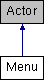
\includegraphics[height=2.000000cm]{class_menu}
\end{center}
\end{figure}
\subsection*{Public Member Functions}
\begin{DoxyCompactItemize}
\item 
\hyperlink{class_menu_a0c1481a62f6b0bf63a506d2622f2244f}{Menu} (void)
\begin{DoxyCompactList}\small\item\em Basic constructor. \end{DoxyCompactList}\item 
\hypertarget{class_menu_a73932d2ddab91e989102211f81c98c76}{\hyperlink{class_menu_a73932d2ddab91e989102211f81c98c76}{$\sim$\+Menu} (void)}\label{class_menu_a73932d2ddab91e989102211f81c98c76}

\begin{DoxyCompactList}\small\item\em Basic destructor. \end{DoxyCompactList}\item 
void \hyperlink{class_menu_a49984eb86ba63299629f3a84876499be}{show\+Menu} (\hyperlink{class_game}{Game} $\ast$game)
\begin{DoxyCompactList}\small\item\em The init menu function. \end{DoxyCompactList}\item 
void \hyperlink{class_menu_ab8cc125a548bd9d0c75ecc222df093e8}{Receive\+Message} (Message $\ast$m)
\begin{DoxyCompactList}\small\item\em Broadcast message function. \end{DoxyCompactList}\end{DoxyCompactItemize}


\subsection{Detailed Description}
Licensed to the Apache Software Foundation (A\+S\+F) under one or more contributor license agreements. See the N\+O\+T\+I\+C\+E file distributed with this work for additional information regarding copyright ownership. The A\+S\+F licenses this file to you under the Apache License, Version 2.\+0 (the \char`\"{}\+License\char`\"{}); you may not use this file except in compliance with the License. You may obtain a copy of the License at

\href{http://www.apache.org/licenses/LICENSE-2.0}{\tt http\+://www.\+apache.\+org/licenses/\+L\+I\+C\+E\+N\+S\+E-\/2.\+0}

Unless required by applicable law or agreed to in writing, software distributed under the License is distributed on an \char`\"{}\+A\+S I\+S\char`\"{} B\+A\+S\+I\+S, W\+I\+T\+H\+O\+U\+T W\+A\+R\+R\+A\+N\+T\+I\+E\+S O\+R C\+O\+N\+D\+I\+T\+I\+O\+N\+S O\+F A\+N\+Y K\+I\+N\+D, either express or implied. See the License for the specific language governing permissions and limitations under the License. File\+: \hyperlink{_menu_8hpp_source}{Menu.\+hpp} Creation\+: 2015-\/04-\/07 21\+:11 Louis Solofrizzo \href{mailto:louis@ne02ptzero.me}{\tt louis@ne02ptzero.\+me} 

\subsection{Constructor \& Destructor Documentation}
\hypertarget{class_menu_a0c1481a62f6b0bf63a506d2622f2244f}{\index{Menu@{Menu}!Menu@{Menu}}
\index{Menu@{Menu}!Menu@{Menu}}
\subsubsection[{Menu}]{\setlength{\rightskip}{0pt plus 5cm}Menu\+::\+Menu (
\begin{DoxyParamCaption}
\item[{void}]{}
\end{DoxyParamCaption}
)}}\label{class_menu_a0c1481a62f6b0bf63a506d2622f2244f}


Basic constructor. 

Licensed to the Apache Software Foundation (A\+S\+F) under one or more contributor license agreements. See the N\+O\+T\+I\+C\+E file distributed with this work for additional information regarding copyright ownership. The A\+S\+F licenses this file to you under the Apache License, Version 2.\+0 (the \char`\"{}\+License\char`\"{}); you may not use this file except in compliance with the License. You may obtain a copy of the License at

\href{http://www.apache.org/licenses/LICENSE-2.0}{\tt http\+://www.\+apache.\+org/licenses/\+L\+I\+C\+E\+N\+S\+E-\/2.\+0}

Unless required by applicable law or agreed to in writing, software distributed under the License is distributed on an \char`\"{}\+A\+S I\+S\char`\"{} B\+A\+S\+I\+S, W\+I\+T\+H\+O\+U\+T W\+A\+R\+R\+A\+N\+T\+I\+E\+S O\+R C\+O\+N\+D\+I\+T\+I\+O\+N\+S O\+F A\+N\+Y K\+I\+N\+D, either express or implied. See the License for the specific language governing permissions and limitations under the License. File\+: Menu.\+cpp Creation\+: 2015-\/04-\/07 21\+:11 Louis Solofrizzo \href{mailto:louis@ne02ptzero.me}{\tt louis@ne02ptzero.\+me} 

\subsection{Member Function Documentation}
\hypertarget{class_menu_ab8cc125a548bd9d0c75ecc222df093e8}{\index{Menu@{Menu}!Receive\+Message@{Receive\+Message}}
\index{Receive\+Message@{Receive\+Message}!Menu@{Menu}}
\subsubsection[{Receive\+Message}]{\setlength{\rightskip}{0pt plus 5cm}void Menu\+::\+Receive\+Message (
\begin{DoxyParamCaption}
\item[{Message $\ast$}]{m}
\end{DoxyParamCaption}
)}}\label{class_menu_ab8cc125a548bd9d0c75ecc222df093e8}


Broadcast message function. 

The intern Broadcast function. See Angel docs for more information 
\begin{DoxyParams}{Parameters}
{\em m} & The Message \hyperlink{class_object}{Object} \\
\hline
\end{DoxyParams}
\hypertarget{class_menu_a49984eb86ba63299629f3a84876499be}{\index{Menu@{Menu}!show\+Menu@{show\+Menu}}
\index{show\+Menu@{show\+Menu}!Menu@{Menu}}
\subsubsection[{show\+Menu}]{\setlength{\rightskip}{0pt plus 5cm}void Menu\+::show\+Menu (
\begin{DoxyParamCaption}
\item[{{\bf Game} $\ast$}]{game}
\end{DoxyParamCaption}
)}}\label{class_menu_a49984eb86ba63299629f3a84876499be}


The init menu function. 

Init the world, show the menu, and set the game for the future. 
\begin{DoxyParams}{Parameters}
{\em game} & The Main game class \\
\hline
\end{DoxyParams}
\begin{DoxySeeAlso}{See also}
\hyperlink{class_game}{Game} 
\end{DoxySeeAlso}


The documentation for this class was generated from the following files\+:\begin{DoxyCompactItemize}
\item 
inc/Menu.\+hpp\item 
src/Menu.\+cpp\end{DoxyCompactItemize}

\hypertarget{class_mouse_debugger}{\section{Mouse\-Debugger Class Reference}
\label{class_mouse_debugger}\index{Mouse\-Debugger@{Mouse\-Debugger}}
}


Inheritance diagram for Mouse\-Debugger\-:\nopagebreak
\begin{figure}[H]
\begin{center}
\leavevmode
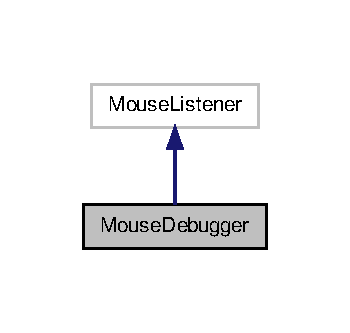
\includegraphics[width=168pt]{class_mouse_debugger__inherit__graph}
\end{center}
\end{figure}


Collaboration diagram for Mouse\-Debugger\-:\nopagebreak
\begin{figure}[H]
\begin{center}
\leavevmode
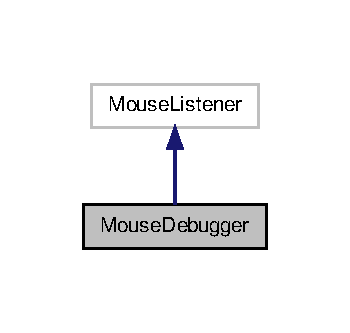
\includegraphics[width=168pt]{class_mouse_debugger__coll__graph}
\end{center}
\end{figure}
\subsection*{Public Member Functions}
\begin{DoxyCompactItemize}
\item 
\hyperlink{class_mouse_debugger_ad412f746c7415c334d346f40ba4c9a05}{Mouse\-Debugger} (void)
\item 
\hyperlink{class_mouse_debugger_a6b60c23ad59db3df59e3fefcacde9042}{$\sim$\-Mouse\-Debugger} (void)
\item 
void \hyperlink{class_mouse_debugger_a0d7f7e10a54cd1fc98370467805b24ac}{Mouse\-Down\-Event} (Vec2i sc, Mouse\-Button\-Input button)
\end{DoxyCompactItemize}


\subsection{Detailed Description}
Licensed to the Apache Software Foundation (A\-S\-F) under one or more contributor license agreements. See the N\-O\-T\-I\-C\-E file distributed with this work for additional information regarding copyright ownership. The A\-S\-F licenses this file to you under the Apache License, Version 2.\-0 (the \char`\"{}\-License\char`\"{}); you may not use this file except in compliance with the License. You may obtain a copy of the License at

\href{http://www.apache.org/licenses/LICENSE-2.0}{\tt http\-://www.\-apache.\-org/licenses/\-L\-I\-C\-E\-N\-S\-E-\/2.\-0}

Unless required by applicable law or agreed to in writing, software distributed under the License is distributed on an \char`\"{}\-A\-S I\-S\char`\"{} B\-A\-S\-I\-S, W\-I\-T\-H\-O\-U\-T W\-A\-R\-R\-A\-N\-T\-I\-E\-S O\-R C\-O\-N\-D\-I\-T\-I\-O\-N\-S O\-F A\-N\-Y K\-I\-N\-D, either express or implied. See the License for the specific language governing permissions and limitations under the License. File\-: \hyperlink{main_8cpp}{main.\-cpp} Creation\-: 2015-\/02-\/13 10\-:30 Louis Solofrizzo \href{mailto:louis@ne02ptzero.me}{\tt louis@ne02ptzero.\-me} 

\subsection{Constructor \& Destructor Documentation}
\hypertarget{class_mouse_debugger_ad412f746c7415c334d346f40ba4c9a05}{\index{Mouse\-Debugger@{Mouse\-Debugger}!Mouse\-Debugger@{Mouse\-Debugger}}
\index{Mouse\-Debugger@{Mouse\-Debugger}!MouseDebugger@{Mouse\-Debugger}}
\subsubsection[{Mouse\-Debugger}]{\setlength{\rightskip}{0pt plus 5cm}Mouse\-Debugger\-::\-Mouse\-Debugger (
\begin{DoxyParamCaption}
\item[{void}]{}
\end{DoxyParamCaption}
)\hspace{0.3cm}{\ttfamily [inline]}}}\label{class_mouse_debugger_ad412f746c7415c334d346f40ba4c9a05}
\hypertarget{class_mouse_debugger_a6b60c23ad59db3df59e3fefcacde9042}{\index{Mouse\-Debugger@{Mouse\-Debugger}!$\sim$\-Mouse\-Debugger@{$\sim$\-Mouse\-Debugger}}
\index{$\sim$\-Mouse\-Debugger@{$\sim$\-Mouse\-Debugger}!MouseDebugger@{Mouse\-Debugger}}
\subsubsection[{$\sim$\-Mouse\-Debugger}]{\setlength{\rightskip}{0pt plus 5cm}Mouse\-Debugger\-::$\sim$\-Mouse\-Debugger (
\begin{DoxyParamCaption}
\item[{void}]{}
\end{DoxyParamCaption}
)\hspace{0.3cm}{\ttfamily [inline]}}}\label{class_mouse_debugger_a6b60c23ad59db3df59e3fefcacde9042}


\subsection{Member Function Documentation}
\hypertarget{class_mouse_debugger_a0d7f7e10a54cd1fc98370467805b24ac}{\index{Mouse\-Debugger@{Mouse\-Debugger}!Mouse\-Down\-Event@{Mouse\-Down\-Event}}
\index{Mouse\-Down\-Event@{Mouse\-Down\-Event}!MouseDebugger@{Mouse\-Debugger}}
\subsubsection[{Mouse\-Down\-Event}]{\setlength{\rightskip}{0pt plus 5cm}void Mouse\-Debugger\-::\-Mouse\-Down\-Event (
\begin{DoxyParamCaption}
\item[{Vec2i}]{sc, }
\item[{Mouse\-Button\-Input}]{button}
\end{DoxyParamCaption}
)\hspace{0.3cm}{\ttfamily [inline]}}}\label{class_mouse_debugger_a0d7f7e10a54cd1fc98370467805b24ac}


The documentation for this class was generated from the following file\-:\begin{DoxyCompactItemize}
\item 
/home/louis/\-Documents/rogue-\/like/\-Sources/src/\hyperlink{main_8cpp}{main.\-cpp}\end{DoxyCompactItemize}

\hypertarget{class_object}{\section{Object Class Reference}
\label{class_object}\index{Object@{Object}}
}


{\ttfamily \#include $<$Object.\+hpp$>$}

Inheritance diagram for Object\+:\begin{figure}[H]
\begin{center}
\leavevmode
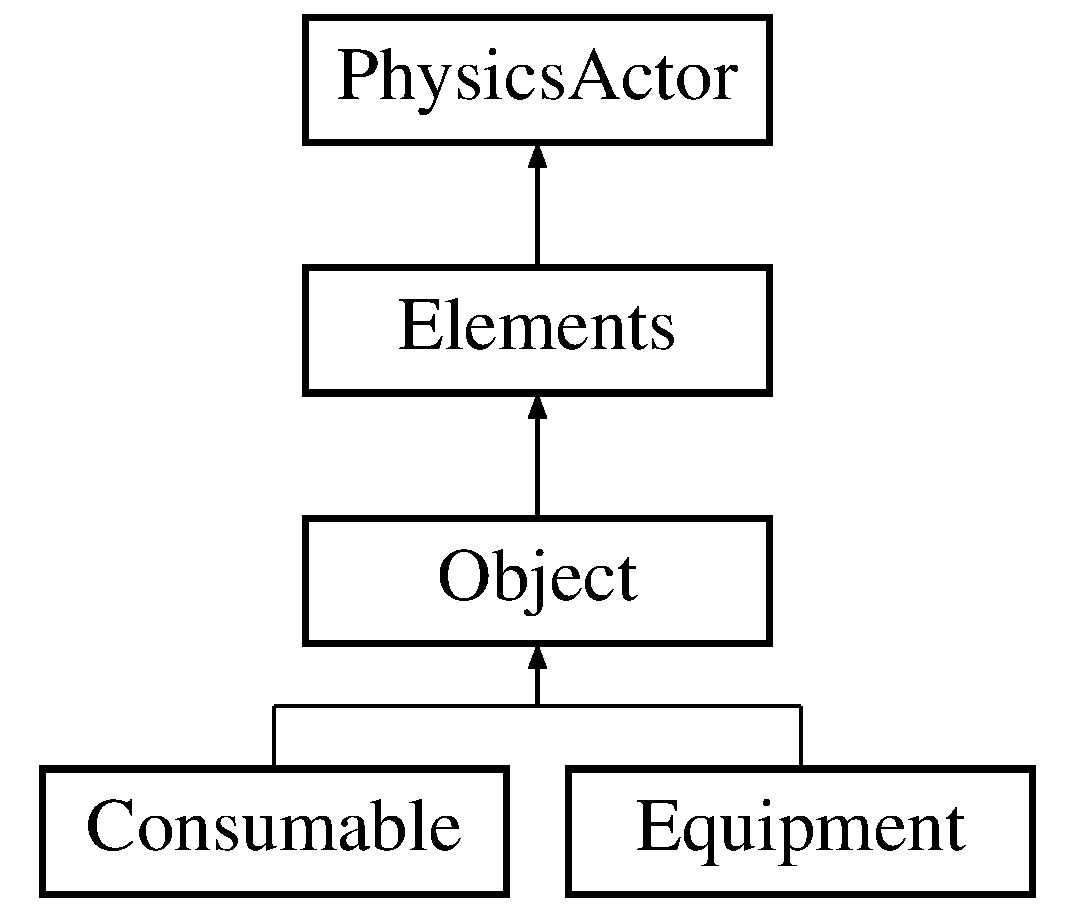
\includegraphics[height=4.000000cm]{class_object}
\end{center}
\end{figure}
\subsection*{Public Member Functions}
\begin{DoxyCompactItemize}
\item 
\hyperlink{class_object_a40860402e64d8008fb42329df7097cdb}{Object} ()
\begin{DoxyCompactList}\small\item\em Constructor. \end{DoxyCompactList}\item 
\hyperlink{class_object_ae8f5483f459e46687bd01e6f9977afd3}{$\sim$\+Object} ()
\begin{DoxyCompactList}\small\item\em Destructor. \end{DoxyCompactList}\item 
void \hyperlink{class_object_a5681745b50d64994e00fe519bbb4cd31}{Begin\+Contact} (\hyperlink{class_elements}{Elements} $\ast$elem, b2\+Contact $\ast$contact)
\begin{DoxyCompactList}\small\item\em Overload from b2\+Body's Begin\+Contact. \end{DoxyCompactList}\end{DoxyCompactItemize}
\subsection*{Additional Inherited Members}


\subsection{Detailed Description}
Licensed to the Apache Software Foundation (A\+S\+F) under one or more contributor license agreements. See the N\+O\+T\+I\+C\+E file distributed with this work for additional information regarding copyright ownership. The A\+S\+F licenses this file to you under the Apache License, Version 2.\+0 (the \char`\"{}\+License\char`\"{}); you may not use this file except in compliance with the License. You may obtain a copy of the License at

\href{http://www.apache.org/licenses/LICENSE-2.0}{\tt http\+://www.\+apache.\+org/licenses/\+L\+I\+C\+E\+N\+S\+E-\/2.\+0}

Unless required by applicable law or agreed to in writing, software distributed under the License is distributed on an \char`\"{}\+A\+S I\+S\char`\"{} B\+A\+S\+I\+S, W\+I\+T\+H\+O\+U\+T W\+A\+R\+R\+A\+N\+T\+I\+E\+S O\+R C\+O\+N\+D\+I\+T\+I\+O\+N\+S O\+F A\+N\+Y K\+I\+N\+D, either express or implied. See the License for the specific language governing permissions and limitations under the License. File\+: \hyperlink{_object_8hpp_source}{Object.\+hpp} Creation\+: 2015-\/03-\/03 13\+:10 Manon Budin \href{mailto:mbudin@student.42.fr}{\tt mbudin@student.\+42.\+fr} 

\subsection{Constructor \& Destructor Documentation}
\hypertarget{class_object_a40860402e64d8008fb42329df7097cdb}{\index{Object@{Object}!Object@{Object}}
\index{Object@{Object}!Object@{Object}}
\subsubsection[{Object}]{\setlength{\rightskip}{0pt plus 5cm}Object\+::\+Object (
\begin{DoxyParamCaption}
\item[{void}]{}
\end{DoxyParamCaption}
)}}\label{class_object_a40860402e64d8008fb42329df7097cdb}


Constructor. 

Licensed to the Apache Software Foundation (A\+S\+F) under one or more contributor license agreements. See the N\+O\+T\+I\+C\+E file distributed with this work for additional information regarding copyright ownership. The A\+S\+F licenses this file to you under the Apache License, Version 2.\+0 (the \char`\"{}\+License\char`\"{}); you may not use this file except in compliance with the License. You may obtain a copy of the License at

\href{http://www.apache.org/licenses/LICENSE-2.0}{\tt http\+://www.\+apache.\+org/licenses/\+L\+I\+C\+E\+N\+S\+E-\/2.\+0}

Unless required by applicable law or agreed to in writing, software distributed under the License is distributed on an \char`\"{}\+A\+S I\+S\char`\"{} B\+A\+S\+I\+S, W\+I\+T\+H\+O\+U\+T W\+A\+R\+R\+A\+N\+T\+I\+E\+S O\+R C\+O\+N\+D\+I\+T\+I\+O\+N\+S O\+F A\+N\+Y K\+I\+N\+D, either express or implied. See the License for the specific language governing permissions and limitations under the License. File\+: Object.\+cpp Creation\+: 2015-\/03-\/03 13\+:08 Manon Budin \href{mailto:mbudin@student.42.fr}{\tt mbudin@student.\+42.\+fr} Basic Constructor \hypertarget{class_object_ae8f5483f459e46687bd01e6f9977afd3}{\index{Object@{Object}!````~Object@{$\sim$\+Object}}
\index{````~Object@{$\sim$\+Object}!Object@{Object}}
\subsubsection[{$\sim$\+Object}]{\setlength{\rightskip}{0pt plus 5cm}Object\+::$\sim$\+Object (
\begin{DoxyParamCaption}
\item[{void}]{}
\end{DoxyParamCaption}
)}}\label{class_object_ae8f5483f459e46687bd01e6f9977afd3}


Destructor. 

Basic Destructor 

\subsection{Member Function Documentation}
\hypertarget{class_object_a5681745b50d64994e00fe519bbb4cd31}{\index{Object@{Object}!Begin\+Contact@{Begin\+Contact}}
\index{Begin\+Contact@{Begin\+Contact}!Object@{Object}}
\subsubsection[{Begin\+Contact}]{\setlength{\rightskip}{0pt plus 5cm}void Object\+::\+Begin\+Contact (
\begin{DoxyParamCaption}
\item[{{\bf Elements} $\ast$}]{elem, }
\item[{b2\+Contact $\ast$}]{contact}
\end{DoxyParamCaption}
)\hspace{0.3cm}{\ttfamily [virtual]}}}\label{class_object_a5681745b50d64994e00fe519bbb4cd31}


Overload from b2\+Body's Begin\+Contact. 

Collision begin callback 
\begin{DoxyParams}{Parameters}
{\em elem} & (\hyperlink{class_elements}{Elements} $\ast$) \\
\hline
{\em contact} & (b2\+Contact $\ast$) \\
\hline
\end{DoxyParams}
\begin{DoxyNote}{Note}
This function is called just before a collision 
\end{DoxyNote}


Reimplemented from \hyperlink{class_elements}{Elements}.



The documentation for this class was generated from the following files\+:\begin{DoxyCompactItemize}
\item 
inc/Object.\+hpp\item 
src/Object.\+cpp\end{DoxyCompactItemize}

\hypertarget{class_projectile}{\section{Projectile Class Reference}
\label{class_projectile}\index{Projectile@{Projectile}}
}
Inheritance diagram for Projectile\+:\begin{figure}[H]
\begin{center}
\leavevmode
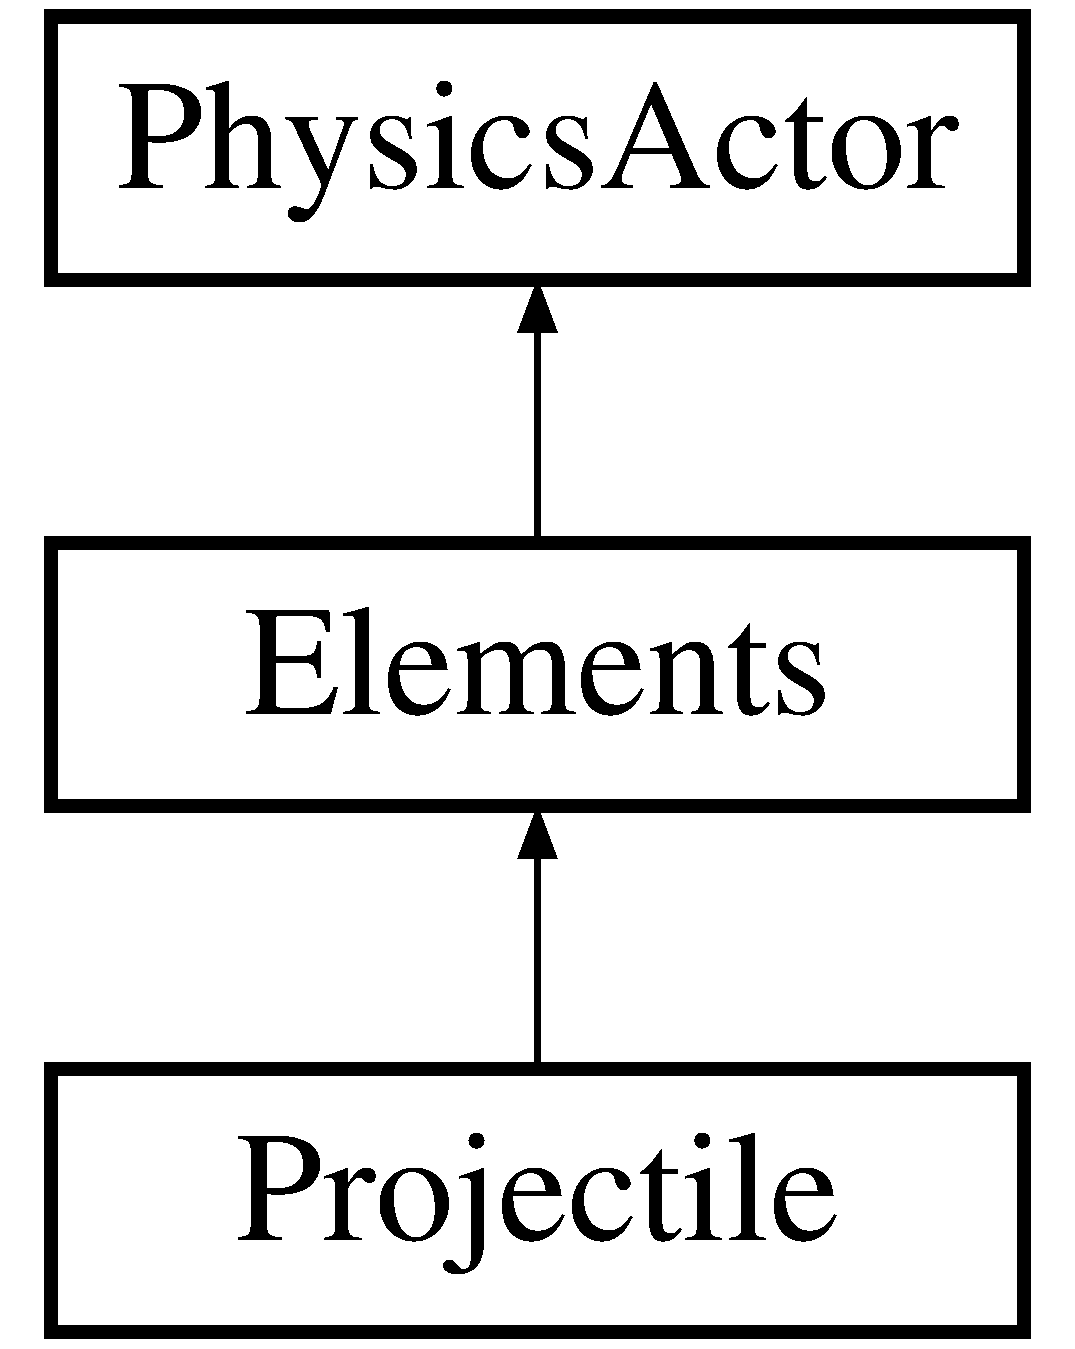
\includegraphics[height=3.000000cm]{class_projectile}
\end{center}
\end{figure}
\subsection*{Public Member Functions}
\begin{DoxyCompactItemize}
\item 
\hypertarget{class_projectile_aa77304b2b631673899c673ea5ff660bd}{{\bfseries Projectile} (float x, float y, int direction, std\+::string owner)}\label{class_projectile_aa77304b2b631673899c673ea5ff660bd}

\item 
\hyperlink{class_projectile_a2131209b192886d9be4fcabe3511a1d3}{Projectile} (\hyperlink{class_weapon}{Weapon} $\ast$w, \hyperlink{class_characters}{Characters} $\ast$c)
\begin{DoxyCompactList}\small\item\em Constructor called by the \hyperlink{class_weapon}{Weapon} class, when an attack was ordered using a ranged weapon. \end{DoxyCompactList}\item 
\hypertarget{class_projectile_ace3baa31fb47d65321b3091e55ea0214}{std\+::string {\bfseries get\+Name} (void)}\label{class_projectile_ace3baa31fb47d65321b3091e55ea0214}

\item 
\hypertarget{class_projectile_a259c762588761610eb08f4590409be47}{std\+::string {\bfseries get\+Flavor} (void)}\label{class_projectile_a259c762588761610eb08f4590409be47}

\item 
\hypertarget{class_projectile_a3d296e98b7227371fdfcfd9fef8bf505}{std\+::string {\bfseries get\+Attack} (void)}\label{class_projectile_a3d296e98b7227371fdfcfd9fef8bf505}

\item 
\hypertarget{class_projectile_a2342bda48bea3511d0b97f5cba7b095f}{float {\bfseries get\+Active} (void)}\label{class_projectile_a2342bda48bea3511d0b97f5cba7b095f}

\item 
\hypertarget{class_projectile_a284ae1c52821f8a9bd5972793eb210d8}{int {\bfseries get\+Size} (void)}\label{class_projectile_a284ae1c52821f8a9bd5972793eb210d8}

\item 
\hypertarget{class_projectile_ab86af40b130ac18871e9a4baec80dc85}{int {\bfseries get\+Damage} (void)}\label{class_projectile_ab86af40b130ac18871e9a4baec80dc85}

\item 
\hypertarget{class_projectile_ad54c17a658890109a332e643bb8446f2}{int {\bfseries get\+Pushback} (void)}\label{class_projectile_ad54c17a658890109a332e643bb8446f2}

\item 
\hypertarget{class_projectile_acf9cf10cbb254d444c9b617bd0baf075}{float {\bfseries get\+Recovery} (void)}\label{class_projectile_acf9cf10cbb254d444c9b617bd0baf075}

\item 
\hypertarget{class_projectile_acdc9aa548f9606221bb3fe15e4a7dfa7}{int {\bfseries attack\+Ready} (void)}\label{class_projectile_acdc9aa548f9606221bb3fe15e4a7dfa7}

\item 
void \hyperlink{class_projectile_a7347375e9c8cae921709ba56265af0fd}{Begin\+Contact} (\hyperlink{class_elements}{Elements} $\ast$elem, b2\+Contact $\ast$contact)
\begin{DoxyCompactList}\small\item\em Overload from b2\+Body's Begin\+Contact. \end{DoxyCompactList}\item 
\hypertarget{class_projectile_a9f8fa9403a414fa1fd6ee092720ca4e6}{void {\bfseries End\+Contact} (\hyperlink{class_elements}{Elements} $\ast$elem, b2\+Contact $\ast$contact)}\label{class_projectile_a9f8fa9403a414fa1fd6ee092720ca4e6}

\item 
\hypertarget{class_projectile_aa5247586a6ca84625abed35767b8f282}{void {\bfseries Receive\+Message} (Message $\ast$m)}\label{class_projectile_aa5247586a6ca84625abed35767b8f282}

\end{DoxyCompactItemize}
\subsection*{Additional Inherited Members}


\subsection{Constructor \& Destructor Documentation}
\hypertarget{class_projectile_a2131209b192886d9be4fcabe3511a1d3}{\index{Projectile@{Projectile}!Projectile@{Projectile}}
\index{Projectile@{Projectile}!Projectile@{Projectile}}
\subsubsection[{Projectile}]{\setlength{\rightskip}{0pt plus 5cm}Projectile\+::\+Projectile (
\begin{DoxyParamCaption}
\item[{{\bf Weapon} $\ast$}]{w, }
\item[{{\bf Characters} $\ast$}]{c}
\end{DoxyParamCaption}
)}}\label{class_projectile_a2131209b192886d9be4fcabe3511a1d3}


Constructor called by the \hyperlink{class_weapon}{Weapon} class, when an attack was ordered using a ranged weapon. 

Licensed to the Apache Software Foundation (A\+S\+F) under one or more contributor license agreements. See the N\+O\+T\+I\+C\+E file distributed with this work for additional information regarding copyright ownership. The A\+S\+F licenses this file to you under the Apache License, Version 2.\+0 (the \char`\"{}\+License\char`\"{}); you may not use this file except in compliance with the License. You may obtain a copy of the License at

\href{http://www.apache.org/licenses/LICENSE-2.0}{\tt http\+://www.\+apache.\+org/licenses/\+L\+I\+C\+E\+N\+S\+E-\/2.\+0}

Unless required by applicable law or agreed to in writing, software distributed under the License is distributed on an \char`\"{}\+A\+S I\+S\char`\"{} B\+A\+S\+I\+S, W\+I\+T\+H\+O\+U\+T W\+A\+R\+R\+A\+N\+T\+I\+E\+S O\+R C\+O\+N\+D\+I\+T\+I\+O\+N\+S O\+F A\+N\+Y K\+I\+N\+D, either express or implied. See the License for the specific language governing permissions and limitations under the License. File\+: Projectile.\+cpp Creation\+: 2015-\/02-\/23 15\+:140 Matthieu Maudet \href{mailto:mmaudet@student.42.fr}{\tt mmaudet@student.\+42.\+fr} Default constructor 
\begin{DoxyParams}{Parameters}
{\em w} & Weapon$\ast$ (weapon object which called the attack) \\
\hline
{\em c} & Characters$\ast$ (\hyperlink{class_characters}{Characters} object which currently carries the weapon) \\
\hline
\end{DoxyParams}


\subsection{Member Function Documentation}
\hypertarget{class_projectile_a7347375e9c8cae921709ba56265af0fd}{\index{Projectile@{Projectile}!Begin\+Contact@{Begin\+Contact}}
\index{Begin\+Contact@{Begin\+Contact}!Projectile@{Projectile}}
\subsubsection[{Begin\+Contact}]{\setlength{\rightskip}{0pt plus 5cm}void Projectile\+::\+Begin\+Contact (
\begin{DoxyParamCaption}
\item[{{\bf Elements} $\ast$}]{m, }
\item[{b2\+Contact $\ast$}]{c}
\end{DoxyParamCaption}
)\hspace{0.3cm}{\ttfamily [virtual]}}}\label{class_projectile_a7347375e9c8cae921709ba56265af0fd}


Overload from b2\+Body's Begin\+Contact. 

Collision begin callback See Angel docs for more information. /!\textbackslash{} This function is called B\+E\+F\+O\+R\+E a collision happened. 
\begin{DoxyParams}{Parameters}
{\em elem} & The Element who collide \\
\hline
{\em contact} & The b2\+Contact object of the collision. See Box2\+D docs for more info. \\
\hline
\end{DoxyParams}


Reimplemented from \hyperlink{class_elements}{Elements}.



The documentation for this class was generated from the following files\+:\begin{DoxyCompactItemize}
\item 
Sources/inc/Projectile.\+hpp\item 
Sources/src/Projectile.\+cpp\end{DoxyCompactItemize}

\hypertarget{class_room}{\section{Room Class Reference}
\label{class_room}\index{Room@{Room}}
}


{\ttfamily \#include $<$Room.\-hpp$>$}

\subsection*{Public Member Functions}
\begin{DoxyCompactItemize}
\item 
\hyperlink{class_room_aaef0b08fe3796290d4609470ddd9a0c4}{Room} (int id, int \hyperlink{jquery_8js_a4c3eadaa5164016d2c340d495fc6e55e}{x}, int y, int map\-Id)
\item 
\hyperlink{class_room_a67d5da09983cc53097807fd43ba5481a}{$\sim$\-Room} ()
\item 
int \hyperlink{class_room_a067f0dbf1e1981f3f53692c454032bad}{get\-X} () const 
\item 
int \hyperlink{class_room_a36707f281040aa8d27f13070b1a35b20}{get\-Y} () const 
\item 
int \hyperlink{class_room_ad36e96122696a31eec31a52ac99c4a4b}{get\-Map\-Id} () const 
\item 
int \hyperlink{class_room_a6f71af918166e1835662982219559d29}{get\-Id} () const 
\item 
int \hyperlink{class_room_a977bd80b8c374edb31eb467d191b7233}{get\-Distance} () const 
\item 
int \hyperlink{class_room_a63e8fe415cd7f3e7f327bf7603388638}{get\-Links} () const 
\item 
\hyperlink{_room_8hpp_a3879bd0aba9f20985139f480b9f73323}{Special\-Type} \hyperlink{class_room_a97488664cbabc4cef3a63d18526b5fc0}{get\-Special\-Type} () const 
\item 
bool \hyperlink{class_room_ad490b94e5406c002c875b4a507674008}{get\-Top\-Door} () const 
\item 
bool \hyperlink{class_room_a3b86ce135752e252c7f2900f29abbb6f}{get\-Left\-Door} () const 
\item 
bool \hyperlink{class_room_acb8b99c54a262c532a2b4f388fafc36a}{get\-Bottom\-Door} () const 
\item 
bool \hyperlink{class_room_a257c82e3ac31634b8612c33900fc28bc}{get\-Right\-Door} () const 
\item 
void \hyperlink{class_room_ab9ce2180afaa86a1881a245d1b539e03}{add\-Link} ()
\item 
void \hyperlink{class_room_a6918ec80b6c291bbce3a9f8d8889222f}{set\-Top\-Door} (bool state)
\item 
void \hyperlink{class_room_afe6694b78ba1754048dcba4e6036c9a5}{set\-Left\-Door} (bool state)
\item 
void \hyperlink{class_room_a6bd75cbe373514583b67b6131e484814}{set\-Bottom\-Door} (bool state)
\item 
void \hyperlink{class_room_a5ba5a9b9807f26d2ea17c8b9377214af}{set\-Right\-Door} (bool state)
\item 
void \hyperlink{class_room_a8515625370a9aec953f76efded718e4b}{set\-Distance} (int distance)
\item 
void \hyperlink{class_room_a5c58b28fceef732f7cf3f865209ab847}{set\-Special\-Type} (\hyperlink{_room_8hpp_a3879bd0aba9f20985139f480b9f73323}{Special\-Type} type)
\end{DoxyCompactItemize}


\subsection{Constructor \& Destructor Documentation}
\hypertarget{class_room_aaef0b08fe3796290d4609470ddd9a0c4}{\index{Room@{Room}!Room@{Room}}
\index{Room@{Room}!Room@{Room}}
\subsubsection[{Room}]{\setlength{\rightskip}{0pt plus 5cm}Room\-::\-Room (
\begin{DoxyParamCaption}
\item[{int}]{id, }
\item[{int}]{y, }
\item[{int}]{x, }
\item[{int}]{map\-Id}
\end{DoxyParamCaption}
)}}\label{class_room_aaef0b08fe3796290d4609470ddd9a0c4}
Licensed to the Apache Software Foundation (A\-S\-F) under one or more contributor license agreements. See the N\-O\-T\-I\-C\-E file distributed with this work for additional information regarding copyright ownership. The A\-S\-F licenses this file to you under the Apache License, Version 2.\-0 (the \char`\"{}\-License\char`\"{}); you may not use this file except in compliance with the License. You may obtain a copy of the License at

\href{http://www.apache.org/licenses/LICENSE-2.0}{\tt http\-://www.\-apache.\-org/licenses/\-L\-I\-C\-E\-N\-S\-E-\/2.\-0}

Unless required by applicable law or agreed to in writing, software distributed under the License is distributed on an \char`\"{}\-A\-S I\-S\char`\"{} B\-A\-S\-I\-S, W\-I\-T\-H\-O\-U\-T W\-A\-R\-R\-A\-N\-T\-I\-E\-S O\-R C\-O\-N\-D\-I\-T\-I\-O\-N\-S O\-F A\-N\-Y K\-I\-N\-D, either express or implied. See the License for the specific language governing permissions and limitations under the License. File\-: \hyperlink{_level_generator_8cpp}{Level\-Generator.\-cpp} Creation\-: 2015-\/03-\/02 16\-:05 Matthieu Maudet \href{mailto:mmaudet@student.42.fr}{\tt mmaudet@student.\-42.\-fr} Basic constructor \hypertarget{class_room_a67d5da09983cc53097807fd43ba5481a}{\index{Room@{Room}!$\sim$\-Room@{$\sim$\-Room}}
\index{$\sim$\-Room@{$\sim$\-Room}!Room@{Room}}
\subsubsection[{$\sim$\-Room}]{\setlength{\rightskip}{0pt plus 5cm}Room\-::$\sim$\-Room (
\begin{DoxyParamCaption}
\item[{void}]{}
\end{DoxyParamCaption}
)}}\label{class_room_a67d5da09983cc53097807fd43ba5481a}
Basic Destructor 

\subsection{Member Function Documentation}
\hypertarget{class_room_ab9ce2180afaa86a1881a245d1b539e03}{\index{Room@{Room}!add\-Link@{add\-Link}}
\index{add\-Link@{add\-Link}!Room@{Room}}
\subsubsection[{add\-Link}]{\setlength{\rightskip}{0pt plus 5cm}void Room\-::add\-Link (
\begin{DoxyParamCaption}
\item[{void}]{}
\end{DoxyParamCaption}
)}}\label{class_room_ab9ce2180afaa86a1881a245d1b539e03}
\hypertarget{class_room_acb8b99c54a262c532a2b4f388fafc36a}{\index{Room@{Room}!get\-Bottom\-Door@{get\-Bottom\-Door}}
\index{get\-Bottom\-Door@{get\-Bottom\-Door}!Room@{Room}}
\subsubsection[{get\-Bottom\-Door}]{\setlength{\rightskip}{0pt plus 5cm}bool Room\-::get\-Bottom\-Door (
\begin{DoxyParamCaption}
\item[{void}]{}
\end{DoxyParamCaption}
) const}}\label{class_room_acb8b99c54a262c532a2b4f388fafc36a}
\hypertarget{class_room_a977bd80b8c374edb31eb467d191b7233}{\index{Room@{Room}!get\-Distance@{get\-Distance}}
\index{get\-Distance@{get\-Distance}!Room@{Room}}
\subsubsection[{get\-Distance}]{\setlength{\rightskip}{0pt plus 5cm}int Room\-::get\-Distance (
\begin{DoxyParamCaption}
\item[{void}]{}
\end{DoxyParamCaption}
) const}}\label{class_room_a977bd80b8c374edb31eb467d191b7233}
\hypertarget{class_room_a6f71af918166e1835662982219559d29}{\index{Room@{Room}!get\-Id@{get\-Id}}
\index{get\-Id@{get\-Id}!Room@{Room}}
\subsubsection[{get\-Id}]{\setlength{\rightskip}{0pt plus 5cm}int Room\-::get\-Id (
\begin{DoxyParamCaption}
\item[{void}]{}
\end{DoxyParamCaption}
) const}}\label{class_room_a6f71af918166e1835662982219559d29}
\hypertarget{class_room_a3b86ce135752e252c7f2900f29abbb6f}{\index{Room@{Room}!get\-Left\-Door@{get\-Left\-Door}}
\index{get\-Left\-Door@{get\-Left\-Door}!Room@{Room}}
\subsubsection[{get\-Left\-Door}]{\setlength{\rightskip}{0pt plus 5cm}bool Room\-::get\-Left\-Door (
\begin{DoxyParamCaption}
\item[{void}]{}
\end{DoxyParamCaption}
) const}}\label{class_room_a3b86ce135752e252c7f2900f29abbb6f}
\hypertarget{class_room_a63e8fe415cd7f3e7f327bf7603388638}{\index{Room@{Room}!get\-Links@{get\-Links}}
\index{get\-Links@{get\-Links}!Room@{Room}}
\subsubsection[{get\-Links}]{\setlength{\rightskip}{0pt plus 5cm}int Room\-::get\-Links (
\begin{DoxyParamCaption}
\item[{void}]{}
\end{DoxyParamCaption}
) const}}\label{class_room_a63e8fe415cd7f3e7f327bf7603388638}
\hypertarget{class_room_ad36e96122696a31eec31a52ac99c4a4b}{\index{Room@{Room}!get\-Map\-Id@{get\-Map\-Id}}
\index{get\-Map\-Id@{get\-Map\-Id}!Room@{Room}}
\subsubsection[{get\-Map\-Id}]{\setlength{\rightskip}{0pt plus 5cm}int Room\-::get\-Map\-Id (
\begin{DoxyParamCaption}
\item[{void}]{}
\end{DoxyParamCaption}
) const}}\label{class_room_ad36e96122696a31eec31a52ac99c4a4b}
\hypertarget{class_room_a257c82e3ac31634b8612c33900fc28bc}{\index{Room@{Room}!get\-Right\-Door@{get\-Right\-Door}}
\index{get\-Right\-Door@{get\-Right\-Door}!Room@{Room}}
\subsubsection[{get\-Right\-Door}]{\setlength{\rightskip}{0pt plus 5cm}bool Room\-::get\-Right\-Door (
\begin{DoxyParamCaption}
\item[{void}]{}
\end{DoxyParamCaption}
) const}}\label{class_room_a257c82e3ac31634b8612c33900fc28bc}
\hypertarget{class_room_a97488664cbabc4cef3a63d18526b5fc0}{\index{Room@{Room}!get\-Special\-Type@{get\-Special\-Type}}
\index{get\-Special\-Type@{get\-Special\-Type}!Room@{Room}}
\subsubsection[{get\-Special\-Type}]{\setlength{\rightskip}{0pt plus 5cm}{\bf Special\-Type} Room\-::get\-Special\-Type (
\begin{DoxyParamCaption}
\item[{void}]{}
\end{DoxyParamCaption}
) const}}\label{class_room_a97488664cbabc4cef3a63d18526b5fc0}
\hypertarget{class_room_ad490b94e5406c002c875b4a507674008}{\index{Room@{Room}!get\-Top\-Door@{get\-Top\-Door}}
\index{get\-Top\-Door@{get\-Top\-Door}!Room@{Room}}
\subsubsection[{get\-Top\-Door}]{\setlength{\rightskip}{0pt plus 5cm}bool Room\-::get\-Top\-Door (
\begin{DoxyParamCaption}
\item[{void}]{}
\end{DoxyParamCaption}
) const}}\label{class_room_ad490b94e5406c002c875b4a507674008}
\hypertarget{class_room_a067f0dbf1e1981f3f53692c454032bad}{\index{Room@{Room}!get\-X@{get\-X}}
\index{get\-X@{get\-X}!Room@{Room}}
\subsubsection[{get\-X}]{\setlength{\rightskip}{0pt plus 5cm}int Room\-::get\-X (
\begin{DoxyParamCaption}
\item[{void}]{}
\end{DoxyParamCaption}
) const}}\label{class_room_a067f0dbf1e1981f3f53692c454032bad}
\hypertarget{class_room_a36707f281040aa8d27f13070b1a35b20}{\index{Room@{Room}!get\-Y@{get\-Y}}
\index{get\-Y@{get\-Y}!Room@{Room}}
\subsubsection[{get\-Y}]{\setlength{\rightskip}{0pt plus 5cm}int Room\-::get\-Y (
\begin{DoxyParamCaption}
\item[{void}]{}
\end{DoxyParamCaption}
) const}}\label{class_room_a36707f281040aa8d27f13070b1a35b20}
\hypertarget{class_room_a6bd75cbe373514583b67b6131e484814}{\index{Room@{Room}!set\-Bottom\-Door@{set\-Bottom\-Door}}
\index{set\-Bottom\-Door@{set\-Bottom\-Door}!Room@{Room}}
\subsubsection[{set\-Bottom\-Door}]{\setlength{\rightskip}{0pt plus 5cm}void Room\-::set\-Bottom\-Door (
\begin{DoxyParamCaption}
\item[{bool}]{state}
\end{DoxyParamCaption}
)}}\label{class_room_a6bd75cbe373514583b67b6131e484814}
\hypertarget{class_room_a8515625370a9aec953f76efded718e4b}{\index{Room@{Room}!set\-Distance@{set\-Distance}}
\index{set\-Distance@{set\-Distance}!Room@{Room}}
\subsubsection[{set\-Distance}]{\setlength{\rightskip}{0pt plus 5cm}void Room\-::set\-Distance (
\begin{DoxyParamCaption}
\item[{int}]{distance}
\end{DoxyParamCaption}
)}}\label{class_room_a8515625370a9aec953f76efded718e4b}
\hypertarget{class_room_afe6694b78ba1754048dcba4e6036c9a5}{\index{Room@{Room}!set\-Left\-Door@{set\-Left\-Door}}
\index{set\-Left\-Door@{set\-Left\-Door}!Room@{Room}}
\subsubsection[{set\-Left\-Door}]{\setlength{\rightskip}{0pt plus 5cm}void Room\-::set\-Left\-Door (
\begin{DoxyParamCaption}
\item[{bool}]{state}
\end{DoxyParamCaption}
)}}\label{class_room_afe6694b78ba1754048dcba4e6036c9a5}
\hypertarget{class_room_a5ba5a9b9807f26d2ea17c8b9377214af}{\index{Room@{Room}!set\-Right\-Door@{set\-Right\-Door}}
\index{set\-Right\-Door@{set\-Right\-Door}!Room@{Room}}
\subsubsection[{set\-Right\-Door}]{\setlength{\rightskip}{0pt plus 5cm}void Room\-::set\-Right\-Door (
\begin{DoxyParamCaption}
\item[{bool}]{state}
\end{DoxyParamCaption}
)}}\label{class_room_a5ba5a9b9807f26d2ea17c8b9377214af}
\hypertarget{class_room_a5c58b28fceef732f7cf3f865209ab847}{\index{Room@{Room}!set\-Special\-Type@{set\-Special\-Type}}
\index{set\-Special\-Type@{set\-Special\-Type}!Room@{Room}}
\subsubsection[{set\-Special\-Type}]{\setlength{\rightskip}{0pt plus 5cm}void Room\-::set\-Special\-Type (
\begin{DoxyParamCaption}
\item[{{\bf Special\-Type}}]{type}
\end{DoxyParamCaption}
)}}\label{class_room_a5c58b28fceef732f7cf3f865209ab847}
\hypertarget{class_room_a6918ec80b6c291bbce3a9f8d8889222f}{\index{Room@{Room}!set\-Top\-Door@{set\-Top\-Door}}
\index{set\-Top\-Door@{set\-Top\-Door}!Room@{Room}}
\subsubsection[{set\-Top\-Door}]{\setlength{\rightskip}{0pt plus 5cm}void Room\-::set\-Top\-Door (
\begin{DoxyParamCaption}
\item[{bool}]{state}
\end{DoxyParamCaption}
)}}\label{class_room_a6918ec80b6c291bbce3a9f8d8889222f}


The documentation for this class was generated from the following files\-:\begin{DoxyCompactItemize}
\item 
/home/louis/\-Documents/rogue-\/like/\-Sources/inc/\hyperlink{_room_8hpp}{Room.\-hpp}\item 
/home/louis/\-Documents/rogue-\/like/\-Sources/src/\hyperlink{_room_8cpp}{Room.\-cpp}\end{DoxyCompactItemize}

\hypertarget{class_shooter}{\section{Shooter Class Reference}
\label{class_shooter}\index{Shooter@{Shooter}}
}


{\ttfamily \#include $<$Shooter.\-hpp$>$}



Inheritance diagram for Shooter\-:\nopagebreak
\begin{figure}[H]
\begin{center}
\leavevmode
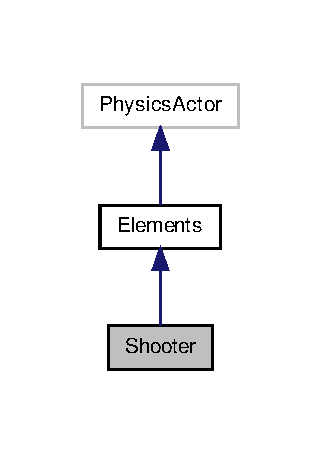
\includegraphics[width=154pt]{class_shooter__inherit__graph}
\end{center}
\end{figure}


Collaboration diagram for Shooter\-:\nopagebreak
\begin{figure}[H]
\begin{center}
\leavevmode
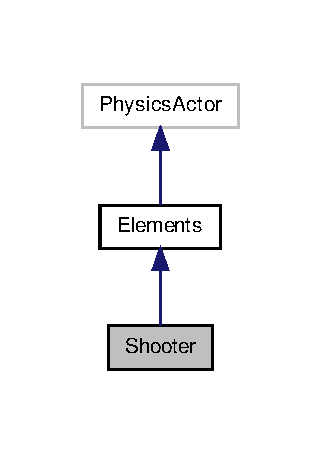
\includegraphics[width=154pt]{class_shooter__coll__graph}
\end{center}
\end{figure}
\subsection*{Public Member Functions}
\begin{DoxyCompactItemize}
\item 
\hyperlink{class_shooter_acc429ebafcc36bb592c752097c22657f}{Shooter} ()
\item 
\hypertarget{class_shooter_adc34229494950169d09804f1d524ac7d}{void {\bfseries fire} (float x, float y, int direction, std\-::string owner)}\label{class_shooter_adc34229494950169d09804f1d524ac7d}

\end{DoxyCompactItemize}
\subsection*{Additional Inherited Members}


\subsection{Detailed Description}
Licensed to the Apache Software Foundation (A\-S\-F) under one or more contributor license agreements. See the N\-O\-T\-I\-C\-E file distributed with this work for additional information regarding copyright ownership. The A\-S\-F licenses this file to you under the Apache License, Version 2.\-0 (the \char`\"{}\-License\char`\"{}); you may not use this file except in compliance with the License. You may obtain a copy of the License at

\href{http://www.apache.org/licenses/LICENSE-2.0}{\tt http\-://www.\-apache.\-org/licenses/\-L\-I\-C\-E\-N\-S\-E-\/2.\-0}

Unless required by applicable law or agreed to in writing, software distributed under the License is distributed on an \char`\"{}\-A\-S I\-S\char`\"{} B\-A\-S\-I\-S, W\-I\-T\-H\-O\-U\-T W\-A\-R\-R\-A\-N\-T\-I\-E\-S O\-R C\-O\-N\-D\-I\-T\-I\-O\-N\-S O\-F A\-N\-Y K\-I\-N\-D, either express or implied. See the License for the specific language governing permissions and limitations under the License. File\-: \hyperlink{_shooter_8hpp_source}{Shooter.\-hpp} Creation\-: 2015-\/02-\/23 16\-:14 Matthieu Maudet \href{mailto:mmaudet@student.42.fr}{\tt mmaudet@student.\-42.\-fr} 

\subsection{Constructor \& Destructor Documentation}
\hypertarget{class_shooter_acc429ebafcc36bb592c752097c22657f}{\index{Shooter@{Shooter}!Shooter@{Shooter}}
\index{Shooter@{Shooter}!Shooter@{Shooter}}
\subsubsection[{Shooter}]{\setlength{\rightskip}{0pt plus 5cm}Shooter\-::\-Shooter (
\begin{DoxyParamCaption}
\item[{void}]{}
\end{DoxyParamCaption}
)}}\label{class_shooter_acc429ebafcc36bb592c752097c22657f}
Licensed to the Apache Software Foundation (A\-S\-F) under one or more contributor license agreements. See the N\-O\-T\-I\-C\-E file distributed with this work for additional information regarding copyright ownership. The A\-S\-F licenses this file to you under the Apache License, Version 2.\-0 (the \char`\"{}\-License\char`\"{}); you may not use this file except in compliance with the License. You may obtain a copy of the License at

\href{http://www.apache.org/licenses/LICENSE-2.0}{\tt http\-://www.\-apache.\-org/licenses/\-L\-I\-C\-E\-N\-S\-E-\/2.\-0}

Unless required by applicable law or agreed to in writing, software distributed under the License is distributed on an \char`\"{}\-A\-S I\-S\char`\"{} B\-A\-S\-I\-S, W\-I\-T\-H\-O\-U\-T W\-A\-R\-R\-A\-N\-T\-I\-E\-S O\-R C\-O\-N\-D\-I\-T\-I\-O\-N\-S O\-F A\-N\-Y K\-I\-N\-D, either express or implied. See the License for the specific language governing permissions and limitations under the License. File\-: Shooter.\-cpp Creation\-: 2015-\/02-\/23 16\-:14 Matthieu Maudet \href{mailto:mmaudet@student.42.fr}{\tt mmaudet@student.\-42.\-fr} 

The documentation for this class was generated from the following files\-:\begin{DoxyCompactItemize}
\item 
Sources/inc/Shooter.\-hpp\item 
Sources/src/Shooter.\-cpp\end{DoxyCompactItemize}

\hypertarget{class_weapon}{\section{Weapon Class Reference}
\label{class_weapon}\index{Weapon@{Weapon}}
}
Inheritance diagram for Weapon\+:\begin{figure}[H]
\begin{center}
\leavevmode
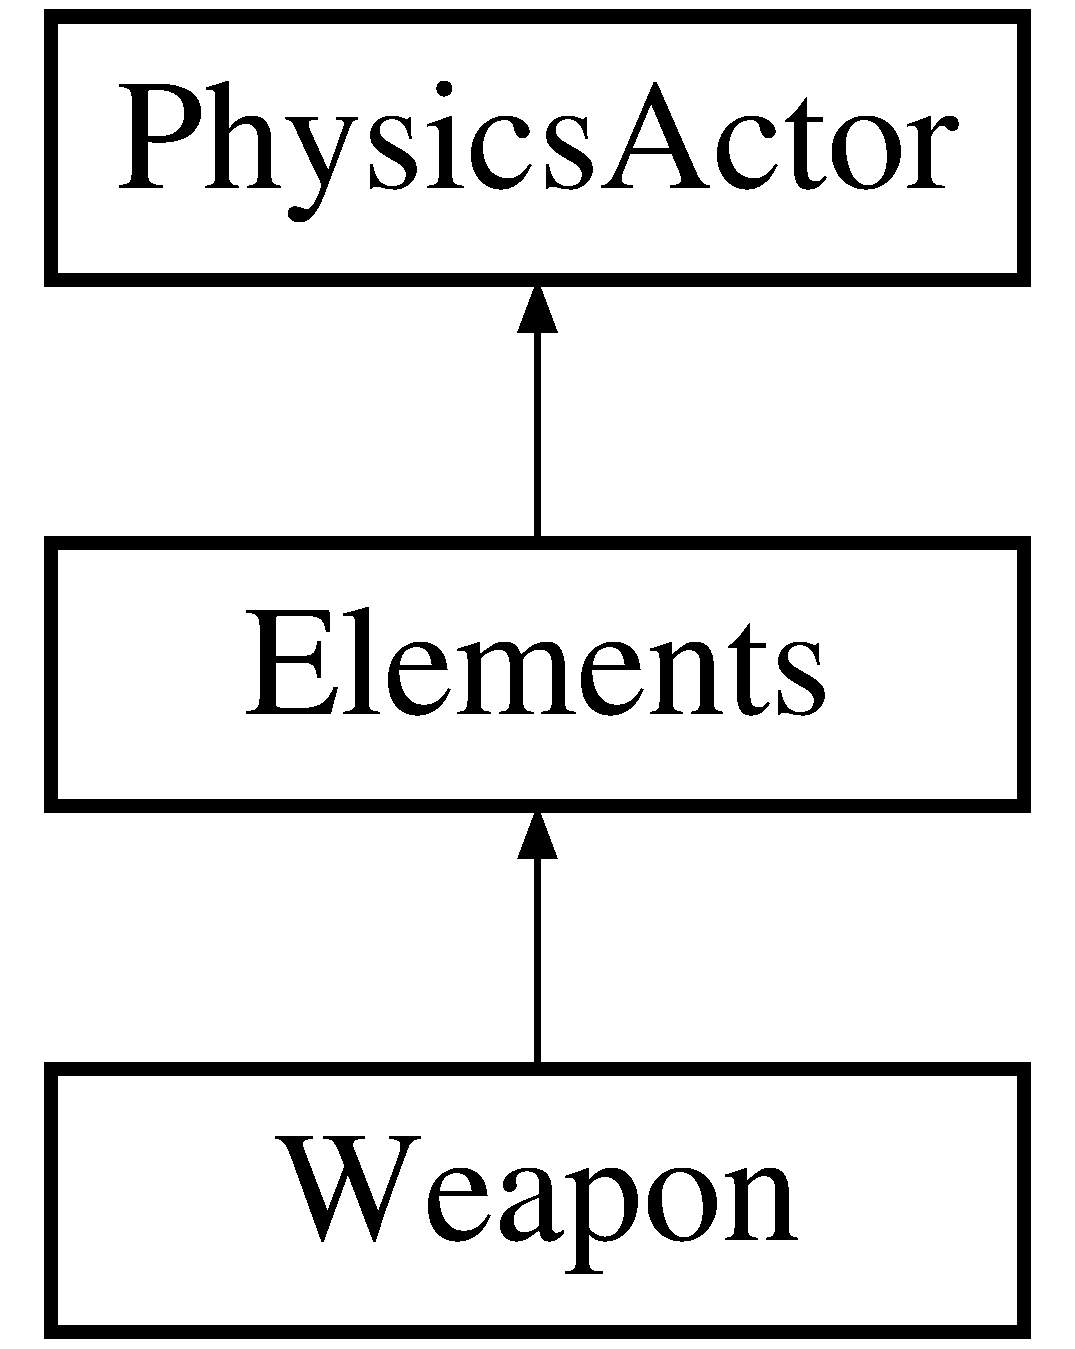
\includegraphics[height=3.000000cm]{class_weapon}
\end{center}
\end{figure}
\subsection*{Public Member Functions}
\begin{DoxyCompactItemize}
\item 
\hyperlink{class_weapon_a7267e890fa563b4f2df8746f443b461a}{Weapon} (std\+::string name)
\begin{DoxyCompactList}\small\item\em Constructor called by the weaponlist class to parse all weapons. \end{DoxyCompactList}\item 
\hyperlink{class_weapon_a559c41dbcc415a6ee70112f5231ef83b}{Weapon} (\hyperlink{class_weapon}{Weapon} $\ast$weapon)
\begin{DoxyCompactList}\small\item\em Constructor called by hero/equipment class, to copy a parsed version from weaponlist. \end{DoxyCompactList}\item 
\hyperlink{class_weapon_aa3eb21f28f64908763402004fa802b36}{Weapon} (\hyperlink{class_weapon}{Weapon} $\ast$weapon, \hyperlink{class_characters}{Characters} $\ast$c)
\begin{DoxyCompactList}\small\item\em Constructor called when attacking, creates the defined hitbox. \end{DoxyCompactList}\item 
\hypertarget{class_weapon_aa3364fb5092bbdb4c215e02dd1494f10}{\hyperlink{class_weapon_aa3364fb5092bbdb4c215e02dd1494f10}{$\sim$\+Weapon} (void)}\label{class_weapon_aa3364fb5092bbdb4c215e02dd1494f10}

\begin{DoxyCompactList}\small\item\em Basic destructor. \end{DoxyCompactList}\item 
void \hyperlink{class_weapon_a90b2b26acbbfc87a14786c8859e4a01d}{attack} (\hyperlink{class_characters}{Characters} $\ast$c)
\begin{DoxyCompactList}\small\item\em Function called when a character attacks, to create the hitbox depending if its ranged or melee. \end{DoxyCompactList}\item 
\hypertarget{class_weapon_a866884395ed4c0e7a972bb18e8d7d030}{void {\bfseries Begin\+Contact} (\hyperlink{class_elements}{Elements} $\ast$elem, b2\+Contact $\ast$contact)}\label{class_weapon_a866884395ed4c0e7a972bb18e8d7d030}

\item 
\hypertarget{class_weapon_a1860f840f8c75555de52450300139d9b}{void {\bfseries End\+Contact} (\hyperlink{class_elements}{Elements} $\ast$elem, b2\+Contact $\ast$contact)}\label{class_weapon_a1860f840f8c75555de52450300139d9b}

\item 
\hypertarget{class_weapon_ad93665811c3df9c05bb22b9a1a9c1a66}{void {\bfseries Receive\+Message} (Message $\ast$m)}\label{class_weapon_ad93665811c3df9c05bb22b9a1a9c1a66}

\item 
\hypertarget{class_weapon_aa49263888dca8ee505a95294371adbf6}{std\+::string {\bfseries get\+Name} (void)}\label{class_weapon_aa49263888dca8ee505a95294371adbf6}

\item 
\hypertarget{class_weapon_abe73556e16426da65572d7981dcc800f}{std\+::string {\bfseries get\+Flavor} (void)}\label{class_weapon_abe73556e16426da65572d7981dcc800f}

\item 
\hypertarget{class_weapon_a693e8f30f48b5df1983c22fdf796f25b}{std\+::string {\bfseries get\+Attack} (void)}\label{class_weapon_a693e8f30f48b5df1983c22fdf796f25b}

\item 
\hypertarget{class_weapon_ace3e431278e9ac23f33d222c67c38497}{std\+::string {\bfseries get\+Sprite} (void)}\label{class_weapon_ace3e431278e9ac23f33d222c67c38497}

\item 
\hypertarget{class_weapon_aea6024533cc9ca0ce72139ebf5da33f9}{float {\bfseries get\+Active} (void)}\label{class_weapon_aea6024533cc9ca0ce72139ebf5da33f9}

\item 
\hypertarget{class_weapon_a47baa57bfa8b9bfeda891d3180caa399}{int {\bfseries get\+Size} (void)}\label{class_weapon_a47baa57bfa8b9bfeda891d3180caa399}

\item 
\hypertarget{class_weapon_a64da6983673bfcac2d7de62ab92640f1}{int {\bfseries get\+Loot\+Level} (void)}\label{class_weapon_a64da6983673bfcac2d7de62ab92640f1}

\item 
\hypertarget{class_weapon_a35f92fc79c009c1d1d7d41b4fa17bb11}{int {\bfseries get\+Damage} (void)}\label{class_weapon_a35f92fc79c009c1d1d7d41b4fa17bb11}

\item 
\hypertarget{class_weapon_a60a49fa0a0a76a58698d9b4000815a8b}{int {\bfseries get\+Pushback} (void)}\label{class_weapon_a60a49fa0a0a76a58698d9b4000815a8b}

\item 
\hypertarget{class_weapon_a18a362244c6a169db89536505eaa2f15}{float {\bfseries get\+Recovery} (void)}\label{class_weapon_a18a362244c6a169db89536505eaa2f15}

\item 
\hypertarget{class_weapon_aded3e214d38d181504d49719cfc08fa5}{int {\bfseries attack\+Ready} (void)}\label{class_weapon_aded3e214d38d181504d49719cfc08fa5}

\item 
\hypertarget{class_weapon_a24f4509a23008f783c566ffa68548fb4}{void {\bfseries is\+Attacking} (int i)}\label{class_weapon_a24f4509a23008f783c566ffa68548fb4}

\end{DoxyCompactItemize}
\subsection*{Protected Member Functions}
\begin{DoxyCompactItemize}
\item 
Json\+::\+Value \hyperlink{class_weapon_ade3d2d4e411807411131b43238e47731}{\+\_\+get\+Attr} (std\+::string category, std\+::string key)
\begin{DoxyCompactList}\small\item\em Function called to get an attr value from the parsed json. \end{DoxyCompactList}\end{DoxyCompactItemize}
\subsection*{Additional Inherited Members}


\subsection{Constructor \& Destructor Documentation}
\hypertarget{class_weapon_a7267e890fa563b4f2df8746f443b461a}{\index{Weapon@{Weapon}!Weapon@{Weapon}}
\index{Weapon@{Weapon}!Weapon@{Weapon}}
\subsubsection[{Weapon}]{\setlength{\rightskip}{0pt plus 5cm}Weapon\+::\+Weapon (
\begin{DoxyParamCaption}
\item[{std\+::string}]{name}
\end{DoxyParamCaption}
)}}\label{class_weapon_a7267e890fa563b4f2df8746f443b461a}


Constructor called by the weaponlist class to parse all weapons. 

Licensed to the Apache Software Foundation (A\+S\+F) under one or more contributor license agreements. See the N\+O\+T\+I\+C\+E file distributed with this work for additional information regarding copyright ownership. The A\+S\+F licenses this file to you under the Apache License, Version 2.\+0 (the \char`\"{}\+License\char`\"{}); you may not use this file except in compliance with the License. You may obtain a copy of the License at

\href{http://www.apache.org/licenses/LICENSE-2.0}{\tt http\+://www.\+apache.\+org/licenses/\+L\+I\+C\+E\+N\+S\+E-\/2.\+0}

Unless required by applicable law or agreed to in writing, software distributed under the License is distributed on an \char`\"{}\+A\+S I\+S\char`\"{} B\+A\+S\+I\+S, W\+I\+T\+H\+O\+U\+T W\+A\+R\+R\+A\+N\+T\+I\+E\+S O\+R C\+O\+N\+D\+I\+T\+I\+O\+N\+S O\+F A\+N\+Y K\+I\+N\+D, either express or implied. See the License for the specific language governing permissions and limitations under the License. File\+: Weapon.\+cpp Creation\+: 2015-\/02-\/18 14\+:00 Vincent Rey \href{mailto:vrey@student.42.fr}{\tt vrey@student.\+42.\+fr} Default constructor, using the element that called the attack 
\begin{DoxyParams}{Parameters}
{\em name} & (std\+::string) \\
\hline
\end{DoxyParams}
\hypertarget{class_weapon_a559c41dbcc415a6ee70112f5231ef83b}{\index{Weapon@{Weapon}!Weapon@{Weapon}}
\index{Weapon@{Weapon}!Weapon@{Weapon}}
\subsubsection[{Weapon}]{\setlength{\rightskip}{0pt plus 5cm}Weapon\+::\+Weapon (
\begin{DoxyParamCaption}
\item[{{\bf Weapon} $\ast$}]{weapon}
\end{DoxyParamCaption}
)}}\label{class_weapon_a559c41dbcc415a6ee70112f5231ef83b}


Constructor called by hero/equipment class, to copy a parsed version from weaponlist. 

Copy constructor 
\begin{DoxyParams}{Parameters}
{\em weapon} & (Weapon$\ast$) \\
\hline
\end{DoxyParams}
\hypertarget{class_weapon_aa3eb21f28f64908763402004fa802b36}{\index{Weapon@{Weapon}!Weapon@{Weapon}}
\index{Weapon@{Weapon}!Weapon@{Weapon}}
\subsubsection[{Weapon}]{\setlength{\rightskip}{0pt plus 5cm}Weapon\+::\+Weapon (
\begin{DoxyParamCaption}
\item[{{\bf Weapon} $\ast$}]{w, }
\item[{{\bf Characters} $\ast$}]{c}
\end{DoxyParamCaption}
)}}\label{class_weapon_aa3eb21f28f64908763402004fa802b36}


Constructor called when attacking, creates the defined hitbox. 

Constructor for creating the weapon area-\/of-\/effect 
\begin{DoxyParams}{Parameters}
{\em w} & Weapon$\ast$ \\
\hline
{\em c} & (Characters$\ast$) \\
\hline
\end{DoxyParams}


\subsection{Member Function Documentation}
\hypertarget{class_weapon_ade3d2d4e411807411131b43238e47731}{\index{Weapon@{Weapon}!\+\_\+get\+Attr@{\+\_\+get\+Attr}}
\index{\+\_\+get\+Attr@{\+\_\+get\+Attr}!Weapon@{Weapon}}
\subsubsection[{\+\_\+get\+Attr}]{\setlength{\rightskip}{0pt plus 5cm}Json\+::\+Value Weapon\+::\+\_\+get\+Attr (
\begin{DoxyParamCaption}
\item[{std\+::string}]{category, }
\item[{std\+::string}]{key}
\end{DoxyParamCaption}
)\hspace{0.3cm}{\ttfamily [protected]}}}\label{class_weapon_ade3d2d4e411807411131b43238e47731}


Function called to get an attr value from the parsed json. 

Get a Json\+::\+Value of a key in the config file 
\begin{DoxyParams}{Parameters}
{\em } & category (std\+::string) \\
\hline
{\em } & key (std\+::string) \\
\hline
\end{DoxyParams}
\begin{DoxyNote}{Note}
\+: See the docs for the utilisation of Json\+::\+Value 
\end{DoxyNote}
\hypertarget{class_weapon_a90b2b26acbbfc87a14786c8859e4a01d}{\index{Weapon@{Weapon}!attack@{attack}}
\index{attack@{attack}!Weapon@{Weapon}}
\subsubsection[{attack}]{\setlength{\rightskip}{0pt plus 5cm}void Weapon\+::attack (
\begin{DoxyParamCaption}
\item[{{\bf Characters} $\ast$}]{c}
\end{DoxyParamCaption}
)}}\label{class_weapon_a90b2b26acbbfc87a14786c8859e4a01d}


Function called when a character attacks, to create the hitbox depending if its ranged or melee. 

Called by the Character to attack with the currently equipped weapon 
\begin{DoxyParams}{Parameters}
{\em } & x (Int) \\
\hline
{\em } & y (Int) \\
\hline
{\em } & orientation\+X (int) \\
\hline
{\em } & orientation\+Y (int) \\
\hline
{\em } & linear\+Velocity (b2\+Vec2) \\
\hline
\end{DoxyParams}


The documentation for this class was generated from the following files\+:\begin{DoxyCompactItemize}
\item 
inc/Weapon.\+hpp\item 
src/Weapon.\+cpp\end{DoxyCompactItemize}

\hypertarget{class_weapon_list}{\section{Weapon\+List Class Reference}
\label{class_weapon_list}\index{Weapon\+List@{Weapon\+List}}
}


{\ttfamily \#include $<$Weapon\+List.\+hpp$>$}

Inheritance diagram for Weapon\+List\+:\begin{figure}[H]
\begin{center}
\leavevmode
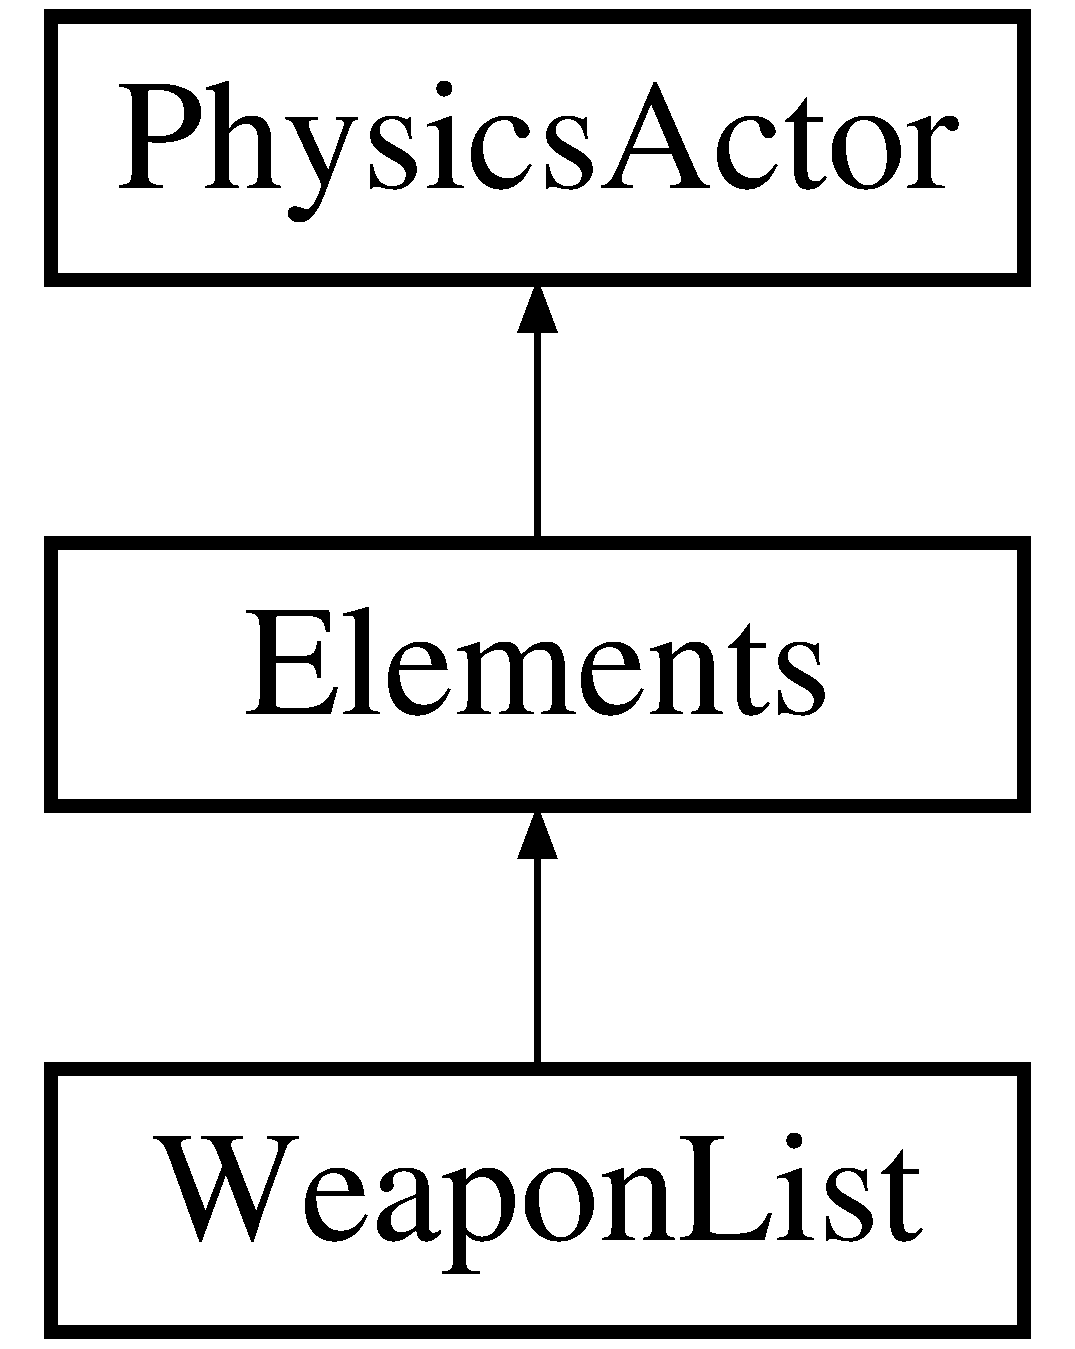
\includegraphics[height=3.000000cm]{class_weapon_list}
\end{center}
\end{figure}
\subsection*{Public Member Functions}
\begin{DoxyCompactItemize}
\item 
\hyperlink{class_weapon_list_ac3a994cd2844ac00fcf09011f4209f48}{Weapon\+List} (void)
\begin{DoxyCompactList}\small\item\em Constructor called at the beginning of the game to load every weapon available. \end{DoxyCompactList}\item 
\hyperlink{class_weapon_list_a44f72440d8a4586b19e4b60d308b2e51}{$\sim$\+Weapon\+List} (void)
\begin{DoxyCompactList}\small\item\em Destructor. \end{DoxyCompactList}\item 
\hypertarget{class_weapon_list_ad39bd93b72f73eb7e69388dd5d4bfac2}{void {\bfseries stat\+Weapon} (std\+::string)}\label{class_weapon_list_ad39bd93b72f73eb7e69388dd5d4bfac2}

\item 
\hyperlink{class_weapon}{Weapon} $\ast$ \hyperlink{class_weapon_list_a97b9173cefa20573ed27d52d58d1292e}{get\+Weapon} (std\+::string)
\begin{DoxyCompactList}\small\item\em Returns a weapon in order to use it afterwards. \end{DoxyCompactList}\item 
\hyperlink{class_weapon}{Weapon} $\ast$ \hyperlink{class_weapon_list_aee801adca4fe1154993eedc6c71b3dca}{get\+Weapon\+Random} (void)
\begin{DoxyCompactList}\small\item\em Returns one of the existing weapons. \end{DoxyCompactList}\item 
\hyperlink{class_weapon}{Weapon} $\ast$ \hyperlink{class_weapon_list_a80b1e46c7e1fa0e6be725fe8d13ed93d}{get\+Weapon\+Random} (int level)
\begin{DoxyCompactList}\small\item\em Returns one of the existing weapons of the required level. \end{DoxyCompactList}\end{DoxyCompactItemize}
\subsection*{Additional Inherited Members}


\subsection{Detailed Description}
Licensed to the Apache Software Foundation (A\+S\+F) under one or more contributor license agreements. See the N\+O\+T\+I\+C\+E file distributed with this work for additional information regarding copyright ownership. The A\+S\+F licenses this file to you under the Apache License, Version 2.\+0 (the \char`\"{}\+License\char`\"{}); you may not use this file except in compliance with the License. You may obtain a copy of the License at

\href{http://www.apache.org/licenses/LICENSE-2.0}{\tt http\+://www.\+apache.\+org/licenses/\+L\+I\+C\+E\+N\+S\+E-\/2.\+0}

Unless required by applicable law or agreed to in writing, software distributed under the License is distributed on an \char`\"{}\+A\+S I\+S\char`\"{} B\+A\+S\+I\+S, W\+I\+T\+H\+O\+U\+T W\+A\+R\+R\+A\+N\+T\+I\+E\+S O\+R C\+O\+N\+D\+I\+T\+I\+O\+N\+S O\+F A\+N\+Y K\+I\+N\+D, either express or implied. See the License for the specific language governing permissions and limitations under the License. File\+: \hyperlink{_weapon_list_8hpp_source}{Weapon\+List.\+hpp} Creation\+: 2015-\/02-\/18 14\+:00 Vincent Rey \href{mailto:vrey@student.42.fr}{\tt vrey@student.\+42.\+fr} 

\subsection{Constructor \& Destructor Documentation}
\hypertarget{class_weapon_list_ac3a994cd2844ac00fcf09011f4209f48}{\index{Weapon\+List@{Weapon\+List}!Weapon\+List@{Weapon\+List}}
\index{Weapon\+List@{Weapon\+List}!Weapon\+List@{Weapon\+List}}
\subsubsection[{Weapon\+List}]{\setlength{\rightskip}{0pt plus 5cm}Weapon\+List\+::\+Weapon\+List (
\begin{DoxyParamCaption}
\item[{void}]{}
\end{DoxyParamCaption}
)}}\label{class_weapon_list_ac3a994cd2844ac00fcf09011f4209f48}


Constructor called at the beginning of the game to load every weapon available. 

Licensed to the Apache Software Foundation (A\+S\+F) under one or more contributor license agreements. See the N\+O\+T\+I\+C\+E file distributed with this work for additional information regarding copyright ownership. The A\+S\+F licenses this file to you under the Apache License, Version 2.\+0 (the \char`\"{}\+License\char`\"{}); you may not use this file except in compliance with the License. You may obtain a copy of the License at

\href{http://www.apache.org/licenses/LICENSE-2.0}{\tt http\+://www.\+apache.\+org/licenses/\+L\+I\+C\+E\+N\+S\+E-\/2.\+0}

Unless required by applicable law or agreed to in writing, software distributed under the License is distributed on an \char`\"{}\+A\+S I\+S\char`\"{} B\+A\+S\+I\+S, W\+I\+T\+H\+O\+U\+T W\+A\+R\+R\+A\+N\+T\+I\+E\+S O\+R C\+O\+N\+D\+I\+T\+I\+O\+N\+S O\+F A\+N\+Y K\+I\+N\+D, either express or implied. See the License for the specific language governing permissions and limitations under the License. File\+: Weapon\+List.\+cpp Creation\+: 2015-\/02-\/18 14\+:00 Vincent Rey \href{mailto:vrey@student.42.fr}{\tt vrey@student.\+42.\+fr} Called once and stocked in a static for the whole game \hypertarget{class_weapon_list_a44f72440d8a4586b19e4b60d308b2e51}{\index{Weapon\+List@{Weapon\+List}!````~Weapon\+List@{$\sim$\+Weapon\+List}}
\index{````~Weapon\+List@{$\sim$\+Weapon\+List}!Weapon\+List@{Weapon\+List}}
\subsubsection[{$\sim$\+Weapon\+List}]{\setlength{\rightskip}{0pt plus 5cm}Weapon\+List\+::$\sim$\+Weapon\+List (
\begin{DoxyParamCaption}
\item[{void}]{}
\end{DoxyParamCaption}
)}}\label{class_weapon_list_a44f72440d8a4586b19e4b60d308b2e51}


Destructor. 

Basic destructor 

\subsection{Member Function Documentation}
\hypertarget{class_weapon_list_a97b9173cefa20573ed27d52d58d1292e}{\index{Weapon\+List@{Weapon\+List}!get\+Weapon@{get\+Weapon}}
\index{get\+Weapon@{get\+Weapon}!Weapon\+List@{Weapon\+List}}
\subsubsection[{get\+Weapon}]{\setlength{\rightskip}{0pt plus 5cm}{\bf Weapon} $\ast$ Weapon\+List\+::get\+Weapon (
\begin{DoxyParamCaption}
\item[{std\+::string}]{name}
\end{DoxyParamCaption}
)}}\label{class_weapon_list_a97b9173cefa20573ed27d52d58d1292e}


Returns a weapon in order to use it afterwards. 

Get a weapon obj by name 
\begin{DoxyParams}{Parameters}
{\em name} & (std\+::string) \\
\hline
\end{DoxyParams}
\begin{DoxyReturn}{Returns}
$\ast$it 
\end{DoxyReturn}
\hypertarget{class_weapon_list_aee801adca4fe1154993eedc6c71b3dca}{\index{Weapon\+List@{Weapon\+List}!get\+Weapon\+Random@{get\+Weapon\+Random}}
\index{get\+Weapon\+Random@{get\+Weapon\+Random}!Weapon\+List@{Weapon\+List}}
\subsubsection[{get\+Weapon\+Random}]{\setlength{\rightskip}{0pt plus 5cm}{\bf Weapon} $\ast$ Weapon\+List\+::get\+Weapon\+Random (
\begin{DoxyParamCaption}
\item[{void}]{}
\end{DoxyParamCaption}
)}}\label{class_weapon_list_aee801adca4fe1154993eedc6c71b3dca}


Returns one of the existing weapons. 

Returns a weapon, no matter its level \hypertarget{class_weapon_list_a80b1e46c7e1fa0e6be725fe8d13ed93d}{\index{Weapon\+List@{Weapon\+List}!get\+Weapon\+Random@{get\+Weapon\+Random}}
\index{get\+Weapon\+Random@{get\+Weapon\+Random}!Weapon\+List@{Weapon\+List}}
\subsubsection[{get\+Weapon\+Random}]{\setlength{\rightskip}{0pt plus 5cm}{\bf Weapon} $\ast$ Weapon\+List\+::get\+Weapon\+Random (
\begin{DoxyParamCaption}
\item[{int}]{level}
\end{DoxyParamCaption}
)}}\label{class_weapon_list_a80b1e46c7e1fa0e6be725fe8d13ed93d}


Returns one of the existing weapons of the required level. 

Returns a random weapon, with the corresponding item level 

The documentation for this class was generated from the following files\+:\begin{DoxyCompactItemize}
\item 
inc/Weapon\+List.\+hpp\item 
src/Weapon\+List.\+cpp\end{DoxyCompactItemize}

%--- End generated contents ---

% Index
\newpage
\phantomsection
\addcontentsline{toc}{part}{Index}
\printindex

\end{document}
